\documentclass[oldfontcommands,a4paper]{memoir}

\usepackage[T1]{fontenc}
\usepackage[utf8]{inputenc}
\usepackage[a4paper]{geometry}
\geometry{verbose,tmargin=2.5cm,bmargin=2.5cm,lmargin=2.5cm,rmargin=2.5cm}
\pagestyle{Ruled}
\usepackage{array}
\usepackage{verbatim}
\usepackage{prettyref}
\usepackage{booktabs}
\usepackage{textcomp}
\usepackage{url}
\usepackage{amsmath}
\usepackage{chemarr}%flechas para reacciones químicas (SFER.tex)
\usepackage{graphicx}
\usepackage{amssymb}
\usepackage{nomencl}
\usepackage[usenames,dvipsnames]{xcolor}
\usepackage{enumitem}
% the following is useful when we have the old nomencl.sty package
% \providecommand{\printnomenclature}{\printglossary}
% \providecommand{\makenomenclature}{\makeglossary}
\makenomenclature

\usepackage{subfig}
%Configuración de los caption
\PassOptionsToPackage{caption=false}{subfig}%Evita que el paquete subfig lo descabale todo
\captiontitlefont{\itshape}
\captionnamefont{\scshape}
\captionstyle{\centering}
\hangcaption
\usepackage{cancel}
\usepackage{steinmetz}
\usepackage{diffcoeff}
\usepackage{mathtools}

\newtheorem{exerciseT}{Ejemplo}[chapter]

\usepackage[spanish]{babel}
\addto\shorthandsspanish{\spanishdeactivate{~<>}}


\usepackage{siunitx}
\DeclareSIUnit\kWh{kWh}
\DeclareSIUnit{\watthour}{Wh}
\DeclareSIUnit\Wh{Wh}
\DeclareSIUnit{\voltampere}{VA}
\DeclareSIUnit{\var}{var}

\sisetup{per-mode=symbol-or-fraction}
%\usepackage{lscape}
\usepackage{mathpazo}%Letra palatino con fuentes para matemáticas
\usepackage{flafter}%obliga a que los flotantes aparezcan después de su referencia
\usepackage{memhfixc}

\usepackage{xparse} % For "overbrace/underbrace but with an arrow instead", from https://tex.stackexchange.com/questions/8720/overbrace-underbrace-but-with-an-arrow-instead

% Para poner flechas sobre los signos de igual, de aquí: https://tex.stackexchange.com/questions/8720/overbrace-underbrace-but-with-an-arrow-instead
\NewDocumentCommand{\overarrow}{O{=} O{\uparrow} m}{%
  \overset{\makebox[0pt]{\begin{tabular}{@{}c@{}}#3\\[0pt]\ensuremath{#2}\end{tabular}}}{#1}
}
\NewDocumentCommand{\underarrow}{O{=} O{\downarrow} m}{%
  \underset{\makebox[0pt]{\begin{tabular}{@{}c@{}}\ensuremath{#2}\\[0pt]#3\end{tabular}}}{#1}
}

\usepackage{rotating,stackengine,scalerel}
\newcommand\wye{\scalerel*{\stackengine{-1pt}{%
  \rotatebox[origin=c]{30}{\rule{10pt}{.9pt}}\kern-1pt%
  \rotatebox[origin=c]{-30}{\rule{10pt}{1.3pt}}}{%
  \rule{.9pt}{10pt}}{O}{c}{F}{F}{S}}{\Delta}} % https://tex.stackexchange.com/questions/481532/star-wye-electrical-connection-math-symbol
  
\raggedbottom
\sloppybottom
\clubpenalty=10000
\widowpenalty=10000

%\raggedbottomsection
\feetbelowfloat


% \usepackage[citestyle=alphabetic, bibstyle=alphabetic, maxbibnames=5,minbibnames=3,
% backend=bibtex, doi=true, url=true]{biblatex}

% \DefineBibliographyStrings{spanish}{%
%   andothers        = {et\addabbrvspace al\adddot},
%   andmore          = {et\addabbrvspace al\adddot},
%   in               = {},
% }

% \let\cite\parencite

% \renewcommand{\bibsection}{%
% 	\chapter*{\bibname}
% 	\bibmark
% 	\phantomsection
% 	\addcontentsline{toc}{chapter}{\bibname}
% 	\prebibhook}
% % \renewcommand{\bbltechreport}{Informe T\'ecnico}


\usepackage{hyperref}


\hypersetup{
    bookmarks=true,         % show bookmarks bar?
    unicode=true,          % non-Latin characters in Acrobat’s bookmarks
    bookmarksnumbered=false,
    bookmarksopen=false,
    breaklinks=true,
    backref=true,
    pdftoolbar=true,        % show Acrobat’s toolbar?
    pdfmenubar=true,        % show Acrobat’s menu?
    pdffitwindow=false,     % window fit to page when opened
    pdfstartview={FitH},    % fits the width of the page to the window
    pdftitle={Teoria de Circuitos},    % title
    pdfsubject={ETSIDI},   % subject of the document
    pdfcreator={Overleaf},   % creator of the document
    pdfproducer={LaTeX}, % producer of the document
    pdfnewwindow=true,      % links in new window
    pdfborder={0 0 0},
    colorlinks=true,       % false: boxed links; true: colored links
    linkcolor=Brown,          % color of internal links
    citecolor=BrickRed,        % color of links to bibliography
    filecolor=black,      % color of file links
    urlcolor=Blue           % color of external links 
}

\addto\captionsspanish{%
\def\tablename{Tabla}%
\def\listtablename{\'Indice de tablas}}


%\spanishdecimal{.} %Para que no lo sustituya automáticamente por comas
%\def\nompreamble{\addcontentsline{toc}{chapter}{\nomname}\markboth{\nomname}{\nomname}}

%Configuración de MEMOIR
%%Pone la fecha en SMALL CAPS y hacia la derecha
%%pagina 60 de memman.pdf
\pretitle{
  \vfill
  \centering \bfseries \scshape \HUGE \color{BrickRed}
}

\posttitle{\par}

\preauthor{
  \vfill
  \centering
  \large \scshape
}
\postauthor{\par }

\predate{\vfill \begin{flushright}\large\scshape}
\postdate{\par\end{flushright}\vfill}


\setsecnumdepth{subsection}


% \definecolor{ared}{rgb}{.647,.129,.149}
% \renewcommand{\colorchapnum}{\color{ared}}
% \renewcommand{\colorchaptitle}{\color{ared}}
% \chapterstyle{pedersen}
\chapterstyle{ger}

\setlength{\afterchapskip}{35pt}
\maxtocdepth{subsection}

%\setcounter{topnumber}{3}
%\setcounter{bottomnumber}{2}
%\setcounter{totalnumber}{4}
\renewcommand{\topfraction}{0.85}
\renewcommand{\bottomfraction}{0.5}
\renewcommand{\textfraction}{0.15}
\renewcommand{\floatpagefraction}{0.7}


\usepackage{float}

\RequirePackage[framemethod=default]{mdframed} % Required for creating the theorem, definition, exercise and corollary boxes

% Exercise box	  
\newmdenv[skipabove=7pt,
skipbelow=7pt,
rightline=false,
leftline=false,
topline=false,
bottomline=false,
backgroundcolor=MidnightBlue!5,
linecolor=MidnightBlue,
innerleftmargin=5pt,
innerrightmargin=5pt,
innertopmargin=5pt,
innerbottommargin=5pt,
leftmargin=0cm,
rightmargin=0cm,
linewidth=4pt]{eBox}

\newenvironment{example}{\begin{eBox}\begin{exerciseT}}{\hfill{\color{MidnightBlue}\tiny\ensuremath{\blacksquare}}\end{exerciseT}\end{eBox}}	


\renewcommand{\textfloatsep}{10pt}%Espacio entre el flotante y el texto

\usepackage{tikz}
\newenvironment{remark}{\par\vspace{10pt}\small % Vertical white space above the remark and smaller font size
\begin{list}{}{
\leftmargin=35pt % Indentation on the left
\rightmargin=25pt}\item\ignorespaces % Indentation on the right
\makebox[-2.5pt]{\begin{tikzpicture}[overlay]
\node[draw=MidnightBlue!60,line width=1pt,circle,fill=MidnightBlue!25,font=\sffamily\bfseries,inner sep=2pt,outer sep=0pt] at (-15pt,0pt){\textcolor{MidnightBlue}{N}};\end{tikzpicture}} % Orange R in a circle
\advance\baselineskip -1pt}{\end{list}\vskip5pt} % Tighter line spacing and white space after remark 

\setcounter{tocdepth}{0}

\begin{document}


%\pagestyle{empty}
\begin{titlingpage}

\title{Problemas Resueltos\\ de\\ Teoría de Circuitos}

\author{
  Luis Badesa Bernardo\\
  Carmelo Carrero López\\
  Ana Fernández Guillamón\\
  Ricardo Granizo Arrabé\\
  Oscar Perpiñán Lamigueiro}
 
\date{
  Universidad Politécnica de Madrid}

\maketitle


\end{titlingpage}

\frontmatter


\chapterprecis{\vfill{}
}
\rule[.5ex]{\linewidth}{1pt} 

Julio de 2023

© 2023 Luis Badesa Bernardo, Ana Fernández Guillamón, Oscar Perpiñán Lamigueiro

Este documento está accesible en \url{https://github.com/ETSIDI-IE/tc}

\begin{center}

\includegraphics[scale=0.5]{../figs/cc-logo}
\par\end{center}

Esta obra está bajo una licencia \textbf{Reconocimiento-No comercial-Compartir
bajo la misma licencia} 4.0 España de Creative Commons. Para ver una
copia de esta licencia, visite:\\
 \url{https://creativecommons.org/licenses/by-nc-sa/4.0/deed.es_ES}

Usted es libre de copiar, distribuir y comunicar públicamente la obra,
y hacer obras derivadas bajo las condiciones siguientes:
\begin{itemize}
\item 
\includegraphics[scale=0.35]{../figs/by} \textbf{Reconocimiento}.
Debe reconocer adecuadamente la autoría, proporcionar un enlace a la licencia e indicar si se han realizado cambios. Puede hacerlo de cualquier manera razonable, pero no de una manera que sugiera que tiene el apoyo del licenciador o lo recibe por el uso que hace.
\item 
\includegraphics[scale=0.35]{../figs/nc-eu} \textbf{No comercial}.
No puede utilizar el material para una finalidad comercial.
\item 
\includegraphics[scale=0.35]{../figs/sa} \textbf{Compartir bajo la
misma licencia}.  Si remezcla, transforma o crea a partir del material, deberá difundir sus contribuciones bajo la misma licencia que el original.
\end{itemize}
Al reutilizar o distribuir la obra, tiene que dejar bien claro los
términos de la licencia de esta obra. Alguna de estas condiciones
puede no aplicarse si se obtiene el permiso del titular de los derechos
de autor. Nada en esta licencia menoscaba o restringe los derechos
morales del autor.

%%% Local Variables:
%%% mode: LaTex
%%% TeX-master: "TC.tex"
%%% End: 

\tableofcontents*
% \clearpage
% \listoffigures*
% \clearpage
% \listoftables*

\cleardoublepage{}

\mainmatter

\chapter{Corriente continua}

\section{Enunciado}
Calcular las corrientes de malla mostradas en el circuito de la
figura.

\vspace{2mm}
Datos: $\; R_1 = \qty{2}{\ohm}$;\; $R_2 = \qty{5}{\ohm}$;\; $R_3 = \qty{10}{\ohm}$;\; $R_4 = \qty{4}{\ohm}$;\; $R_5 = \qty{2}{\ohm}$;\; $E_1 = \qty{25}{\volt}$;\; $E_2 = \qty{50}{\volt}$

\begin{center}
  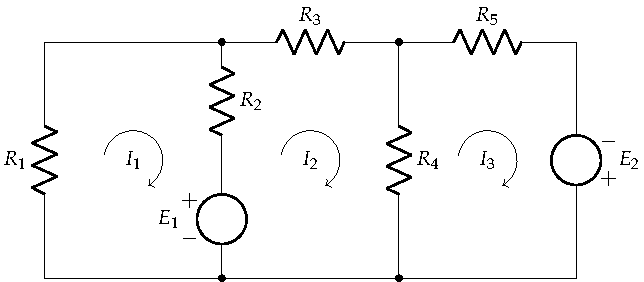
\includegraphics{figuras/BT1_02.pdf}
\end{center}

  

  \subsection*{Solución}
  Se plantea el sistema de ecuaciones en forma matricial, siendo de la forma $[R]\cdot[I]=[U]$. Cada $R_{i,i}$ de la matriz $[R]$ se corresponde con la suma de resistencias incluidas en la malla $i$; cada $\pm R_{ij}$ se corresponde con la suma de las resistencias incluidas en las ramas compartidas por las mallas $i$ y $j$, con signo positivo ($+$) si las corrientes van en el mismo sentido, y negativo ($-$) en caso contrario; y cada $\sum \epsilon_i$ es la suma algebraica de las fuerzas electromotrices de los generadores de la malla $i$, considerando un signo positivo ($+$) si contribuyen al giro de la corriente, y negativo ($-$) en caso contrario (es decir, si la corriente sale por el polo $+$ de la fuente, se considera positivo; si sale por el polo $-$, se considera negativo). Así:
  \begin{equation*}
    \begin{bmatrix}
      R_1+R_2 & -R_2 & 0 \\
      -R_2 & R_2+R_3+R_4 & -R_4 \\
      0 & -R_4 & R_4+R_5
    \end{bmatrix} \cdot
    \begin{bmatrix}
      I_1\\
      I_2\\
      I_3
    \end{bmatrix} = %
    \begin{bmatrix}
      -E_1 \\
      E_1\\
      E_2
    \end{bmatrix}
  \end{equation*}
  Reemplazando con los valores correspondientes, el sistema a resolver es:
  \begin{equation*}
    \begin{bmatrix}
      7 & -5 & 0 \\
      -5 & 19 & -4 \\
      0 & -4 & 6
    \end{bmatrix} \cdot
    \begin{bmatrix}
      I_1\\
      I_2\\
      I_3
    \end{bmatrix} = %
    \begin{bmatrix}
      -25 \\
      25\\
      50
    \end{bmatrix}
  \end{equation*}
  cuya solución es:
  \begin{align*}
    I_1&=\qty{-1.31}{\ampere}\\
    I_2&=\qty{3.17}{\ampere}\\
    I_3&=\qty{10.45}{\ampere}
  \end{align*}


%%%%%%%%%%%%%%%%%%%%%%%%%%%%%%%%%%%%%%%%%%%%%%%%%%%%%%%%%%%%%%%%%%%%%%%%%

  \section{Enunciado}
  Calcular el valor de $E$ que hace que $I_0=\qty{7.5}{\milli\ampere}$
  en el circuito de la figura.

\vspace{2mm}
Datos: $\; R_1 = \qty{8}{\ohm}$;\; $R_2 = \qty{7}{\ohm}$;\; $R_3 = \qty{4}{\ohm}$,\; $R_4 = \qty{6}{\ohm}$;\; $R_5 = \qty{6}{\ohm}$;\; $R_6 = \qty{12}{\ohm}$

  \begin{center}
    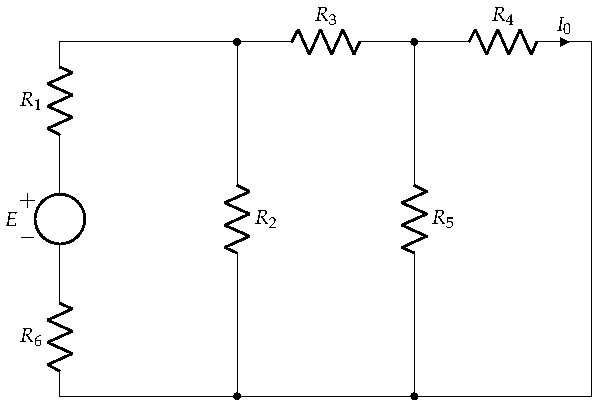
\includegraphics{figuras/BT1_03.pdf}
  \end{center}
   

\subsection*{Solución}
Siguiendo las mismas consideraciones del ejercicio anterior, se plantea el sistema de ecuaciones en forma matricial, suponiendo que
las tres corrientes de malla van en sentido horario:
\begin{equation*}
  \begin{bmatrix}
    R_1+R_2+R_6 & -R_2 & 0 \\
    -R_2 & R_2+R_3+R_5 & -R_5 \\
    0 & -R_5 & R_4+R_5
  \end{bmatrix} \cdot
  \begin{bmatrix}
    I_a\\
    I_b\\
    I_c
  \end{bmatrix} = %
  \begin{bmatrix}
    E \\
    0\\
    0
  \end{bmatrix}
\end{equation*}
Reemplazando con los valores correspondientes, el sistema a resolver es:
\begin{equation*}
  \begin{bmatrix}
    27 & -7 & 0 \\
    -7 & 17 & -6 \\
    0 & -6 & 12
  \end{bmatrix} \cdot
  \begin{bmatrix}
    I_a\\
    I_b\\
    I_c
  \end{bmatrix} = %
  \begin{bmatrix}
    E \\
    0\\
    0
  \end{bmatrix}
\end{equation*}
donde además se sabe el valor de $I_c=I_0=\qty{7.5}{\milli\ampere}$. Por
tanto, de la tercera ecuación se puede obtener el valor de $I_b$:
\begin{equation*}
  -6\,I_b+12\,I_c=-6\,I_b+12\cdot 7.5 = 0 \quad \Rightarrow \quad 6\,I_b=90 \quad \Rightarrow \quad I_b=\dfrac{90}{6}=\qty{15}{\milli\ampere}
\end{equation*}
Con $I_b$ calculado, se utiliza la segunda ecuación para determinar
$I_a$:
\begin{equation*}
  -7\,I_a+17\,I_b-6\,I_c=-7\,I_a+17\cdot 15-6\cdot 7.5 = 0\quad \Rightarrow \quad 7\,I_a=210\quad \Rightarrow \quad I_a=\dfrac{210}{7}=\qty{30}{\milli\ampere}
\end{equation*}
Determinada $I_a$, se emplea la primera ecuación para obtener el valor
de $E$:
\begin{equation*}
  27\,I_a-7\,I_b=27\cdot 30 - 7 \cdot 15 = E = {\qty{705}{\milli\volt}}
\end{equation*}


%%%%%%%%%%%%%%%%%%%%%%%%%%%%%%%%%%%%%%%%%%%%%%%%%%%%%%%%%%%%%%%%%%%%%%%%%

\section{Enunciado}
Calcular la intensidad $I$ en el circuito de la figura.

\vspace{2mm}
  Datos: $\; R_1 = \qty{27}{\ohm}$;\; $R_2 = \qty{47}{\ohm}$;\; $R_3 = \qty{27}{\ohm}$;\; $E_1 = \qty{460}{\volt}$;\; $E_2 = \qty{200}{\volt}$
  
\begin{center}
  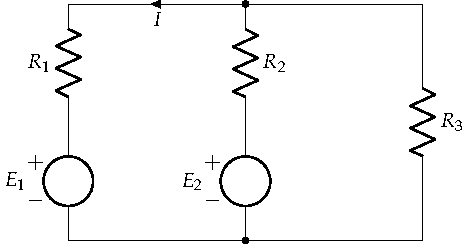
\includegraphics{figuras/BT1_04.pdf}
\end{center}


\subsection*{Solución}
Se suponen las mallas mostradas en la siguiente figura.

\begin{center}
  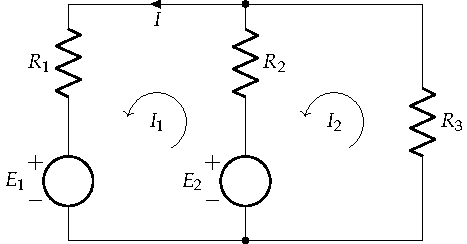
\includegraphics{figuras/BT1_04_mallas.pdf}
\end{center}

Se plantea el sistema de ecuaciones en forma matricial:
\begin{equation*}
  \begin{bmatrix}
    74 & -47  \\
    -47 & 74
  \end{bmatrix} \cdot
  \begin{bmatrix}
    I_1\\
    I_2
  \end{bmatrix} =
  \begin{bmatrix}
    -260 \\
    -200
  \end{bmatrix}
\end{equation*}
cuya solución es:
\begin{align*}
  I_1&=\qty{-8.77}{\ampere}\\
  I_2&=\qty{-8.27}{\ampere}
\end{align*}

%%%%%%%%%%%%%%%%%%%%%%%%%%%%%%%%%%%%%%%%%%%%%%%%%%%%%%%%%%%%%%%%%%
\section{Enunciado}
En el circuito de la figura obtener las intensidades de corriente
señaladas primero mediante un análisis por el método de las mallas y
posteriormente mediante un análisis por el método de los nudos.

\vspace{2mm}
Datos: $\; R_1 = \qty{2}{\ohm}$;\; $R_2 = \qty{1}{\ohm}$;\; $R_3 = \qty{4}{\ohm}$;\; $R_4 = \qty{5}{\ohm}$;\; $R_5 = \qty{3}{\ohm}$;\; $E_1 = \qty{10}{\volt}$;\; $E_2 = \qty{6}{\volt}$

\begin{center}
  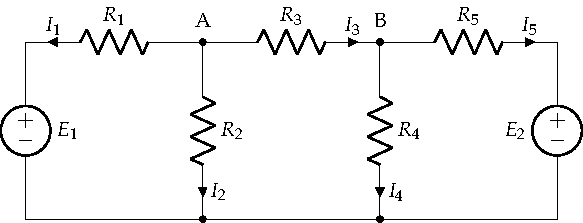
\includegraphics{figuras/BT1_08.pdf}
\end{center}
  

\subsection*{Solución}
Se aplica primero el método de las mallas, considerando las corrientes
de malla mostradas en la siguiente figura:
\begin{center}
  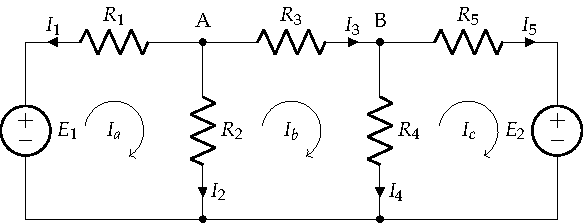
\includegraphics{figuras/BT1_08_mallas.pdf}
\end{center}

Se plantea el sistema de ecuaciones en forma matricial:
\begin{equation*}
  \begin{bmatrix}
    3 & -1 & 0 \\
    -1 & 10 & -5 \\
    0 & -5 & 8
  \end{bmatrix} \cdot
  \begin{bmatrix}
    I_a\\
    I_b\\
    I_c
  \end{bmatrix} = %
  \begin{bmatrix}
    10 \\
    0\\
    -6
  \end{bmatrix}
\end{equation*}
cuya solución es:
\begin{align*}
  I_a&=\qty{3.31}{\ampere}\\
  I_b&=\qty{-0.06}{\ampere}\\
  I_c&= \qty{-0.79}{\ampere}
\end{align*}
Se establecen las igualdades entre las diferentes corrientes de rama y
de malla, y se calculan sus valores:
\begin{align*}
  I_1&=-I_a=\qty{-3.31}{\ampere}\\
  I_2&=I_a-I_b=3.31-(-0.06)=\qty{3.37}{\ampere}\\
  I_3&=I_b=\qty{-0.06}{\ampere}\\
  I_4&=I_b-I_c=-0.06-(-0.79)=\qty{0.73}{\ampere}\\
  I_5&=I_c=\qty{-0.79}{\ampere}
\end{align*}
	
Para poder aplicar el método de los nudos, es necesario hacer, en
primer lugar, la transformación de las fuentes de tensión (y la
resistencia en serie) en fuentes de corriente (con una resistencia en
paralelo):
\begin{align*}
  I_{g,10V}&=\dfrac{\epsilon_{10V}}{R_{2\Omega}}=\dfrac{10}{2}=\qty{5}{\ampere}\\
  I_{g,6V}&=\dfrac{\epsilon_{6V}}{R_{3\Omega}}=\dfrac{6}{3}=\qty{2}{\ampere}
\end{align*}
quedando el circuito que se muestra a continuación.

\begin{center}
  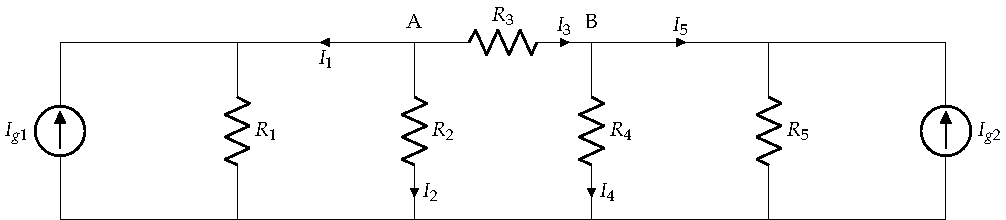
\includegraphics{figuras/BT1_08_nudos.pdf}
\end{center}

En este caso, se trabaja con las conductancias ($G=1/R$). Se
escribe el sistema de ecuaciones en modo matricial:
\begin{equation*}
  \begin{bmatrix}
    1.75 & - 0.25\\
    -0.25 & 0.783
  \end{bmatrix} \cdot%
  \begin{bmatrix}
    U_A\\
    U_B
  \end{bmatrix} = %
  \begin{bmatrix}
    5\\
    2
  \end{bmatrix}
\end{equation*}
cuya solución es:
\begin{align*}
  U_A&=\qty{3.38}{\volt}\\
  U_B&=\qty{3.63}{\volt}
\end{align*}
Con estos valores, se pueden determinar directamente las corrientes
$I_2$ e $I_4$, por simple aplicación de la ley de Ohm:
\begin{align*}
  I_2&=\dfrac{U_A}{R_{1\Omega}}=\dfrac{3.38}{1}=\qty{3.38}{\ampere}\\
  I_4&=\dfrac{U_B}{R_{5\Omega}}=\dfrac{3.63}{5}=\qty{0.73}{\ampere}
\end{align*}
Las corrientes que circulan por las resistencias en paralelo con las
fuentes de tensión se determinan de manera análoga:
\begin{align*}
  I_{2\Omega}&=\dfrac{U_A}{R_{2\Omega}}=\dfrac{3.38}{2}=\qty{1.69}{\ampere}\\
  I_{3\Omega}&=\dfrac{U_B}{R_{3\Omega}}=\dfrac{3.63}{3}=\qty{1.21}{\ampere}
\end{align*}
Por la 1LK, se determina el valor de $I_1$, $I_3$ e $I_5$:
\begin{align*}
  I_1&+5=I_{2\Omega} \quad \Rightarrow \quad I_1=I_{2\Omega}-5=1.69-5=\qty{-3.31}{\ampere}\\
  I_5&+2=I_{3\Omega} \quad \Rightarrow \quad I_5=I_{3\Omega}-2=1.21-2=\qty{-0.79}{\ampere}\\
  I_3&=I_4+I_5=0.73+(-0.79)=\qty{-0.06}{\ampere}
\end{align*}

Se observa que los resultados obtenidos con ambos métodos son
idénticos, con una pequeña diferencia en el segundo decimal de $I_2$, debida simplemente a aproximar a dos decimales en resultados parciales.

%%%%%%%%%%%%%%%%%%%%%%%%%%%%%%%%%%%%%%%%%%%%%%%%%%%%%%%%%%%%%%%%%%
\section{Enunciado}
Analizar el circuito de la figura mediante el método de las mallas,
obteniendo la corriente de cada una de las ramas. Con este resultado,
calcular la diferencia de potencial entre A y B, y realizar un balance
de potencias comparando la potencia de los elementos activos y la de
los elementos pasivos.

\vspace{2mm}
Datos:
$\; R_1 = R_2 = \qty{1}{\ohm};\; R_3 = \qty{2}{\ohm}; R_4 = \qty{3}{\ohm};\;
R_5=\qty{4}{\ohm};\; \epsilon_1=\qty{118}{\volt};\; \epsilon_2 =
\qty{236}{\volt};\; \epsilon_3 = \qty{118}{\volt}$

\begin{center}
  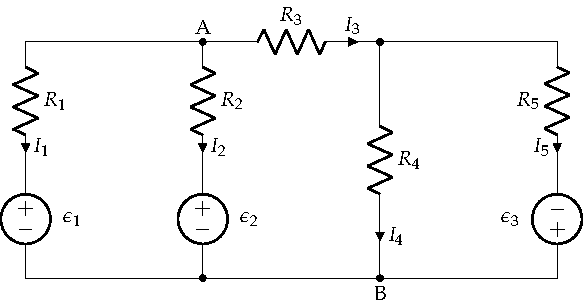
\includegraphics{figuras/mallas2.pdf}
\end{center}

\subsection*{Solución}
Se usan tres corrientes de malla con giro a derechas, de nombre (de
izquierda a derecha), $I_a$, $I_b$ e $I_c$. Escribiendo el sistema de
ecuaciones del método de las mallas en forma matricial:
\begin{equation*}
  \begin{bmatrix}
    2 & -1 & 0 \\
    -1 & 6 & -3 \\
    0 & -3 & 7
  \end{bmatrix}
  \cdot
  \begin{bmatrix}
    I_a\\
    I_b\\
    I_c
  \end{bmatrix}
  =
  \begin{bmatrix}
    -118\\
    236\\
    118
  \end{bmatrix}
\end{equation*}
cuya solución es:
\begin{align*}
  I_a &= \qty{-32}{\ampere}\\
  I_b &= \qty{54}{\ampere}\\
  I_c &= \qty{40}{\ampere}
\end{align*}

Estableciendo las relaciones entre las corrientes de rama y las
corrientes de malla, y sustituyendo, se llega a la conclusión de que:

\vspace{-4mm}
\begin{align*}
  I_1 &= -I_a=\qty{32}{\ampere}\\
  I_2 &= I_a - I_b=-32-54=\qty{-86}{\ampere}\\
  I_3 &= I_b=\qty{54}{\ampere}\\
  I_4 &= I_b - I_c=54-40=\qty{14}{\ampere}\\
  I_5 &= I_c=\qty{40}{\ampere}
\end{align*}

\emph{Se recomienda comprobar que estos resultados cumplen la 1LK en
  los nudos del circuito, para asegurarse de que la resolución es
  correcta.}

\vspace{4mm}
La diferencia de potencial entre A y B es:
\begin{equation*}
  U_{AB} = I_3 \cdot R_3 + I_4 \cdot R_4 = 54\cdot 2+14\cdot 3= \qty{150}{\volt}
\end{equation*}

La potencia entregada por los generadores del circuito es:

\vspace{-4mm}
\begin{align*}
  P_{\epsilon_1} &= \epsilon_1 \cdot (-I_1) = -\qty{3,776}{\kilo\watt}\\
  P_{\epsilon_2} &= \epsilon_2 \cdot (-I_2) = \qty{20,296}{\kilo\watt}\\
  P_{\epsilon_3} &= \epsilon_3 \cdot I_5 = \qty{4,72}{\kilo\watt}\\
  P_\epsilon &= P_{\epsilon_1} + P_{\epsilon_2} + P_{\epsilon_3} = \qty{21,24}{\kilo\watt}  
\end{align*}

Es importante recordar que el criterio de signos de un generador considera que la potencia entregada es positiva cuando la corriente sale del generador por su terminal positivo. Por tanto, $I_1$ e $I_2$ son empleadas con un signo negativo. En consecuencia, la potencia del generador $\epsilon_1$ es negativa, lo que quiere decir que este generador funciona como receptor (absorbe potencia). Ahora bien, dado que $I_2$ tiene valor negativo (es decir, circula en sentido contrario al indicado en la figura), la potencia del generador $\epsilon_2$ es positiva, de forma que este generador actúa como tal.

\vspace{3mm}
La potencia disipada por las resistencias es:

\vspace{-3mm}
\begin{align*}
  P_{R_1} &= I_1^2 \cdot R_1 = \qty{1,024}{\kilo\watt}\\
  P_{R_2} &= I_2^2 \cdot R_2 = \qty{7,396}{\kilo\watt}\\
  P_{R_3} &= I_3^2 \cdot R_3 = \qty{5,832}{\kilo\watt}\\
  P_{R_4} &= I_4^2 \cdot R_4 = \qty{588}{\watt}\\
  P_{R_5} &= I_5^2 \cdot R_5 = \qty{6,4}{\kilo\watt}\\
  P_R &= \sum_i P_{Ri} = \qty{21,24}{\kilo\watt}  
\end{align*}

Comprobamos que se cumple el balance de potencias.

%%%%%%%%%%%%%%%%%%%%%%%%%%%%%%%%%%%%%%%%%%%%%%%%%%%%%%%%%%%%%%%%%% 
\section{Enunciado}
En el circuito de la figura, se debe determinar:
\begin{itemize}
\item Todas las intensidades de rama señaladas.
\item Carga, polaridad y energía almacenada en los condensadores.
\item Balance de potencias.
\end{itemize}

  Datos: $ \; R_i = \qty[parse-numbers=false]{i}{\ohm}$; \; $C_i = \qty[parse-numbers=false]{i}{\micro\farad}$; \; $E_1 = \qty{8}{\volt}$; \; $E_2 = \qty{6}{\volt}$; \; $E_3 = \qty{4}{\volt}$

\begin{center}
  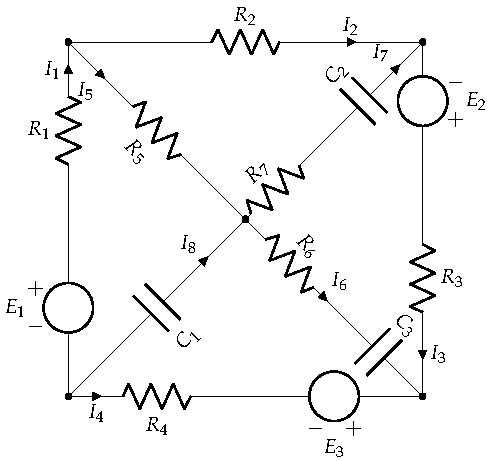
\includegraphics{figuras/BT1_09.pdf}
\end{center}


\subsection*{Solución}
Al tratarse de un circuito alimentado por corriente continua, los
condensadores se comportan como un circuito abierto, por lo que el
circuito a analizar es el mostrado en la figura.

\begin{center}
  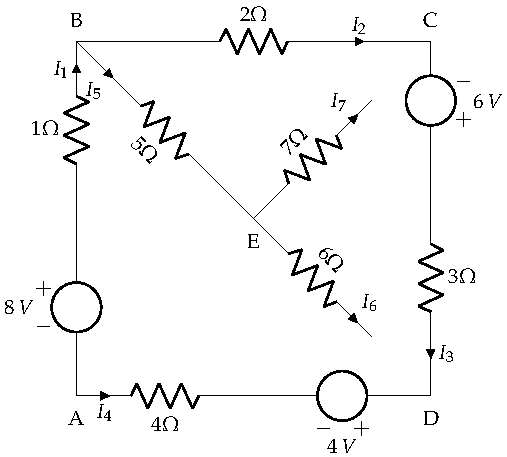
\includegraphics{figuras/BT1_09_sol.pdf}
\end{center}

Por simple observación, obtenemos:
\begin{equation*}
  I_5=I_6=I_7=\qty{0}{\ampere}
\end{equation*}
quedando una única malla por la que circula la misma corriente
$I_1=I_2=I_3=-I_4=I$. Por la 2LK, considerando que $I$ va en sentido
horario, se obtiene que:
\begin{equation*}
  -8+1\, I+2\,I-6+3\,I+4+4\,I=0 \quad \Rightarrow \quad {I = \dfrac{8+6-4}{1+2+3+4}=\qty{1}{\ampere}=I_1=I_2=I_3=-I_4}
\end{equation*}

Para determinar la carga de los condensadores hay que calcular las
tensiones en los diferentes nudos. Considerando $E$ como tierra:
\begin{align*}
  U_{AE}&=U_{A}-\cancelto{0}{U_{E}}=-8+1\,I_1+5\,I_5=-8+1\cdot 1 + 5\cdot 0=\qty{-7}{\volt}\\
  U_{CE}&=U_{C}-\cancelto{0}{U_{E}}=-2\,I_2+5\,I_5=-2\cdot 1+5\cdot 0 =\qty{-2}{\volt}\\
  U_{DE}&=U_{D}-\cancelto{0}{U_{E}}=4-4\, I_4-8+1\,I_1+5\,I_5=4-4\cdot (-1)-8+1\cdot 1 +5\cdot 0=\qty{1}{\volt}
\end{align*}
Con estas tensiones, se determina la carga de los condensadores:
\begin{align*}
  Q_{1\si{\micro\farad}} &= C_{1\si{\micro\farad}} \cdot U_{AE} = 1\cdot 10^{-6}\cdot (-7)=\qty{-7}{\micro\coulomb}\\
  Q_{2\si{\micro\farad}} &= C_{2\si{\micro\farad}} \cdot U_{CE} = 2\cdot 10^{-6}\cdot (-2)=\qty{-4}{\micro\coulomb}\\
  Q_{3\si{\micro\farad}} &= C_{3\si{\micro\farad}} \cdot U_{DE} = 3\cdot 10^{-6}\cdot 1=\qty{3}{\micro\coulomb}
\end{align*}
Aquellos condensadores en los que la carga es negativa, significa que
tienen la polaridad contraria a la considerada. La energía es:
\begin{align*}
  E_{1\si{\micro\farad}}&=\dfrac{1}{2}\,C_{1\si{\micro\farad}}\cdot U_{AE}^2 = \dfrac{1}{2}\cdot 1\cdot 10^{-6}\cdot (-7)^2 = \qty{24.5}{\micro\joule}\\
  E_{2\si{\micro\farad}}&=\dfrac{1}{2}\,C_{2\si{\micro\farad}}\cdot U_{CE}^2 = \dfrac{1}{2}\cdot 2\cdot 10^{-6}\cdot (-2)^2 = \qty{4}{\micro\joule}\\
  E_{3\si{\micro\farad}}&=\dfrac{1}{2}\,C_{3\si{\micro\farad}}\cdot U_{DE}^2 = \dfrac{1}{2}\cdot 3\cdot 10^{-6}\cdot 1^2 = \qty{1.5}{\micro\joule}
\end{align*}

Se calculan las potencias de los elementos activos y las potencias consumidas por las resistencias:
\begin{itemize}
\item Potencias de los elementos activos:
    \begin{align*}
      P_{E1} &= E_1 \cdot I_1 = \qty{8}{\watt}\\
      P_{E2} &= E_2 \cdot I_3 = \qty{6}{\watt}\\
      P_{E3} &= E_3 \cdot I_4 = -\qty{4}{\watt}
    \end{align*}
\item Potencias de las resistencias:
    \begin{align*}
      P_{R,1}&= R_1 \cdot I_1^2=1\cdot 1^2 = \qty{1}{\watt}\\
      P_{R,2}&= R_2 \cdot I_2^2=2\cdot 1^2 = \qty{2}{\watt}\\
      P_{R,3}&= R_3 \cdot I_3^2=3\cdot 1^2 = \qty{3}{\watt}\\
      P_{R,4}&= R_4 \cdot I_4^2=4\cdot (-1)^2 = \qty{4}{\watt}
    \end{align*}
\end{itemize}
Donde se cumple que la potencia total aportada por los generadores es igual a la potencia consumida por las resistencias.

%%%%%%%%%%%%%%%%%%%%%%%%%%%%%%%%%%%%%%%%%%%%%%%%%%%%%%%%%%%%%%%%%% 

\section{Enunciado}
Aplicar el método de los nudos en el circuito de la figura para
determinar:
\begin{itemize}
\item Los potenciales de los nudos A, B, C y D.
\item Las intensidades de corriente señaladas.
\item Carga, polaridad y energía almacenada en los condensadores,
  supuestos sin carga inicial.
\end{itemize}
Datos:
$ \; R_i = \qty[parse-numbers=false]{i}{\ohm}$; \; $C_i = \qty[parse-numbers=false]{i}{\micro\farad}$; \; $\epsilon_1 = \qty{6}{\volt}$; \; $\epsilon_2 =
\qty{18}{\volt}$; \; $\epsilon_3 = \qty{6}{\volt}$

\begin{center}
  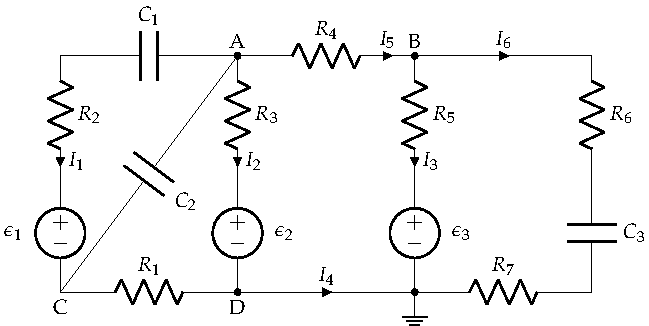
\includegraphics[]{figuras/nudos_condensadores.pdf}
\end{center}

\subsection*{Solución}

Sustituimos los condensadores por circuitos abiertos. En consecuencia, por las ramas correspondientes no puede circular corriente:

\vspace{2mm}
\begin{minipage}{0.65\linewidth}
  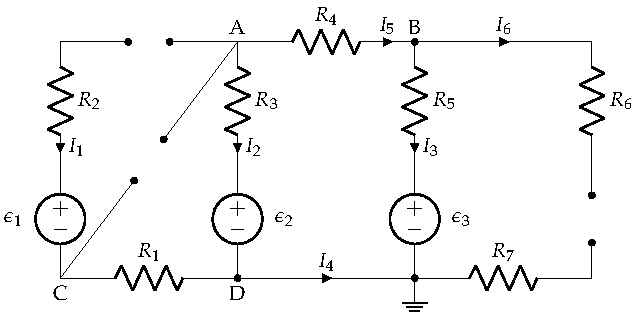
\includegraphics[scale=1]{figuras/nudos_condensadores2.pdf}
\end{minipage}
\begin{minipage}{0.25\linewidth}
    \begin{align*}
      I_1 &= \qty{0}{\ampere}\\
      I_6 &= \qty{0}{\ampere}
    \end{align*}    
\end{minipage}

\vspace{6mm}
Luego el circuito equivalente es:

\vspace{2mm}
\begin{minipage}{0.32\linewidth}
    \begin{center}
        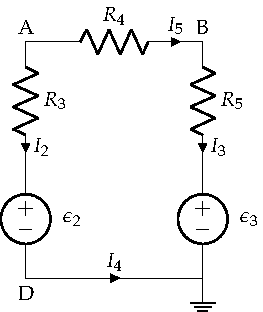
\includegraphics[scale=1]{figuras/nudos_condensadores3.pdf}
    \end{center}
\end{minipage}
\begin{minipage}[c]{0.08\linewidth}
    \begin{center}
    $\LARGE \xrightarrow{\hspace*{0.5cm}}$ % https://latex.org/forum/viewtopic.php?t=3894
    \end{center}
\end{minipage}    
\begin{minipage}{0.6\linewidth}
    \begin{center}
        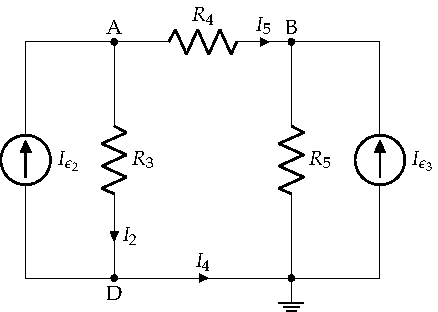
\includegraphics[scale=1]{figuras/nudos_condensadores4.pdf}
    \end{center}
\end{minipage}

\vspace{4mm}
Donde hemos transformado las fuentes de tensión en fuentes de corriente, para poder aplicar el método de los nudos.

\vspace{3mm}
Formulando la ecuación general del método de los nudos:

\begin{equation*}
  \begin{bmatrix}
    G_3 + G_4 & -G_4\\
    -G_4 & G_5 + G_4\\
  \end{bmatrix} \cdot %
  \begin{bmatrix}
    V_A\\
    V_B
  \end{bmatrix} = %
  \begin{bmatrix}
    \epsilon_2/R_3\\
    \epsilon_3/R_5
  \end{bmatrix}
\end{equation*}

\vspace{4mm}
Sustituyendo valores y resolviendo:

\vspace{-6mm}
\begin{align*}
  V_A &= \qty{15}{\volt}\\
  V_B &= \qty{11}{\volt}
\end{align*}

Además, $V_D = \qty{0}{\volt}$ , dado que está conectado a tierra. Por otra parte, la caída de tensión en la resistencia $R_1$ es de $\qty{0}{\volt}$, dado que $I_1 = \qty{0}{\ampere}$, luego $V_C = V_D = \qty{0}{\volt}$.

\vspace{4mm}

Con estos resultados podemos obtener los valores de las corrientes de rama. Volvemos al circuito original para plantear las ecuaciones de rama:

\vspace{-4mm}
\begin{align*}
  V_A &= I_2 \cdot R_3 + \epsilon_2\\
  V_B &= I_3 \cdot R_5 + \epsilon_3
\end{align*}

De estas ecuaciones despejamos $I_2$ e $I_3$. Además, teniendo en cuenta que $I_1 = I_6 = 0$, tenemos:

\vspace{-3mm}
\begin{align*}
  I_5 &= I_3\\
  I_4 &= I_2\\
  I_2 &= -I_3
\end{align*}

\vspace{-3mm}
En definitiva:

\vspace{-3mm}
\begin{align*}
  I_1 &= \qty{0}{\ampere}\\
  I_2 &= \qty{-1}{\ampere}\\
  I_3 &= \qty{1}{\ampere}\\
  I_4 &= \qty{-1}{\ampere}\\
  I_5 &= \qty{1}{\ampere}\\
  I_6 &= \qty{0}{\ampere}
\end{align*}

Finalmente, calculamos las diferencias de potencial en los
condensadores. En $C_1$ asignamos la polaridad positiva en A, y
tenemos:

\vspace{-2mm}
\begin{equation*}
  U_{AC} = U_{C_1} + \epsilon_1 \quad \rightarrow \quad U_{C_1} = \qty{9}{\volt}
\end{equation*}

\vspace{2mm}
Para $C_2$ y $C_3$, el cálculo es directo. Asignando la polaridad positiva en A y B, respectivamente:

\vspace{-4mm}
\begin{align*}
  U_{C_2} &=  U_{AC} = \qty{15}{\volt}\\
  U_{C_3} &=  U_{BD} = \qty{11}{\volt}
\end{align*}

\vspace{2mm}
En consecuencia, las cargas almacenadas en cada condensador son:

\vspace{-4mm}
\begin{align*}
  q_1 &= C_1 \cdot U_{C_1} = \qty{9}{\micro\coulomb}\\
  q_2 &= C_2 \cdot U_{C_2} = \qty{30}{\micro\coulomb}\\
  q_3 &= C_3 \cdot U_{C_3} = \qty{33}{\micro\coulomb}
\end{align*}

Y las energías almacenadas:

\vspace{-4mm}
\begin{align*}
  E_{C_1} &= \frac{1}{2} \cdot C_1 \cdot (U_{C_1})^2 = \qty{40.5}{\micro\joule}\\
  E_{C_2} &= \frac{1}{2} \cdot C_2 \cdot (U_{C_2})^2 = \qty{225}{\micro\joule}\\
  E_{C_3} &= \frac{1}{2} \cdot C_3 \cdot (U_{C_3})^2 = \qty{181.5}{\micro\joule}
\end{align*}

%%%%%%%%%%%%%%%%%%%%%%%%%%%%%%%%%%%%%%%%%%%%%%%%%%%%%%%%%%%%%%%%%% 

\section{Enunciado}

En el circuito de la figura, donde se sabe que la carga inicial de los
condensadores era de $\qty{10}{\micro\coulomb}$ para $C_1$ y de
$\qty{20}{\micro\coulomb}$ para $C_2$, con las polaridades indicadas,
se pide determinar:
\begin{itemize}
\item Intensidades de corriente señaladas.
\item Potenciales en los puntos A, B, C, D, E y F.
\end{itemize}

Datos:
$\; \epsilon_1=\qty{90}{\volt};\; \epsilon_2=\qty{60}{\volt};\;
\epsilon_3=\qty{30}{\volt};\; R_{1}= R_2 = R_3 =
\qty{10}{\ohm};\; R_{4}= R_5 = \qty{30}{\ohm};\; C_{1}=
\qty{10}{\micro\farad};\; C_{2}= \qty{20}{\micro\farad};\; L_1 =
\qty{1}{\micro\henry}$

\begin{center}
  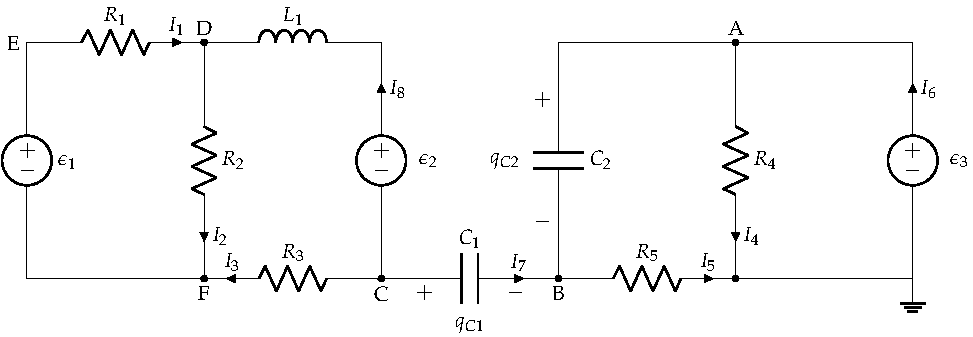
\includegraphics[scale = 0.9]{figuras/mallas_carga_inicial.pdf}
\end{center}


\subsection*{Solución}

Sustituimos los condensadores por circuitos abiertos, lo que implica que por las ramas correspondientes no puede circular corriente:

\vspace{-4mm}
\begin{align*}
  I_5 &= \qty{0}{\ampere}\\
  I_7 &= \qty{0}{\ampere}
\end{align*}

\begin{center}
  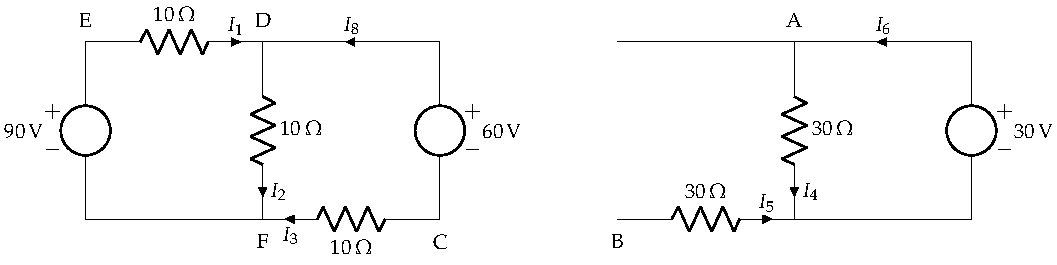
\includegraphics[width=\linewidth]{figuras/BT1_10_mod.pdf}
\end{center}

En consecuencia:

\vspace{-4mm}
\begin{align*}
  I_3 &= -I_8\\
  I_4 &= I_6
\end{align*}

\vspace{2mm}
Además, la bobina $L_1$ se sustituye por un cortocircuito.

\vspace{3mm}
Dado que el circuito original está ``partido'' en dos porciones inconexas, podemos analizar de manera independiente cada una de las dos porciones. Si aplicáramos la ecuación general de mallas al circuito en su conjunto, obtendríamos una matriz con ceros en los elementos comunes entre la malla 3 (malla en la que se incluye el generador 3), y las mallas 1 y 2, por lo que el sistema de ecuaciones $3\times 3$ sería separable en dos partes (de dimensiones $2\times 2$ y $1\times 1$).

\vspace{5mm}
Por lo tanto, en el circuito de la izquierda se tienen dos mallas, considerando las corrientes de malla mostradas en la siguiente figura:

\begin{center}
  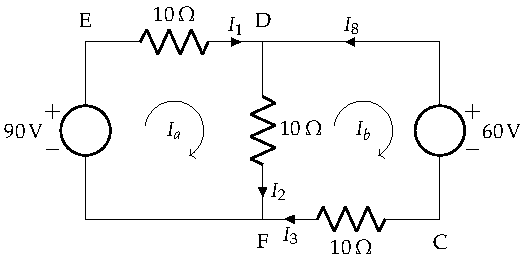
\includegraphics{figuras/BT1_10_izq_mallas.pdf}
\end{center}


\begin{equation*}
  \begin{bmatrix}
    R_1 + R_2 & -R_2\\
    -R_2 & R_2 + R_3\\
  \end{bmatrix} \cdot %
  \begin{bmatrix}
    I_a\\
    I_b
  \end{bmatrix} = %
  \begin{bmatrix}
    \epsilon_1\\
    -\epsilon_2
  \end{bmatrix}
\end{equation*}

\vspace{2mm}
La solución de este sistema es:

\vspace{-4mm}
\begin{align*}
  I_a &= \qty{4}{\ampere}\\
  I_b &= \qty{-1}{\ampere}
\end{align*}

\vspace{-4mm}
siendo,

\vspace{-4mm}
\begin{align*}
  I_1 &= I_a\\
  I_2 &= I_a - I_b\\
  I_3 &= I_b\\
  I_8 &= -I_b
\end{align*}

En el circuito de la derecha tenemos una única malla:

\begin{equation*}
  \epsilon_3 = I_4 \cdot R_4 \rightarrow I_4 = \qty{1}{\ampere}
\end{equation*}

Por tanto:
\begin{align*}
  I_1 &= \qty{4}{\ampere}\\
  I_2 &= \qty{5}{\ampere}\\
  I_3 &= \qty{-1}{\ampere}\\
  I_4 &= \qty{1}{\ampere}\\
  I_5 &= \qty{0}{\ampere}\\
  I_6 &= \qty{1}{\ampere}\\
  I_7 &= \qty{0}{\ampere}\\
  I_8 &= \qty{1}{\ampere}\\
\end{align*}

Para calcular los potenciales en los puntos A y B:

\vspace{-3mm}
\begin{align*}
  V_A &= \epsilon_3 = \qty{30}{\volt}\\
  V_B &= R_5 \cdot I_5 = \qty{0}{\volt}
\end{align*}

Para calcular el potencial en el punto C, debemos tener en cuenta que el condensador $C_1$ conserva su carga inicial porque el circuito no está cerrado en la parte superior. Por tanto:

\begin{equation*}
  U_{CB} = U_{C_1} = \frac{q_{C_1,0}}{C_1} = \qty{1}{\volt}
\end{equation*}
(para comprobar que nunca circula corriente por un elemento que esté conectado como $C_1$, se puede aplicar 1LK en los nudos D, F, y C, y sumando las 3 ecs. se obtiene que $I_7 = 0$)

\vspace{3mm}
Luego:

\vspace{-3mm}
\begin{equation*}
  U_C = U_{CB} + U_B = \qty{1}{\volt}
\end{equation*}

\vspace{2mm}
A partir de este resultado, podemos calcular el resto de potenciales:

\vspace{-3mm}
\begin{align*}
  U_D &= U_{DC} + U_C = \epsilon_2 + U_C = \qty{61}{\volt}\\
  U_E &= U_{ED} + U_D = I_1 \cdot R_1 + U_D = \qty{101}{\volt}\\
  U_F &= U_{FC} + U_C = -I_3 \cdot R_3 + U_C = \qty{11}{\volt}
\end{align*}

%%%%%%%%%%%%%%%%%%%%%%%%%%%%%%%%%%%%%%%%%%%%%%%%%%%%%%%%%%%%%%%%%% 
\section{Enunciado}
En el circuito de la figura, los condensadores se conectaron sin
carga. Mediante el método de las mallas, se pide determinar:
\begin{itemize}
\item Intensidades de corriente señaladas.
\item Potenciales en los puntos A, B, C y D.
\item Polaridades, cargas, y energías de los condensadores.
\item Balance de potencias.
\end{itemize}
\begin{minipage}[c]{0.2\linewidth}
  \begin{align*}
    \epsilon_{1}&=\qty{118}{\volt}\\
    \epsilon_{2}&=\qty{236}{\volt}\\
    \epsilon_{3}&=\qty{118}{\volt}\\
    R_{1}&= \qty{4}{\ohm}\\
    R_{2}&=R_{3}=\qty{1}{\ohm}\\
    R_{4}&= \qty{3}{\ohm}\\
    R_{5}&= \qty{2}{\ohm}\\
    C_{1}&=C_{2}=C_{3}=\qty{2}{\micro\farad}\\
    L_1 &= L_2 = L_3 = \qty{1}{\milli\henry}\\
  \end{align*}
\end{minipage}
\begin{minipage}[c]{0.8\linewidth}
  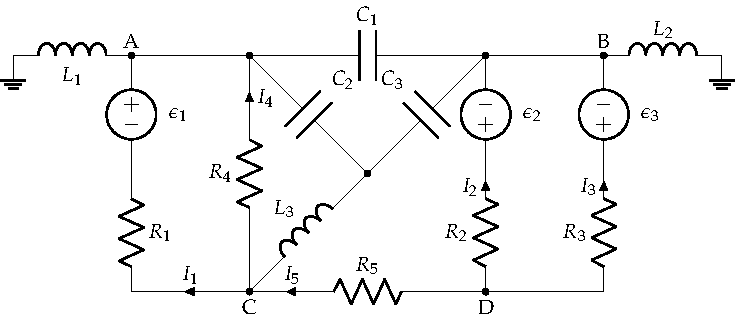
\includegraphics{figuras/mallas_condensadores.pdf}
\end{minipage}

\subsection*{Solución}
Se sustituyen los condensadores y las bobinas por sus equivalentes en un circuito de corriente continua (circuito abierto y cortocircuito, respectivamente). Por otro lado, dado que hay dos tomas de tierra en el esquema, esto no implica que haya dos referencias de potencial distintas: simplemente indica que esos dos puntos están cortocircuitados. En el circuito resultante, se definen tres corrientes de malla, como se muestra en el circuito de la figura:

\begin{center}            
    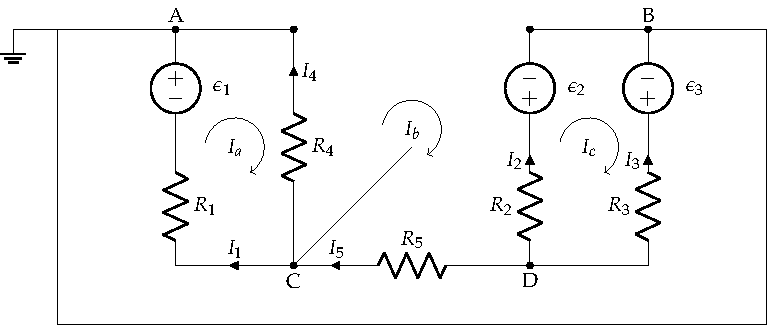
\includegraphics{figuras/mallas_condensadores_sol.pdf}
\end{center}
(la malla $b$ puede definirse de esta forma porque los puntos A y B están cortocircuitados)

\vspace{4mm}
Usamos la ecuación general del método de mallas:    
\begin{equation*}
    \begin{bmatrix}
        R_1 + R_4 & -R_4 & 0\\
        -R_4 & R_4 + R_5 + R_2 & -R_{2}\\
        0 & -R_2 & R_2 + R_3
    \end{bmatrix} \cdot %
    \begin{bmatrix}
        I_{a}\\
        I_{b}\\
        I_{c}
    \end{bmatrix} = %
    \begin{bmatrix}
        \epsilon_1\\
        \epsilon_2\\
        \epsilon_3 - \epsilon_2
    \end{bmatrix}
\end{equation*} 

\begin{equation*}
    \begin{bmatrix}
        7 & -3 & 0\\
        -3 & 6 & -1\\
        0 & -1 & 2
    \end{bmatrix} \cdot %
    \begin{bmatrix}
        I_{a}\\
        I_{b}\\
        I_{c}
    \end{bmatrix} = %
    \begin{bmatrix}
        118\\
        236\\
        -118
    \end{bmatrix}
\end{equation*}  

Cuya solución es:

\vspace{-6mm}
\begin{eqnarray*}
I_a & = & \qty{40}{\ampere}\\
I_b & = & \qty{54}{\ampere}\\
I_c & = & -\qty{32}{\ampere}
\end{eqnarray*}

Por tanto, las corrientes indicadas en el circuito son:

\vspace{-4mm}
\begin{eqnarray*}
I_1 & = & \qty{40}{\ampere}\\
I_2 & = & \qty{-86}{\ampere}\\
I_3 & = &  \qty{32}{\ampere}\\
I_4 & = &  \qty{14}{\ampere}\\
I_5 & = &  \qty{54}{\ampere}
\end{eqnarray*}

Los potenciales en los puntos indicados son:

\vspace{-4mm}
\begin{align*}
V_A &= \qty{0}{\volt}\\
V_B &= \qty{0}{\volt}\\
V_C &= I_4 \cdot R_4 = \qty{42}{\volt}\\
V_D &= I_5 \cdot R_5 + V_C = \qty{150}{\volt}\\
\end{align*}

\vspace{-2mm}
Por tanto, las polaridades de los condensadores y sus valores de tensión son los siguientes:

\vspace{-3mm}
\begin{eqnarray*}
    U_{C_1} = U_{BA} & = & \qty{0}{\volt}\\
    q_1 = C_1 \cdot U_{C_1} & = & \boxed{\qty{0}{\coulomb}}\\
    E_{C_1} = \frac{1}{2} C_1 \cdot (U_{C_1})^2 & = & \boxed{\qty{0}{\joule}}
\end{eqnarray*}

\vspace{-4mm}
\begin{eqnarray*}
    U_{C_2} = U_{CA} & = & \qty{42}{\volt}\\
    q_2 = C_2 \cdot U_{C_2} & = & \boxed{\qty{84}{\micro\coulomb}}\\
    E_{C_2} = \frac{1}{2} C_2 \cdot (U_{C_2})^2 & = & \boxed{\qty{1.76}{\milli\joule}}
\end{eqnarray*}

\vspace{-4mm}
\begin{eqnarray*}
    U_{C_3} = U_{CB} & = & \qty{42}{\volt}\\
    q_3 = C_3 \cdot U_{C_3} & = & \boxed{\qty{84}{\micro\coulomb}}\\
    E_{C_3} = \frac{1}{2} C_3 \cdot (U_{C_3})^2 & = & \boxed{\qty{1.76}{\milli\joule}}
\end{eqnarray*}

\vspace{5mm}
Finalmente, podemos formular el balance de potencias como potencia entregada por los elementos activos frente a potencia consumida por los elementos pasivos:

\vspace{1mm}
\begin{itemize}
    \item La potencia total entregada por los elementos activos es $\qty{21240}{\watt}$:
\end{itemize}

\vspace{-7mm}
\begin{eqnarray*}
P_{\epsilon_1} = \epsilon_1 \cdot I_1 & = & \qty{4720}{\watt}\\
P_{\epsilon_2} = \epsilon_2 \cdot (-I_2) & = & \qty{20296}{\watt}\\
P_{\epsilon_3} = \epsilon_3 \cdot (-I_3) & = & \qty{-3776}{\watt}
\end{eqnarray*}

\vspace{0.5mm}
\begin{itemize}
    \item La potencia total consumida por los elementos pasivos también es $\qty{21240}{\watt}$:
\end{itemize}

\vspace{-6mm}
\begin{eqnarray*}
P_{R_1} = R_1 \cdot (I_1)^2 & = & \qty{6400}{\watt}\\
P_{R_2} = R_2 \cdot (I_2)^2 & = & \qty{7396}{\watt}\\
P_{R_3} = R_3 \cdot (I_3)^2 & = & \qty{1024}{\watt}\\
P_{R_4} = R_4 \cdot (I_4)^2 & = & \qty{588}{\watt}\\
P_{R_5} = R_5 \cdot (I_5)^2 & = & \qty{5832}{\watt}
\end{eqnarray*}

%%%%%%%%%%%%%%%%%%%%%%%%%%%%%%%%%%%%%%%%%%%%%%%%%%%%%%%%%%%%%%%%%% 
\section{Enunciado}
En el circuito de la figura, determinar:
\begin{itemize}
\item Las ecuaciones para el cálculo de las intensidades.
\item Todas las intensidades indicadas.
\item Potenciales en todos los nudos.
\item Carga y energía almacenada en los condensadores.
\end{itemize}

\vspace{2mm}
  Datos: $R_1 = \qty{2}{\ohm}$; $R_2 = \qty{4}{\ohm}$; $R_3 = \qty{2}{\ohm}$; $R_4 = \qty{1}{\ohm}$; $R_5 = \qty{2}{\ohm}$; $R_6 = \qty{1}{\ohm}$; $E_1 = \qty{8}{\volt}$; $E_2 = \qty{8}{\volt}$; $C_i = \qty[parse-numbers=false]{i}{\micro\farad}$

\begin{center}
  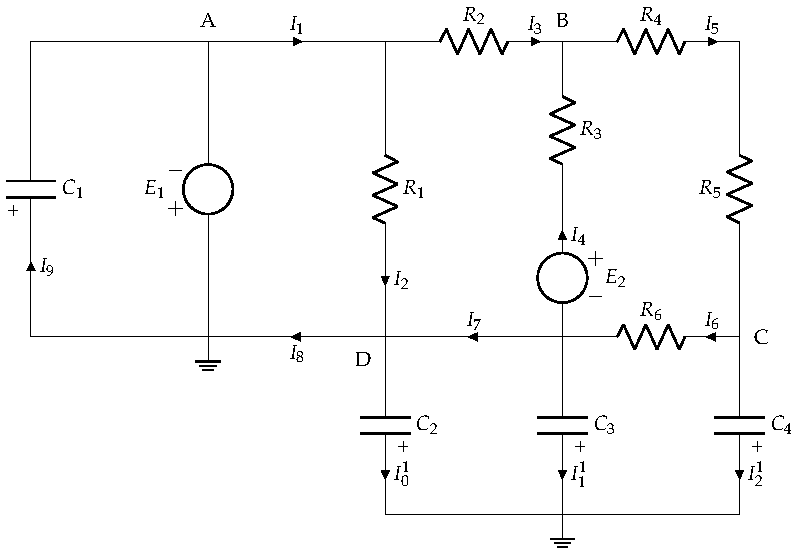
\includegraphics{figuras/BT1_11.pdf}
\end{center}

\subsection*{Solución}
Al tratarse de alimentación en CC, se sustituyen los condensadores por
circuitos abiertos, quedando el circuito de la figura:
\begin{center}
  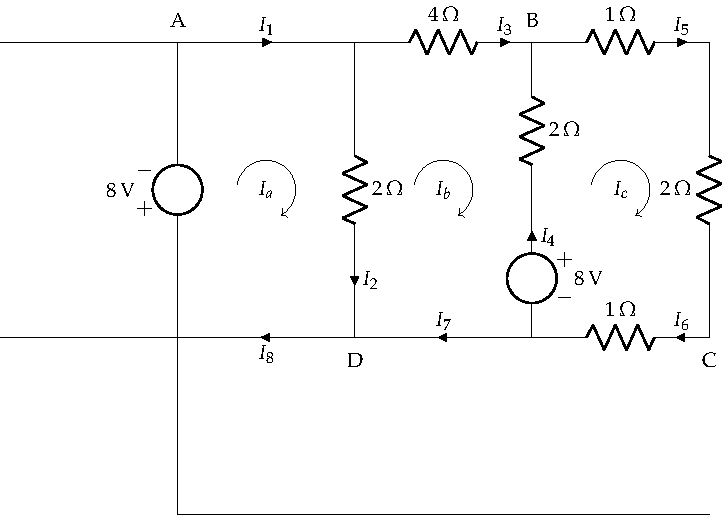
\includegraphics{figuras/BT1_11_mod.pdf}
\end{center}

Aplicando el método de mallas, con las corrientes indicadas, se
plantea el sistema de ecuaciones en forma matricial:
\begin{equation*}
  \begin{bmatrix}
    2 & -2 & 0 \\
    -2 & 8 & -2 \\
    0 & -2 & 6
  \end{bmatrix} \cdot
  \begin{bmatrix}
    I_a\\
    I_b\\
    I_c
  \end{bmatrix} = %
  \begin{bmatrix}
    -8 \\
    -8\\
    8
  \end{bmatrix}
\end{equation*}

\vspace{2mm}
Las ecuaciones completas para calcular las intensidades son:
\begin{align*}
  2\,I_a&-2\,I_b = -8\\
  -2\,I_a&+8\,I_b-2\,I_c = -8\\
  -2\,I_b&+ 6\,I_c = 8
\end{align*}
Cuya solución es:
\begin{align*}
  I_a&=\qty{-6.5}{\ampere}\\
  I_b&=\qty{-2.5}{\ampere}\\
  I_c&=\qty{0.5}{\ampere}\\
\end{align*}

Estableciendo las relaciones entre las corrientes de malla y las de rama del circuito:
\begin{align*}
  I_1&=I_8=I_a= \boxed{\qty{-6.5}{\ampere}}\\
  I_2&=I_a-I_b=-6.5-(-2.5)= \boxed{\qty{-4}{\ampere}}\\
  I_3&=I_7=I_b= \boxed{\qty{-2.5}{\ampere}}\\
  I_4&=I_c-I_b=0.5-(-2.5)= \boxed{\qty{3}{\ampere}}\\
  I_5&=I_6=I_c= \boxed{\qty{0.5}{\ampere}}\\
\end{align*}

\vspace{-2mm}
Una forma alternativa de resolver el circuito consiste en reparar en que $E_1$ es generador dominante, por lo que puede determinarse directamente el valor de $I_2 = - E_1 / R_1 = -4\si{\ampere}$. Esto permite usar únicamente 2 mallas, lo que reduce el sistema de ecuaciones a $2\times 2$: 

\vspace{4mm}
\begin{minipage}{0.6\linewidth}
    \begin{center}
    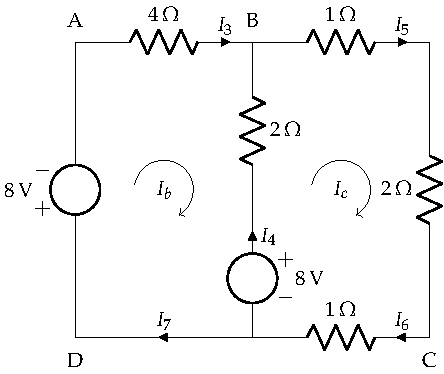
\includegraphics[scale=1]{figuras/BT1_11_mod2.pdf}
    \end{center}
\end{minipage}
\hfill
\begin{minipage}{0.3\linewidth}
    \begin{equation*}
      \begin{bmatrix}
        6 & -2  \\
        -2 & 6
      \end{bmatrix} \cdot
      \begin{bmatrix}
        I_b\\
        I_c
      \end{bmatrix} = %
      \begin{bmatrix}
        -16\\
        8
      \end{bmatrix}
    \end{equation*}

    \vspace{6mm}
    
    Cuya solución es la misma que 
    
    la obtenida anteriormente.
\end{minipage}

\vspace{4mm}
Conociendo las corrientes y teniendo el nudo de tierra como referencia, se calculan los potenciales:
\begin{align*}
  U_A&=-U_{8\si{\volt}}= \boxed{\qty{-8}{\volt}}\\
  U_B&=-U_{R2\Omega}+U_{8\si{\volt}}=-2\cdot 3+8= \boxed{\qty{2}{\volt}}\\
  U_C&=U_{R1\Omega}=1\cdot 0.5= \boxed{\qty{0.5}{\volt}}\\
  U_D&= \boxed{\qty{0}{\volt}}
\end{align*}

\vspace{4mm}
Con los potenciales, se determina la carga de los condensadores:
\begin{align*}
  Q_{1\si{\micro\farad}}&=C_{1\si{\micro\farad}}\, (-U_{A}) = 1\cdot 10^{-6}\cdot (-(-8))= \boxed{\qty{8}{\micro\coulomb}}\\
  Q_{2\si{\micro\farad}}&=C_{2\si{\micro\farad}} \cdot \qty{0}{\volt} = \boxed{\qty{0}{\micro\coulomb}}\\
  Q_{3\si{\micro\farad}}&=C_{3\si{\micro\farad}} \cdot \qty{0}{\volt} = \boxed{\qty{0}{\micro\coulomb}}\\
  Q_{4\si{\micro\farad}}&=C_{4\si{\micro\farad}}\, (-U_C) = 4\cdot 10^{-6}\cdot (-0.5)= \boxed{\qty{-2}{\micro\coulomb}}
\end{align*}

\vspace{4mm}
Aquellos condensadores en los que la carga es negativa, significa que tienen polaridad contraria a la considerada. La energía almacenada en cada uno de ellos es:

\begin{align*}
  E_{1\si{\micro\farad}}&=\dfrac{1}{2}\,C_{1\si{\micro\farad}}\cdot (-U_{A})^2 = \dfrac{1}{2}\cdot 1\cdot 10^{-6}\cdot (-(-8))^2= \boxed{\qty{32}{\micro\joule}}\\
  E_{2\si{\micro\farad}}&= \boxed{\qty{0}{\micro\joule}}\\
  E_{3\si{\micro\farad}}&= \boxed{\qty{0}{\micro\joule}}\\
  E_{4\si{\micro\farad}}&=\dfrac{1}{2}\,C_{4\si{\micro\farad}}\cdot (-U_{C})^2 = \dfrac{1}{2}\cdot 4\cdot 10^{-6}\cdot (-0.5)^2= \boxed{\qty{0.5}{\micro\joule}}
\end{align*}

%%%%%%%%%%%%%%%%%%%%%%%%%%%%%%%%%%%%%%%%%%%%%%%%%%%%%%%%%%%%%%%%%%
\section{Enunciado}
En el circuito de la figura se debe determinar:
\begin{itemize}
\item Las corrientes señaladas.
\item El balance de potencias, diferenciando entre elementos activos y
  elementos pasivos.
\item Los potenciales en los puntos A, B y C.
\item La carga y polaridad en los condensadores, supuestos sin carga
  inicial.
\end{itemize}
\begin{minipage}[c]{0.25\linewidth}
  \begin{align*}
    \epsilon_1&=\qty{1}{\volt}\\
    \epsilon_2&=\qty{7}{\volt}\\
    R_i &= \qty{1}{\ohm}\\
    C_i &= \qty[parse-numbers=false]{i}{\micro\farad}
  \end{align*}
\end{minipage}
\begin{minipage}[c]{0.75\linewidth}
  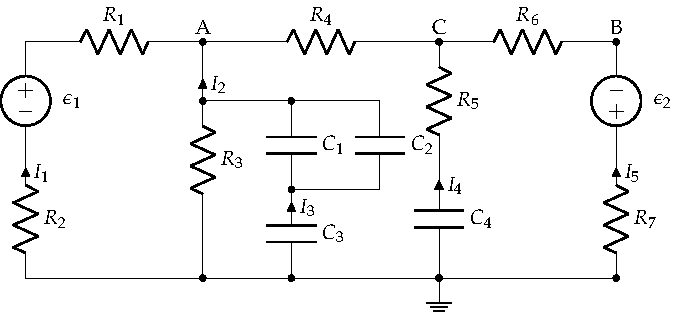
\includegraphics{figuras/mallas_agrupacion_condensadores.pdf}
\end{minipage}

\subsection*{Solución}
Sustituimos los condensadores por circuitos abiertos. En consecuencia, por las ramas correspondientes no puede circular corriente:

\vspace{-4mm}
\begin{align*}
  I_3 &= \boxed{\qty{0}{\ampere}}\\
  I_4 &= \boxed{\qty{0}{\ampere}}
\end{align*}

Tenemos dos mallas, y definimos dos corrientes de malla dextrógiras (sentido horario):

\begin{equation*}
  \begin{bmatrix}
    R_1 + R_2 + R_3 & -R_3\\
    -R_3 & R_3 + R_4 + R_6 + R_7\\
  \end{bmatrix} \cdot %
  \begin{bmatrix}
    I_a\\
    I_b
  \end{bmatrix} = %
  \begin{bmatrix}
    \epsilon_1\\
    \epsilon_2
  \end{bmatrix}
\end{equation*}

\vspace{3mm}
La solución de este sistema es:

\vspace{-5mm}
\begin{align*}
  I_a &= \qty{1}{\ampere}\\
  I_b &= \qty{2}{\ampere}
\end{align*}

\vspace{-1mm}
siendo,

\vspace{-5mm}
\begin{align*}
  I_1 &= I_a = \boxed{\qty{1}{\ampere}}\\
  I_2 &= I_b - I_a = \boxed{\qty{1}{\ampere}}\\
  I_5 &= -I_b = \boxed{\qty{-2}{\ampere}}
\end{align*}

\vspace{2mm}
La potencia de los dos elementos activos es:

\vspace{-4mm}
\begin{align*}
  P_{\epsilon1} = \epsilon_1 \cdot I_1 = \qty{1}{\watt}\\
  P_{\epsilon2} = \epsilon_2 \cdot (-I_5) = \qty{14}{\watt}
\end{align*}

En total, $P_\epsilon = \boxed{\qty{15}{\watt}}$

\vspace{3mm}
Aplicando la ley de Joule en cada resistencia comprobaríamos que la potencia total disipada en las resistencias del circuito coincide con los $\qty{15}{\watt}$.

\vspace{4mm}
Los potenciales en los puntos indicados son:

\vspace{-3mm}
\begin{align*}
  V_A &= -I_2 \cdot R_3 = \qty{-1}{\volt}\\
  V_B &= -\epsilon_2 - I_5 \cdot R_7 = \qty{-5}{\volt}\\
  V_C &= U_{CB} + V_B = -I_5 \cdot R_6 + V_B = \qty{-3}{\volt}
\end{align*}

\vspace{2mm}
La carga almacenada en el condensador $C_4$ se calcula con la ecuación:
\begin{equation*}
  q_4 = C_4 \cdot U_{C4} = C_4 \cdot (-U_C) = \qty{12}{\micro\coulomb}
\end{equation*}
donde se ha asignado la polaridad positiva en la conexión a tierra.

\vspace{4mm}
Los condensadores $C_1$, $C_2$ y $C_3$ forman parte de una asociación. Los condensadores $C_1$ y $C_2$ están asociados en paralelo:
\begin{equation*}
  C_{12} = C_1 \parallel C_2 = C_1 + C_2 = \qty{3}{\micro\farad}
\end{equation*}

\vspace{2mm}
A su vez, están conectados en serie con el condensador $C_3$:

\begin{equation*}
  C_T = \frac{C_{12} \cdot C_3}{C_{12} + C_3} = \qty{1.5}{\micro\farad}
\end{equation*}

\vspace{2mm}
Este condensador equivalente está conectado entre A y tierra, y asignamos la polaridad positiva a la conexión a tierra. Por tanto:

\vspace{-2mm}
\begin{equation*}
  U_{C_T} = -U_A = \qty{1}{\volt} \quad \rightarrow \quad q_T = C_T \cdot U_{C_T} = \qty{1.5}{\micro\coulomb}
\end{equation*}

\vspace{2mm}
Al tratarse de una conexión serie, esta carga es la misma que tienen el condensador $C_3$ y el condensador equivalente $C_{12}$.

\vspace{-7mm}
\begin{align*}
  q_3 &=  \boxed{\qty{1.5}{\micro\coulomb}}\\
  q_{12} &=  \qty{1.5}{\micro\coulomb}
\end{align*}

Con estas cargas podemos calcular las diferencias de potencial en estos condensadores:

\vspace{-4mm}
\begin{align*}
  U_{C3} &=  \frac{q_3}{C_3} = \qty{0.5}{\volt}\\
  U_{C12} &=  \frac{q_{12}}{C_{12}} = \qty{0.5}{\volt}
\end{align*}

Por tanto:

\vspace{-5mm}
\begin{align*}
  q_1 &= C_1 \cdot U_{C12} = \boxed{\qty{0.5}{\micro\coulomb}}\\
  q_2 &= C_2 \cdot U_{C12} = \boxed{\qty{1}{\micro\coulomb}}
\end{align*}

Comprobamos que $q_1 + q_2 = q_{12}$.
%%%%%%%%%%%%%%%%%%%%%%%%%%%%%%%%%%%%%%%%%%%%%%%%%%%%%%%%%%%%%%%%%%
\section{Enunciado}
El circuito de la figura está funcionando en régimen estacionario. Los
condensadores estaban inicialmente descargados. Resuelve el circuito
mediante el método que consideres conveniente para obtener los
siguientes resultados:
\begin{itemize}
\item Las intensidades señaladas.
\item Polaridad y energía almacenada en los condensadores.
\item Balance de potencias.
\end{itemize}
Datos:
$ \quad \epsilon_{1}=\qty{40}{\volt}; \quad \epsilon_{2}=\qty{22}{\volt}; \quad \epsilon_{3}=\qty{20}{\volt}; \quad
C_{1}=C_{2}=C_{3}=\qty{2}{\micro\farad}; \quad R_{g1}=R_{g2}=R_{g3}=\qty{4}{\ohm}; 
\\
\hspace*{14mm} R_{1}=R_{2}=R_{3}=R_{4}=\qty{2}{\ohm}; \quad R_{5}=R_{6}=R_{7}=\qty{1}{\ohm}$


\begin{center}
  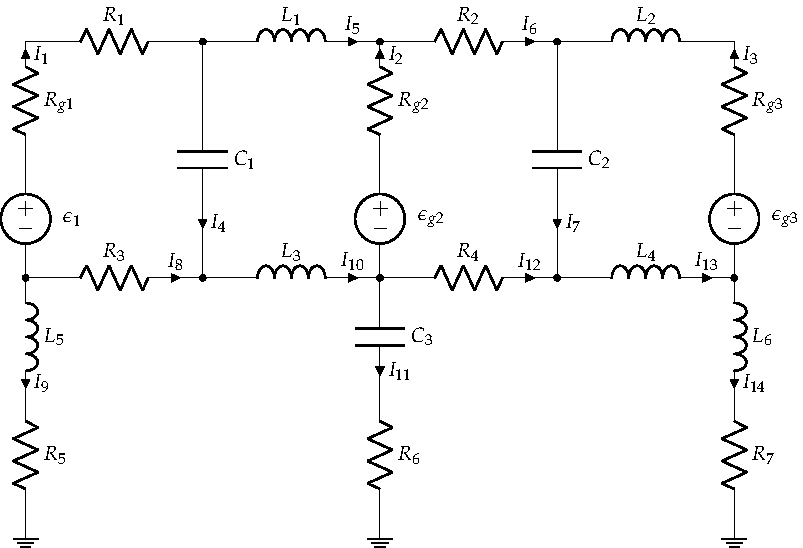
\includegraphics{figuras/mallas_condensadores_bobinas.pdf}
\end{center}


\subsection*{Solución}
Los condensadores se sustituyen por circuitos abiertos (inicialmente
están descargados) y las bobinas por cortocircuitos. De esta forma, el
circuito original queda reducido a tres mallas, como se muestra en la
siguiente figura:

\begin{center}
  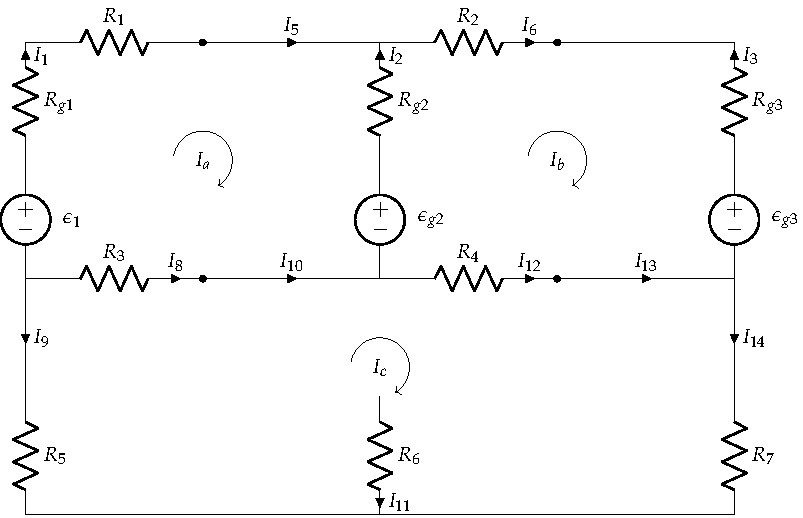
\includegraphics{figuras/mallas_condensadores_bobinas_mod.pdf}
\end{center}


Se resuelve mediante el método de mallas, cuyo sistema de ecuaciones
en forma matricial es:
\begin{equation*}
  \begin{bmatrix}
    12 & -4 & -2 \\
    -4 & 12 & -2\\
    -2 & -2 & 6
  \end{bmatrix}
  \cdot\begin{bmatrix}
         I_a\\
         I_b\\
         I_c
       \end{bmatrix}
       =
       \begin{bmatrix}
         18\\
         2\\
         0
       \end{bmatrix}
     \end{equation*}
     cuya solución es:
     \begin{align*}
       I_{a} & =  \qty{2}{\ampere}\\
       I_{b} & =  \qty{1}{\ampere}\\
       I_{c} & =  \qty{1}{\ampere}
     \end{align*}
     Relacionando estas corrientes de malla con las corrientes de rama
     señaladas en el circuito original (teniendo en cuenta que las
     corrientes que circulan por ramas con condensadores son nulas):
     \begin{align*}
       I_{1} & =  I_{a} = \qty{2}{\ampere}\\
       I_{2} & =  -I_{a}+I_{b} = \qty{-1}{\ampere}\\
       I_{3} & =  -I_{b} = \qty{-1}{\ampere}\\
       I_{4} & =  \qty{0}{\ampere}\\
       I_{5} & =  I_{a} = \qty{2}{\ampere}\\
       I_{6} & =  I_{b} = \qty{1}{\ampere}\\
       I_{7} & =  \qty{0}{\ampere}\\
       I_{8} & =  -I_{a}+I_{c} = \qty{-1}{\ampere}\\
       I_{9} & =  -I_{c} = \qty{-1}{\ampere}\\
       I_{10} & = -I_{a}+I_{c} = \qty{-1}{\ampere}\\
       I_{11} & =  \qty{0}{\ampere}\\
       I_{12} & =  -I_{b}+I_{c} = \qty{0}{\ampere}\\
       I_{13} & =  -I_{b}+I_{c} = \qty{0}{\ampere}\\
       I_{14} & =  I_{c} = \qty{1}{\ampere}
     \end{align*}

     El condensador $C_{1}$ está conectado directamente a la rama
     compuesta por la fuente $E_{2}$ y su resistencia $E_{g2}$ (debido
     a que la bobina se comporta como un cortocircuito). Por tanto,
     suponiendo que la polaridad positiva de este condensador
     corresponde a su borne superior, la tensión de este condensador
     es:
     \begin{equation*}
       U_{C1} = E_{2}-I_{2}\cdot R_{g2} = 22-(-1)\cdot4 = \qty{26}{\volt}
     \end{equation*}
     siendo correcta la polaridad asignada por el signo positivo de
     este resultado. La energía almacenada por el condensador es:
     \begin{equation*}
       E_{C1} = 1/2\cdot V_{C1}^{2}\cdot C_{1} = \qty{0.676}{\milli\joule}
     \end{equation*}

     El condensador $C_{2}$ está conectado directamente a la rama
     compuesta por la fuente $E_{3}$ y su resistencia $E_{g3}$ (debido
     a que la bobina se comporta como un cortocircuito). Por tanto,
     suponiendo que la polaridad positiva de este condensador
     corresponde a su borne superior, la tensión de este condensador
     es:
     \begin{equation*}
       U_{C2} = E_{3}-I_{3}\cdot R_{g3} = 20-(-1)\cdot4 = \qty{24}{\volt}
     \end{equation*}
     siendo correcta la polaridad asignada por el signo positivo de
     este resultado. La energía almacenada por el condensador es:
     \begin{equation*}
       E_{C2} = 1/2\cdot U_{C2}^{2}\cdot C_{2} = \qty{0.576}{\milli\joule}
     \end{equation*}

     El condensador $C_{3}$ está en paralelo con la resistencia
     $R_{4}$ y la resistencia $R_{7}$ (debido a que las bobinas se
     comportan como un cortocircuito y a que por la resistencia
     $R_{6}$ no circula corriente). Por tanto, suponiendo que la
     polaridad positiva de este condensador corresponde a su borne
     superior, la tensión de este condensador es:
     \begin{equation*}
       U_{C3} = I_{12}\cdot R_{4}+I_{14}\cdot R_{7} = 0+1\cdot1 = \qty{1}{\volt}
     \end{equation*}
     siendo correcta la polaridad asignada por el signo positivo de
     este resultado. La energía almacenada por el condensador es:
     \begin{equation*}
       E_{C3} = 1/2\cdot U_{C3}^{2}\cdot C_{3} = \qty{1}{\micro\joule}
     \end{equation*}

     Se calcula ahora el balance de potencias, diferenciando entre
     elementos activos (generadores) y pasivos (receptores):
     \begin{itemize}
     \item Potencia de los generadores:
       \begin{itemize}
       \item $P_{\epsilon1}=\epsilon_1\,I_1=40\cdot 2=\qty{80}{\watt}$
       \item $P_{\epsilon2}=\epsilon_2\,I_2=22\cdot (-1)= \qty{-22}{\watt}$
       \item $P_{\epsilon3}=\epsilon_3\,I_3=20\cdot (-1)= \qty{-20}{\watt}$.
       \end{itemize}
     \item Potencia de las resistencias:
       \begin{itemize}
       \item $P_{Rg1}=R_{g1}\,I_1^2=4\cdot 2^2=\qty{16}{\watt}$
       \item $P_{Rg2}=R_{g2}\,I_2^2=4\cdot (-1)^2=\qty{4}{\watt}$
       \item $P_{Rg3}=R_{g3}\,I_3^2=4\cdot (-1)^2=\qty{4}{\watt}$
       \item $P_{R1}=R_1\,I_1^2=2\cdot 2^2=\qty{8}{\watt}$
       \item $P_{R2}=R_2\,I_6^2=2\cdot 1^2=\qty{2}{\watt}$
       \item $P_{R3}=R_3\,I_8^2=2\cdot (-1)^2=\qty{2}{\watt}$
       \item $P_{R4}=R_4\,I_{12}^2=2\cdot 0^2=\qty{0}{\watt}$
       \item $P_{R5}=R_5\,I_9^2=1\cdot (-1)^2=\qty{1}{\watt}$
       \item $P_{R6}=R_6\,I_{11}^2=1\cdot 0^2=\qty{0}{\watt}$
       \item $P_{R7}=R_7\,I_{14}^2=1\cdot 1^2=\qty{1}{\watt}$
       \end{itemize}
     \end{itemize}
     cumpliéndose que $P_g = P_R = \qty{38}{\watt}$.

%%%%%%%%%%%%%%%%%%%%%%%%%%%%%%%%%%%%%%%%%%%%%%%%%%%%%%%%%%%%%%%%%%
     \section{Enunciado}
     En el circuito de la figura, obtener las intensidades de
     corriente señaladas mediante un análisis por el método de las
     mallas y mediante un análisis por el método de los nudos.

     \vspace{2mm}
     Datos: $\; R_1 = \qty{9}{\ohm}$;\; $R_2 = \qty{4}{\ohm}$;\; $R_3 = \qty{18}{\ohm}$;\; $R_4 = R_5 = R_6 = \qty{20}{\ohm}$;\; $E_1 = \qty{16}{\volt}$;\; $I_g = \qty{2}{\ampere}$

     \begin{center}
       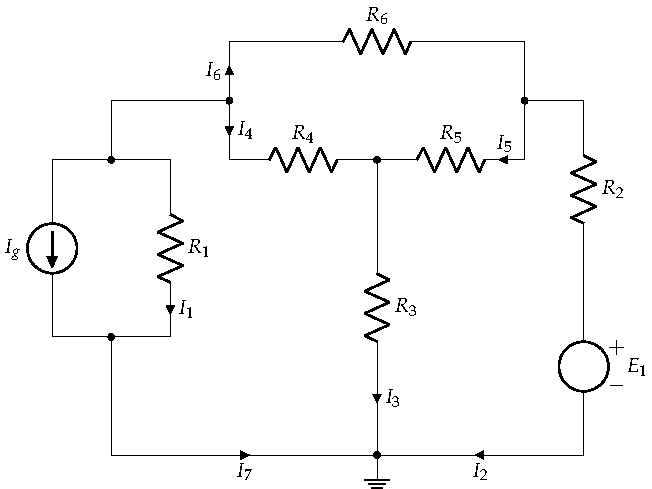
\includegraphics{figuras/BT1_12.pdf}
     \end{center}


     \subsection*{Solución}

     \underline{Resolución mediante mallas}

    \vspace{2mm}
     Se hace la transformación de la fuente de corriente en una fuente
     de tensión:
     \begin{equation*}
       \epsilon_{Ig}=I_g\cdot R_9=2\cdot 9=\qty{18}{\volt}
     \end{equation*}
     Así, el circuito está formado por 3 mallas como se muestra en la
     figura:
     \begin{center}
       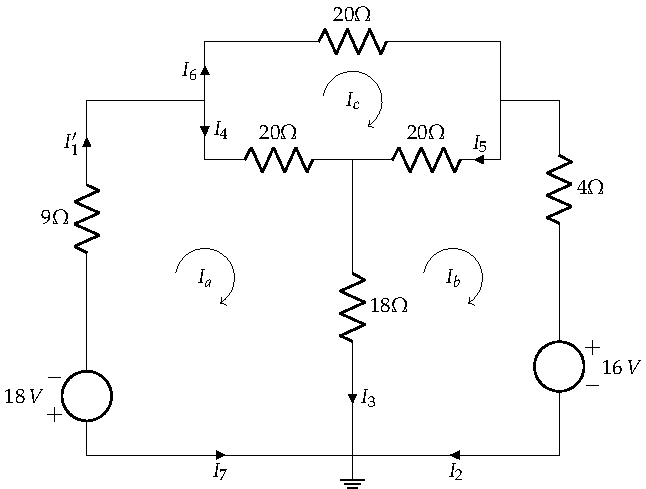
\includegraphics{figuras/BT1_12_mallas.pdf}
     \end{center}
     
     Se plantea el sistema en forma matricial:
     \begin{equation*}
       \begin{bmatrix}
         47 & -18 & -20\\
         -18 & 42 & -20\\
         -20 & -20 & 60
       \end{bmatrix}
       \cdot
       \begin{bmatrix}
         I_a\\
         I_b\\
         I_c
       \end{bmatrix}
       =
       \begin{bmatrix}
         -18\\
         -16\\
         0
       \end{bmatrix}
     \end{equation*}
     cuya solución es:
     \begin{align*}
       I_a&=\qty{-1.26}{\ampere}\\
       I_b&=\qty{-1.33}{\ampere}\\
       I_c&=\qty{-0.87}{\ampere}\\
     \end{align*}
     Estableciendo las relaciones con las corrientes de rama
     indicadas:
     \begin{align*}
       I_1'&=I_a=\qty{-1.26}{\ampere}\\
       I_2&=I_b=\qty{-1.33}{\ampere}\\
       I_3&=I_a-I_b=-1.26-(-1.33)=\qty{0.07}{\ampere}\\
       I_4&=I_a-I_c=-1.26-(-0.87)=\qty{-0.39}{\ampere}\\
       I_5&=I_c-I_b=-0.87-(-1.33)=\qty{0.46}{\ampere}\\
       I_6&=I_c=\qty{-0.87}{\ampere}\\
       I_7&=-I_a=\qty{1.26}{\ampere}\\
     \end{align*}
     La corriente $I_1$ del circuito original se obtiene aplicando el
     1LK:
     \begin{equation*}
       I_g+I_1=I_7\Rightarrow I_1=I_7-I_g=1.26-2=\qty{-0.74}{\ampere}
     \end{equation*}

     \underline{Resolución mediante nudos}

    \vspace{2mm}
     Se transforma la fuente de tensión en una de corriente:
     \begin{equation*}
       I_{\epsilon,g}=\dfrac{\epsilon_g}{R_4}=\dfrac{16}{4}=\qty{4}{\ampere}
     \end{equation*}
     quedando el circuito que se muestra en la figura:
     \begin{center}
       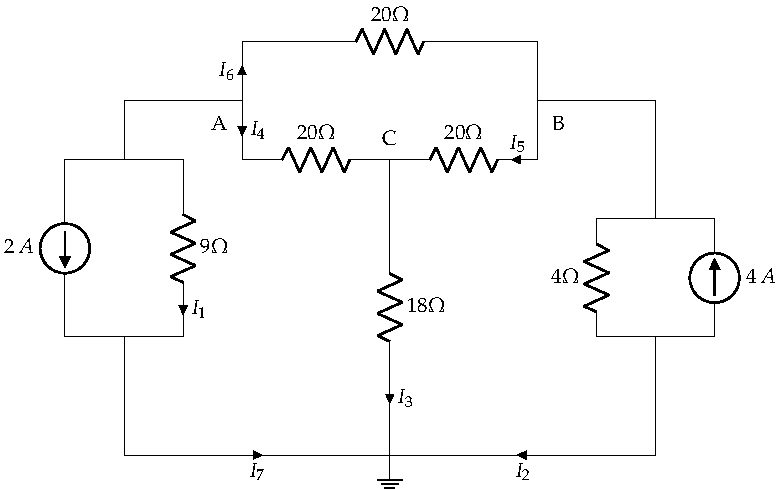
\includegraphics{figuras/BT1_12_nudos.pdf}
     \end{center}
     Con los nudos indicados, se aplica el método de nudos en su forma
     matricial:
     \begin{equation*}
       \begin{bmatrix}
         \dfrac{19}{90} & -\dfrac{1}{20} & -\dfrac{1}{20}\\[10pt]
         -\dfrac{1}{20} & \dfrac{7}{20} & -\dfrac{1}{20}\\[10pt]
         -\dfrac{1}{20} & -\dfrac{1}{20} & \dfrac{7}{45}
       \end{bmatrix}
       \cdot
       \begin{bmatrix}
         U_A\\
         U_B\\
         U_C
       \end{bmatrix}
       =
       \begin{bmatrix}
         -2\\
         4\\
         0
       \end{bmatrix}
     \end{equation*}
     cuya solución es:
     \begin{align*}
       U_A&=\qty{-6.64}{\volt}\\
       U_B&=\qty{10.66}{\volt}\\
       U_C&=\qty{1.29}{\volt}\\
     \end{align*}
     A partir de 1LK, 2LK y ley de Ohm, se obtienen las corrientes
     indicadas:
     \begin{align*}
       I_1&=\dfrac{U_A}{R_9}=\dfrac{-6.64}{9}=\qty{-0.74}{\ampere}\\[7pt]
       I_2&= I_{R_4}-I_{\epsilon,g}=\dfrac{U_B}{R_4}-4=\dfrac{10.66}{4}-4=\qty{-1.34}{\ampere}\\[7pt]
       I_3&=\dfrac{U_C}{R_{18}}=\dfrac{1.29}{18}=\qty{0.07}{\ampere}\\[7pt]
       I_4&=\dfrac{U_{AC}}{R_{20}}=\dfrac{U_A-U_C}{R_{20}}=\dfrac{-6.64-1.29}{20}=\qty{-0.39}{\ampere}\\[7pt]
       I_5&=\dfrac{U_{BC}}{R_{20}}=\dfrac{U_B-U_C}{R_{20}}=\dfrac{10.66-1.29}{20}=\qty{0.47}{\ampere}\\[7pt]
       I_6&=\dfrac{U_{AB}}{R_{20}}=\dfrac{U_A-U_B}{R_{20}}=\dfrac{-6.64-10.66}{20}=\qty{-0.87}{\ampere}\\[7pt]
       I_7&=I_g+I_1
     \end{align*}

     Se observa que los valores obtenidos son idénticos con ambos
     métodos.

    \section{Enunciado}

    Resolver el circuito por el método que se estime conveniente, obteniendo:
    \begin{itemize}
        \item El valor de las corrientes indicadas ($I_1, I_2, I_3, I_4, I_5$).
        
        \item La carga y polaridad de $C_1, C_2$ y $C_3$.

        \item La potencia entregada o absorbida por los elementos activos.
    \end{itemize}
    
    \begin{minipage}{0.65\linewidth}
      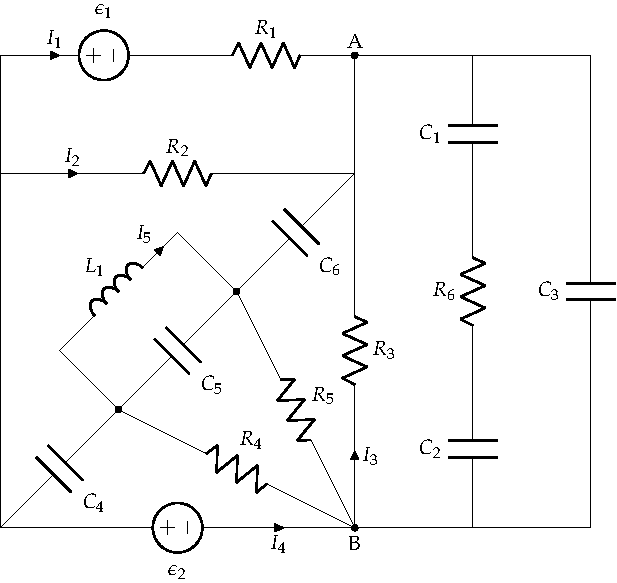
\includegraphics[scale=0.9]{figuras/BT1_ej14_enunciado.pdf}
    \end{minipage}
    \begin{minipage}{0.35\linewidth}
    
        \hspace{5mm}Datos:
    
        \vspace{2mm}    
        \hspace{5mm}$R_1 = R_2 = \qty{2}{\ohm}$
    
        \vspace{1mm}
        \hspace{5mm}$R_3 = R_4 = R_5 = R_6 = \qty{1}{\ohm}$
    
        \vspace{1mm}
        \hspace{5mm}$C_i = i\,\si{\micro\farad}$
    
        \vspace{1mm}
        \hspace{5mm}$L_1 = 1\,\si{\milli\henry}$
    
        \vspace{1mm}
        \hspace{5mm}$\epsilon_1 = \qty{10}{\volt}$
    
        \vspace{1mm}
        \hspace{5mm}$\epsilon_2 = \qty{10}{\volt}$
        
    \end{minipage}

    \subsection*{Solución}
    Para analizar el circuito, sustituimos los condensadores por circuito abierto, y la bobina por cortocircuito:

    \vspace{2mm}
    \begin{minipage}{0.3\linewidth}
      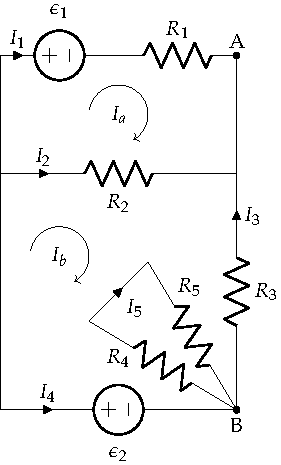
\includegraphics[scale=0.98]{figuras/BT1_ej14_mallas.pdf}
    \end{minipage}
    \hfill
    \begin{minipage}{0.65\linewidth}
    
        \vspace{-5mm}
        En el circuito resultante: $I_5=0$, $I_3=I_4$.
    
        \vspace{3mm}
        Resolviendo por mallas, definiendo las corrientes de malla $I_a$ e $I_b$ en sentido horario:
    
        %\vspace{3mm}
        \begin{minipage}{0.53\linewidth}
          \begin{equation*}
            \begin{bmatrix}
                R_1+R_2 & -R_2 \\[4pt]
                -R_2 & R_2+R_3
            \end{bmatrix} \cdot %
            \begin{bmatrix}
                I_a\\[4pt]
                I_b
            \end{bmatrix} = %
            \begin{bmatrix}
                -\epsilon_1\\[4pt]
                \epsilon_2
            \end{bmatrix}
        \end{equation*}
        \end{minipage}
        \hfill
        \begin{minipage}[c]{0.02\linewidth}
            \vspace{3mm}
            $\xrightarrow{\hspace*{0.2cm}}$ % https://latex.org/forum/viewtopic.php?t=3894
        \end{minipage}
        \hfill
        \begin{minipage}{0.4\linewidth}
            \begin{equation*}
                \begin{bmatrix}
                    4 & -2 \\[4pt]
                    -2 & 3
                \end{bmatrix} \cdot %
                \begin{bmatrix}
                    I_a\\[4pt]
                    I_b
                \end{bmatrix} = %
                \begin{bmatrix}
                    -10\\[4pt]
                    10
                \end{bmatrix}
            \end{equation*}
        \end{minipage}
    
        \vspace{3mm}
        \[
            I_a = \qty{-1.25}{\ampere} \; , \qquad I_b = \qty{2.5}{\ampere}
        \]
    
        \vspace{2mm}
        \hspace{3mm}Luego las corrientes de rama pedidas son:
    
        \vspace{-1mm}
        \[
            I_1 = I_a = \boxed{\qty{-1.25}{\ampere}} \; , \quad 
            I_2 = I_b - I_a = \boxed{\qty{3.75}{\ampere}} \; ,
        \]
        \[
            I_3 = I_4 = -I_b = \boxed{\qty{-2.5}{\ampere}} \; , \quad
                \boxed{I_5 = \qty{0}{\ampere}}
        \]
    \end{minipage}
    
    \vspace{2mm}
    
    Si no se hubiera visto inmediatamente que $I_5=0$, siempre podría haberse definido una tercera corriente de malla, $I_c=I_5$, con lo que el sistema de ecs. quedaría:
    \begin{equation*}
        \begin{bmatrix}
            R_1+R_2 & -R_2 & 0\\[4pt]
            -R_2 & R_2+R_3 & 0\\[4pt]
            0 & 0 & R_4+R_5
        \end{bmatrix} \cdot %
        \begin{bmatrix}
            I_a\\[4pt]
            I_b\\[4pt]
            I_c
        \end{bmatrix} = %
        \begin{bmatrix}
            -\epsilon_1\\[4pt]
            \epsilon_2\\[4pt]
            0
        \end{bmatrix}
    \end{equation*}
    La tercera ecuación no tiene incógnitas en común con las dos primeras, y de ella se obtiene directamente $I_c=I_5=0$.
    
    \vspace{4mm}
    Para calcular la carga en los condensadores, hay que tener en cuenta que, al no circular corriente por $R_6$ en régimen permanente del circuito, su tensión es de \qty{0}{\volt}. Luego la asociación serie de $C_1$ y $C_2$ está sometida a la tensión $U_{AB}$.
    
    \vspace{2mm}
    Asumiendo polaridad positiva en el punto A, la carga de $C_3$ es: 
    \[ 
        q_3 = C_3 \cdot U_{C_3} = C_3 \cdot (-I_3 \cdot R_3) = \boxed{\qty{7.5}{\micro\coulomb}} 
    \]
    
    \vspace{2mm}
    La carga de la asociación serie de $C_1$ y $C_2$, asumiendo polaridad positiva en A, es:
    \[ 
        q_{\textrm{serie}} = C_{12} \cdot U_{C_{12}} = C_{12} \cdot (-I_3 \cdot R_3) = \dfrac{5}{3}\,\si{\micro\coulomb} 
    \]
    
    donde la capacidad equivalente de la asociación serie ha sido calculada como: 
    \[ 
        C_{12} = \dfrac{C_1 \cdot C_2}{C_1 + C_2} = \dfrac{2}{3}\,\si{\micro\farad} 
    \]

    \vspace{-2mm}
    Al estar $C_1$ y $C_2$ asociados en serie, su carga es la misma, luego \( q_{\textrm{serie}} = \boxed{q_1 = q_2 = \dfrac{5}{3}\,\si{\micro\coulomb}} \)
    
    \vspace{3mm}
    Finalmente, la potencia entregada por los elementos activos es:
    \[ 
        P_{\epsilon1} = \epsilon_1 \cdot (-I_1) = \boxed{\qty{12.5}{\watt}}
        \qquad \qquad 
        P_{\epsilon2} = \epsilon_2 \cdot (-I_4) = \boxed{\qty{25}{\watt}} 
    \]
    

%%% Local Variables:
%%% mode: latex
%%% TeX-master: "Problemas_TC"
%%% ispell-local-dictionary: "castellano"
%%% End:



\chapter{Corriente alterna monofásica}

\section{Enunciado}
En un circuito serie RL con $R=\qty{5}{\ohm}$ y $L=\qty{0.06}{\henry}$, la tensión en bornes de la bobina es $u_L(t)=15\sin(200\,t)\,\si{\volt}$. Determinar:
\begin{itemize}
\item La tensión total.
\item Intensidad de corriente.
\item Ángulo de desfase de la intensidad respecto de la tensión.
\item Impedancia del circuito.
\end{itemize}

\subsection*{Solución}

De la expresión temporal de $u_L(t)$ se tiene que $\omega=\qty{200}{\radian\per\second}$, por lo que:
\begin{equation*}
  \overline{X}_L=\mathrm{j}\,\omega L=\mathrm{j}\,200\cdot0.06=\mathrm{j}\,\qty{12}{\ohm}
\end{equation*}
siendo la impedancia del circuito:
\begin{equation*}
  \overline{Z}_{eq}=R+\overline{X}_L= \boxed{5+\mathrm{j}\,12 = 13\phase{67.3801^\circ}\,\si{\ohm}}
\end{equation*}
(es preferible usar cuatro decimales en los ángulos, para reducir los errores numéricos por aproximación).
\vspace{2mm}

\noindent El fasor correspondiente a $u_L(t)$ es:
\begin{equation*}
  \overline{U}_L=\dfrac{15}{\sqrt{2}}\phase{0^\circ}\,\si{\volt}
\end{equation*}
Por la ley de Ohm, la intensidad de corriente en la bobina (igual a la
total, al estar en serie):
\begin{equation*}
  \overline{I}=\dfrac{\overline{U}_L}{\overline{X}_L}=\dfrac{\frac{15}{\sqrt{2}}\phase{0^\circ}}{\mathrm{j}\,12}= \boxed{0.88\phase{-90^\circ}\,\si{\ampere}}
\end{equation*}
y la tensión total, por la 2LK:
\begin{equation*}
  \overline{U}=\overline{U}_R+\overline{U}_L=5\cdot (0.88\phase{-90^\circ})+\dfrac{15}{\sqrt{2}}\phase{0^\circ}= \boxed{11.48\phase{-22.5304^\circ}\,\si{\volt}}
\end{equation*}
siendo el ángulo de desfase de la intensidad respecto a la tensión:
\begin{equation*}
  \theta_I - \theta_U = -90 - (-22.53040) =  \boxed{-67.4696^\circ}
\end{equation*}
(la ligera diferencia en los decimales respecto al ángulo de $\overline{Z}_{eq}$ es debida a las aproximaciones en decimales en operaciones previas).

%%%%%%%%%%%%%%%%%%%%%%%%%%%%%%%%%%%%%%%%%%%%%%%%%%%%%%%%%%%%%%%%%%
\section{Enunciado}

Una resistencia de \qty{5}{\ohm} y un condensador se unen en serie. La tensión en la resistencia es $u_R(t) = 25 \cdot \sin(2000t + \pi/6)\,\si{\volt}$. Si la corriente está adelantada \ang{60} respecto de la tensión aplicada, ¿cuál es el valor de la capacidad C del condensador?

\subsection*{Solución}

El ángulo de la impedancia total es:
\begin{equation*}
    \theta = \theta_V - \theta_I \quad \rightarrow \quad \theta = -\ang{60} = -\pi/3\,\si{\radian}
\end{equation*}
Y la impedancia compleja: 
\begin{equation*}
    \overline{Z} = R - \mathrm{j} \frac{1}{\omega C}
  \end{equation*}
A partir del cual puede calcularse la capacidad del condensador: 
\begin{equation*}
  \tan \theta = - \frac{1}{\omega C R} \quad \rightarrow \quad \sqrt{3} = \frac{1}{10^4 C}
\end{equation*}

\begin{equation*}
  \boxed{C = \SI[parse-numbers = false]{100\sqrt{3}/3}{\micro\farad}}
\end{equation*}

%%%%%%%%%%%%%%%%%%%%%%%%%%%%%%%%%%%%%%%%%%%%%%%%%%%%%%%%%%%%%%%%%%
\section{Enunciado}
Para determinar las constantes R y L de una bobina, se conecta en serie con una resistencia de \qty{25}{\ohm} y al conjunto se le aplica una fuente de tensión de \qty{120}{\volt} a \qty{60}{\hertz}. Se miden las tensiones en bornes de la resistencia y de la bobina, obteniendo los valores $U_R = \qty{70.8}{\volt}$ y $U_B = \qty{86}{\volt}$. ¿Cuáles son las constantes de la bobina en cuestión?

\subsection*{Solución}

Por la 2LK, se debe cumplir que:
\begin{equation*}
  \overline{U} = \overline{U}_B + \overline{U}_R
\end{equation*}


La tensión en la resistencia de \qty{25}{\ohm}, por la ley de Ohm:
\begin{equation*}
  \overline{U}_R = 25 \cdot \overline{I} \quad \rightarrow \quad I = \frac{U_R}{25} = \qty{2.83}{\ampere}
\end{equation*}
Dado que
\begin{equation*}
  \overline{Z}_B = R_B + \mathrm{j}\,\omega L_B
\end{equation*}
y conocido el módulo de la corriente que circula por el circuito, obtenemos:
\begin{equation*}
  \overline{U}_B = \overline{I} \cdot \overline{Z}_B \quad \rightarrow \quad 86 = 2.83 \, Z_B \quad \rightarrow \quad Z_B = \qty{30.37}{\ohm}
\end{equation*}
La impedancia equivalente total del circuito es:
\begin{equation*}
  \overline{Z} = (25 + R_B) + \mathrm{j}\,\omega L_B
\end{equation*}
y por la ley de Ohm:
\begin{equation*}
  \overline{U} = \overline{I} \cdot \overline{Z} \quad \rightarrow \quad 120 = 2.83 \, Z \quad \rightarrow \quad Z = \qty{42.37}{\ohm}
\end{equation*}
Planteamos el sistema de ecuaciones resultantes:
\begin{align*}
  30.37 &= \sqrt{R^2_B + (\omega L_B)^2}\\
  42.37 &= \sqrt{(25 + R_B)^2 + (\omega L_B)^2}
\end{align*}
cuyas soluciones son:
\begin{align*}
  \Aboxed{R &= \qty{5}{\ohm}}\\
  \Aboxed{L &= \qty{79.5}{\milli\henry}}
\end{align*}

%%%%%%%%%%%%%%%%%%%%%%%%%%%%%%%%%%%%%%%%%%%%%%%%%%%%%%%%%%%%%%%%%%

\section{Enunciado}
Un circuito serie RLC con $R = \qty{5}{\ohm}$ , $L = \qty{0.02}{\henry}$ y $C=\qty{80}{\micro\farad}$, tiene aplicada una tensión senoidal de frecuencia variable. Determinar los valores de la pulsación $\omega$ para los cuales la corriente:
\begin{enumerate}
\item Adelanta \qty{45}{\degree} a la tensión.
\item Está en fase con ella.
\item Retrasa \qty{45}{\degree}.
\end{enumerate}

\subsection*{Solución}
La impedancia equivalente del sistema es:

\begin{equation*}
  \overline{Z} = R + \mathrm{j}\, \left(\omega L - \frac{1}{\omega C}\right)
\end{equation*}

La tangente del ángulo es:
\begin{equation*}
  \tan \theta = \frac{\omega L - 1/\omega C}{R} = \frac{0.02\,\omega^2 - 12.5\cdot 10^3}{5\,\omega}
\end{equation*}

En esta ecuación, planteamos las condiciones particulares del enunciado:

\begin{enumerate}
\item Adelanta \qty{45}{\degree} a la tensión:
  \begin{equation*}
    \theta = -\pi/4 \quad \rightarrow \quad \tan \theta = -1
  \end{equation*}

  \begin{equation*}
    \frac{0.02\,\omega^2 - 12.5\cdot 10^3}{5\,\omega} = -1
  \end{equation*}

  \begin{equation*}
    \omega^2 + 250\,\omega - 62.5\cdot 10^4 = 0 \quad \rightarrow \quad \boxed{\omega = \qty{675.4}{\radian\per\second}}
  \end{equation*}
  (se descarta la solución negativa de la ecuación de $2^\circ$ grado por carecer de sentido físico)

\vspace{3mm}
  
\item Está en fase con ella:
  \begin{equation*}
    \theta = 0 \quad \rightarrow \quad \tan \theta = 0
  \end{equation*}

  \begin{equation*}
    0.02\,\omega = \frac{12.5\cdot 10^3}{\omega}
  \end{equation*}

  \begin{equation*}
    \boxed{\omega = \qty{790.6}{\radian\per\second}}
  \end{equation*}
  
\item Retrasa \qty{45}{\degree}:
  \begin{equation*}
    \theta = +\pi/4 \quad \rightarrow \quad \tan \theta = +1
  \end{equation*}

  \begin{equation*}
    \frac{0.02\,\omega^2 - 12.5\cdot 10^3}{5\omega} = 1
  \end{equation*}

  \begin{equation*}
    \omega^2 - 250\,\omega - 62.5\cdot 10^4 = 0 \quad \rightarrow \quad \boxed{\omega = \qty{925.4}{\radian\per\second}}
  \end{equation*}

\end{enumerate}


%%%%%%%%%%%%%%%%%%%%%%%%%%%%%%%%%%%%%%%%%%%%%%%%%%%%%%%%%%%%%%%%%%

\section{Enunciado}

Determinar el triángulo de potencias de un circuito al que se le
aplica una tensión $u(t)=340 \cdot \cos(\omega t - \pi/3)$ V y
por el que circula una intensidad de corriente
$i(t)= 13.3 \cdot \cos(\omega t-0.85)\,\si{\ampere}$.

\subsection*{Solución}

Los fasores de dicha tensión y corriente son:
\begin{align*}
  \overline{U} &= 170 \sqrt{2}\phase{\ang{-60}}\,\si{\volt}\\
  \overline{I} &= 6.65\sqrt{2}\phase{\ang{-48.7}}\,\si{\ampere}
\end{align*}

Por definición, la potencia aparente es:
\begin{equation*}
  \overline{S} = \overline{U}\cdot\overline{I}^* = 2261\phase{\ang{-11.3}}\,\si{\voltampere}
\end{equation*}

que expresada en forma binómica, resulta en los valores de $P$ y $Q$:
\begin{align*}
  P &= S \cos \theta = \qty{2217.17}{\watt}\\
  Q &= S \sin \theta = \qty{-443.03}{\var}
\end{align*}

%%%%%%%%%%%%%%%%%%%%%%%%%%%%%%%%%%%%%%%%%%%%%%%%%%%%%%%%%%%%%%%%%%

\section{Enunciado}

En el esquema de la figura, los elementos tienen los siguientes valores:
\begin{align*}
  R_1 &= R_2 = R_3 = \qty{10}{\ohm}\\
  X_1 &= X_2 = \qty{1}{\ohm}\\
  R_L &= X_L = \qty{1}{\ohm}
\end{align*}

Sabiendo que $U_{CD} = \qty{200}{\volt}$, se debe calcular:
    \begin{itemize}
    \item Intensidades de corriente $I$, $I_1$, $I_2$ e $I_3$ {en forma
        fasorial}, tomando $U_{CD}$ como referencia de fase
    \item Lectura de los vatímetros $W_1$ y $W_2$
    \end{itemize}
    
\begin{center}
  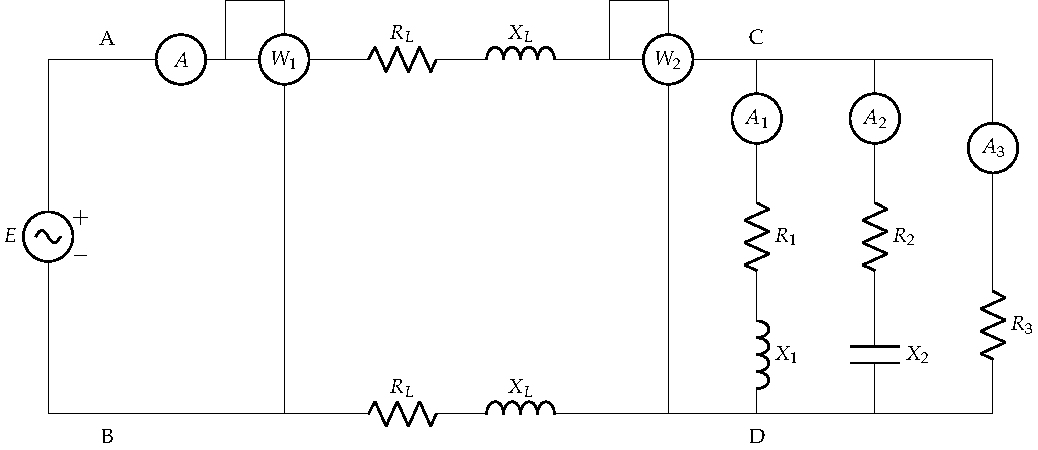
\includegraphics[width=0.85\linewidth]{figuras/BT2_08.pdf}
\end{center}

 

\subsection*{Solución}

Se dice que se tome como referencia de fase el fasor
$\overline{U}_{CD}$:

  \begin{equation*}
    \overline{U}_{CD} = 200\phase{\ang{0}}\,\si{\volt}
  \end{equation*}

  
  Esta tensión está aplicada en tres ramas en paralelo, por lo que podemos calcular las corrientes en esas ramas. En primer lugar, calculamos las impedancias:

\begin{align*}
\overline{Z}_1 &= \qty[parse-numbers=false]{10 + \mathrm{j}}{\ohm}\\
%
\overline{Z}_2 &= \qty[parse-numbers=false]{10 - \mathrm{j}}{\ohm}
\end{align*}

A continuación calculamos las corrientes de rama y la corriente total:
\begin{align*}
\overline{I}_1 &= \frac{\overline{U}_{CD}}{\overline{Z}_1} = \qty[parse-numbers=false]{19.8 - 1.98\mathrm{j}}{\ampere}\\
%
\overline{I}_2 &= \frac{\overline{U}_{CD}}{\overline{Z}_2} = \qty[parse-numbers=false]{19.8 + 1.98\mathrm{j}}{\ampere}\\
%
\overline{I}_3 &= \frac{\overline{U}_{CD}}{R_3} = 20\phase{\ang{0}}\,\si{\ampere}\\
%
\overline{I} &= \overline{I}_1 + \overline{I}_2 + \overline{I}_3 =  59.6\phase{\ang{0}}\,\si{\ampere}\\
\end{align*}

Para obtener la lectura del vatímetro 2, podemos calcular con tensión y corriente:
  \begin{align*}
\overline{S}_2 &= \overline{U}_{CD} \cdot \overline{I}^* = 11920\phase{\ang{0}}\,\si{\voltampere}\\
%
W_2 &= \mathrm{Re}\{\overline{S}_2\} = \qty{11920}{\watt}
\end{align*}

O mediante el teorema de Boucherot:
\begin{align*}
  P_1 = I_1^2 \cdot R_1 &= \qty{3959.6}{\watt}\\
  P_2 = I_2^2 \cdot R_2 &= \qty{3959.6}{\watt}\\
  P_3 = I_3^2 \cdot R_3 &= \qty{4000}{\watt}\\
  W_2 = P = P_1 + P_2 + P_3 &= \qty{11919.2}{\watt}
\end{align*}

Para el vatímetro 1, hay que tener en cuenta la potencia disipada en la línea, y aplicar nuevamente el teorema de Boucherot:
\begin{align*}
P_l &= 2 \cdot I^2 \cdot R_L = \qty{7104.3}{\watt}\\
W_1 &= W_2 + P_l = \qty{19024.3}{\watt}
\end{align*}


%%%%%%%%%%%%%%%%%%%%%%%%%%%%%%%%%%%%%%%%%%%%%%%%%%%%%%%%%%%%%%%%%%

\section{Enunciado}
En el circuito de la figura, los amperímetros $A_1$ y $A_2$ marcan $\qty{4.5}{\ampere}$ y $\qty{6}{\ampere}$, respectivamente, el voltímetro, $\qty{150}{\volt}$, y el
vatímetro, $\qty{900}{\watt}$.

Sabiendo que la frecuencia del generador es de $\qty{250}{\hertz}$ y el f.d.p. de la impedancia $Z$ es de $0.8$ en retraso, calcula:

\begin{itemize}
\item Valores de R, C y Z en forma compleja.
\item La tensión del generador.
\item Triángulo de potencias totales.
\end{itemize}

\begin{center}
  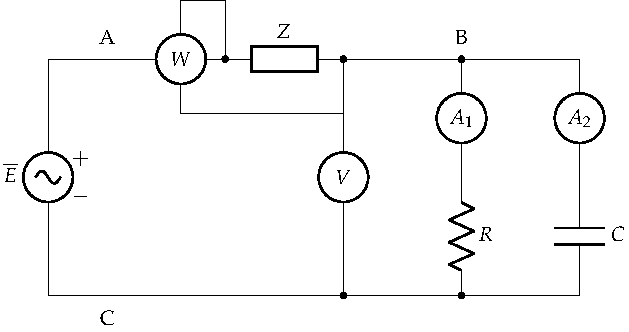
\includegraphics[width=0.6\linewidth]{figuras/BT2_09.pdf}
\end{center}


\subsection*{Solución}
\begin{enumerate}
\item Valores de R, C y Z en forma compleja.
  
\begin{equation*}
    R = \frac{U_{BC}}{A_1} = \frac{150}{4.5} = \qty{33.3}{\ohm}
  \end{equation*}
  \begin{equation*}
    X_c = \frac{U_{BC}}{A_2} = \frac{150}{6} = \qty{25}{\ohm}
  \end{equation*}
  \begin{equation*}
    C = \frac{1}{X_c\omega} = \frac{1}{25 \cdot 2 \pi \cdot 250} = \qty{25.46}{\micro\farad}
  \end{equation*}

  Tomando $\overline{U}_{BC}$ como origen de fases, $\overline{U}_{BC} = \qty[parse-numbers=false]{150\phase{0}}{\volt}$, obtenemos:
  \begin{align*}
    \overline{I}_1 &= \qty[parse-numbers=false]{4.5\phase{0}}{\ampere}\\
    \overline{I}_2 &= \qty[parse-numbers=false]{6\phase{\pi/2}}{\ampere}
  \end{align*}

  Por tanto,
  \[
    \overline{I} = \overline{I}_1 + \overline{I}_2 = \qty[parse-numbers=false]{4.5+6j}{\ampere} = 7.5\phase{\ang{53.13}}\;\si{\ampere}
  \]
  
  El vatímetro está midiendo $P_Z = U_Z \cdot I \cdot \cos \theta_Z$, y por tanto:
  \[
    U_Z = \frac{900}{7.5 \cdot 0.8} = \qty{150}{\volt}
  \]
  \[
    Z = \frac{U_Z}{I} = \qty{20}{\ohm}
  \]

    También puede obtenerse este resultado calculando primero la parte resistiva de la impedancia:
  \[
    R_Z = \frac{P_Z}{I^2} = \qty{16}{\ohm}
  \]
  y a continuación el módulo, teniendo en cuenta que $R = Z \cdot \cos \theta$:
  \[
    Z = \frac{R}{\cos \theta} = \frac{16}{0.8} = \qty{20}{\ohm}
  \]

  Con su factor de potencia obtenemos el ángulo (teniendo en cuenta que es inductiva al ser en retraso), $\theta_Z = \arccos(0.8) = \ang{36.87}$:
  \[
    \overline{Z} = 16 + 12j  = 20\phase{\ang{36.87}}\;\si{\ohm}
  \]

  
\item Tensión del generador.

  \[
    \overline{U}_{AC} = \overline{U}_{AB} + \overline{U}_{BC}
  \]
  \[
    \overline{U}_{AB} = \overline{Z} \cdot \overline{I} = 150\phase{\ang{90}}\;\si{\volt}
  \]
  \[
    \overline{U}_{AC} = 150 + 150j = 150\sqrt{2}\phase{\ang{45}}\;\si{\volt}
  \]

\item Triángulo de potencias totales en forma compleja.

  Podemos calcular a partir de la tensión y la corriente:
  \begin{align*}
    \overline{S}_T &= \overline{U}_{AC} \overline{I}^* =\\
                   &= 150\sqrt{2}\phase{\ang{45}} \cdot 7.5\phase{\ang{-53.13}} =\\
                   &= 1591\phase{\ang{-8.13}}\;\si{\voltampere}=\\
                   &= \qty[parse-numbers=false]{1575 - j225}{\voltampere}
  \end{align*}
  
  o mediante el teorema de Boucherot:
  \begin{align*}
    P_Z &= \qty{900}{\watt}\\
    P_R = 4.5^2 \cdot 33.3 &= \qty{675}{\watt}\\
    P = P_Z + P_R &= \qty{1575}{\watt}
  \end{align*}

    \vspace{-4mm}
  \begin{align*}
    Q_Z = 7.5^2 \cdot 12 &= \qty{675}{\var}\\
    Q_c = - 6^2 \cdot 25 &= \qty{-900}{\var}\\
    Q = Q_Z + Q_c &= \qty{-225}{\var}
  \end{align*}
  
  Por tanto:
  \[
    \overline{S} = P + jQ = \qty[parse-numbers=false]{1575 - j225}{\voltampere}
  \]
  
\end{enumerate}

%%%%%%%%%%%%%%%%%%%%%%%%%%%%%%%%%%%%%%%%%%%%%%%%%%%%%%%%%%%%%%%%%%

\section{Enunciado}

En el circuito de la figura, determinar las lecturas de los aparatos de medida y el balance de potencias activas y reactivas, así como el triángulo global de potencias.\\
Datos: $\; e(t)=100\sqrt{2}\cos(\omega\,t)\,\si{\volt}$;\; $R_1=2\,\Omega$;\;
$R_2=4\,\Omega$;\; $\omega L_1=3\,\Omega$;\; $\omega L_2=4\,\Omega$.

\begin{center}
  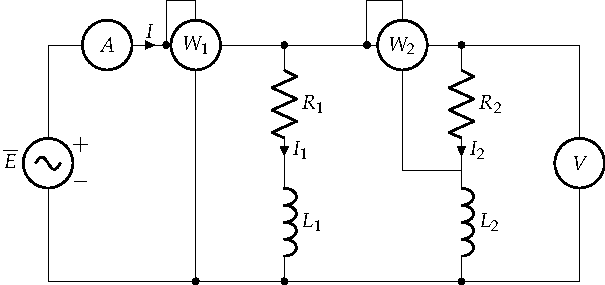
\includegraphics{figuras/BT2_11.pdf}
\end{center}

\subsection*{Solución}

El voltímetro $V$ mide la tensión eficaz de la fuente, por lo que:
\begin{equation*}
  V=\qty{100}{\volt}
\end{equation*}

Las impedancias de las dos ramas son:
\begin{align*}
  \overline{Z}_1 &= R_1 + jX_1 = \qty[parse-numbers=false]{2 + j3}{\ohm}\\
  \overline{Z}_2 &= R_2 + jX_2 = \qty[parse-numbers=false]{4 + j4}{\ohm}
\end{align*}

Calculamos el valor eficaz de las corrientes de rama:
\begin{align*}
  I_1 &= \frac{E}{Z_1} = \qty{27.74}{\ampere}\\
  I_2 &= \frac{E}{Z_2} = \qty{17.68}{\ampere}\\
\end{align*}

El vatímetro $W_2$ mide la potencia de $R_2$:
\begin{equation*}
  W_2=R_2 \cdot I_2^2= \qty{1250.33}{\watt}
\end{equation*}

El vatímetro $W_1$ mide la potencia total del circuito:
\begin{equation*}
  W_1= P_{R2} + P_{R1} = R_2 \cdot I_2^2 + R_1 \cdot I_1^2 = \qty{2789.35}{\watt}
\end{equation*}

Por otra parte, las potencias reactivas de las bobinas son:
\begin{align*}
  Q_{L1} &= X_1 \cdot I_1^2 = \qty{2308.52}{\var}\\
  Q_{L2} &= X_2 \cdot I_2^2 = \qty{1250.33}{\var}
\end{align*}

Por tanto, la potencia reactiva total es $Q = \qty{3558.82}{\var}$. Con el valor de la potencia activa podemos obtener la potencia aparente total:
\begin{equation*}
  S = \sqrt{P^2 + Q^2} = \qty{4521.69}{\voltampere}
\end{equation*}

Y, finalmente, la corriente medida por el amperímetro:
\begin{equation*}
  I = \frac{S}{V} = \qty{45.2}{\ampere}
\end{equation*}

%%%%%%%%%%%%%%%%%%%%%%%%%%%%%%%%%%%%%%%%%%%%%%%%%%%%%%%%%%%%%%%%%%

\section{Enunciado}
El circuito de la figura tiene carácter inductivo.  La impedancia de
línea es $Z=\qty[parse-numbers=false]{10\sqrt{2}}{\ohm}$ con
f.d.p. $\sqrt{2}/2$ en retraso. Tómese como referencia de fases la
intensidad total, $I$.

\vspace{3mm}
Se debe calcular:
\begin{enumerate}

\item Potencia activa y reactiva consumida por $Z$.

\item Expresiones complejas de las intensidades medidas por los
  amperímetros, $I$, $I_1$, $I_2$ e $I_3$. 

\item Expresiones complejas de las tensiones $U_{AB}$, $U_{AC}$ y
  $U_{CB}$.

\item Valores de $R_1$, $X_1$, $R_2$, $R_3$ y $X_3$.

\end{enumerate}

Datos: $\;A = \qty[parse-numbers = false]{5\sqrt{5}}{\ampere}$;\; $A_1 = \qty[parse-numbers = false]{5\sqrt{2}}{\ampere}$;\; $A_2 = \qty{5}{\ampere}$;\;  $A_3 = \qty[parse-numbers = false]{\sqrt{10}}{\ampere}$;\;  $U_{AB} = \qty{247}{\volt}$;\;  $W_1 = \qty{2350}{\watt}$;\;
$R_1 = R_3$

\begin{center}
  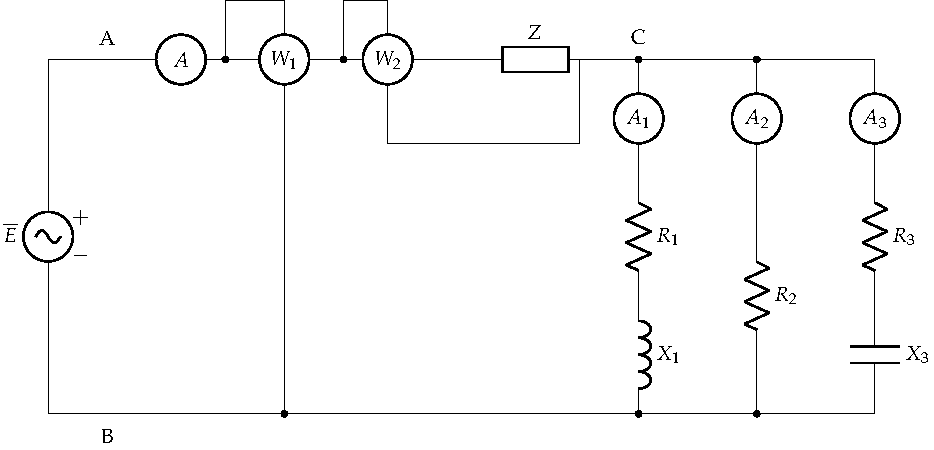
\includegraphics[width=0.8\linewidth]{figuras/BT2_17.pdf}
\end{center}


\subsection*{Solución}

Dado que disponemos de la potencia y corriente total y la tensión a
la entrada, podemos calcular el factor de potencia del circuito:
\[
\cos \phi = \frac{P_1}{U_{AB} \cdot I} = 0.851
\]

Teniendo en cuenta que la corriente total es la referencia de fases, 
\[
\overline{U}_{AB} = {247 \phase{\ang{31.68}}}\,\si{\volt}
\]

También podemos calcular la potencia reactiva del circuito
(positiva dado que el circuito es inductivo):
\[
Q = P_1 \tan \phi = \qty{1450.2}{\var}
\]


En cuanto a la impedancia $Z$, sabemos que la tensión en sus bornes
es:
\[
\overline{U}_{AC} = \overline{I} \cdot \overline{Z} =
5\sqrt{5}\phase{\ang{0}} \cdot 10\sqrt{2}\phase{\ang{45}} = {50\sqrt{10}\phase{\ang{45}}}\,\si{\volt}
\]

Se cumple que $\overline{U}_{AB} = \overline{U}_{AC} +
\overline{U}_{CB}$, y por tanto:
\[
\overline{U}_{CB} = {100\phase{\ang{10.32}}}\,\si{\volt}
\]

Por otra parte, podemos descomponer esta impedancia en:
\begin{align*}
  R &= Z \cdot \cos \phi_Z = \qty{10}{\ohm}\\
  X &= Z \cdot \sin \phi_Z = \qty{10}{\ohm}
\end{align*}

y por tanto,
\begin{align*}
P_z &= I^2 \cdot R_z = \qty{1250}{\watt}\\
Q_z &= I^2 \cdot X_z = \qty{1250}{\var}
\end{align*}

Aplicando el teorema de Boucherot, podemos calcular la potencia activa
y la potencia reactiva del circuito paralelo:
\begin{align*}
P_{CB} &= P - P_z = \qty{1100}{\watt}\\
Q_{CB} &= Q - Q_z = \qty{200.2}{\var}\\
\overline{S}_{CB} &= P_{CB} + \mathrm{j}\, Q_{CB} = {1118.07\phase{\ang{10.32}}}\,\si{\voltampere}
\end{align*}

Podemos comprobar que estos resultados son coherentes con los
resultados anteriores, usando $\overline{S}_{CB} = \overline{U}_{CB}
\cdot \overline{I}^*$.

\vspace{2mm}
Ahora podemos obtener los módulos de $R_2$, $Z_1$ y $Z_3$:
\begin{align*}
  R_2 &= \frac{U_{CB}}{I_2} = \qty{20}{\ohm}\\
  Z_1 &= \frac{U_{CB}}{I_1} = \qty[parse-numbers=false]{10\sqrt{2}}{\ohm}\\
  Z_3 &= \frac{U_{CB}}{I_3} = \qty[parse-numbers=false]{10\sqrt{10}}{\ohm}
\end{align*}

Por otra parte, la potencia activa del circuito paralelo es:
\begin{align*}
  P_{CB} &= P_1 + P_2 + P_3 =\qty{1100}{\watt}\\
  P_1 &= I_1^2 \cdot R_1 = 50 \cdot R_1\\
  P_2 &= I_2^2 \cdot R_2 = \qty{500}{\watt}\\
  P_3 &= I_3^2 \cdot R_3 = 10 \cdot R_3
\end{align*}

Dado que sabemos que $R_1 = R_3$: 
\[
   P_1 + P_3 = (50+10) \cdot R_1 = \qty{600}{\watt} \quad \rightarrow \quad R_1 = R_3 = \qty{10}{\ohm}              
\]

Con este resultado, y teniendo en cuenta el módulo de $Z_1$ y $Z_3$,
podemos calcular las respectivas reactancias:
\begin{align*}
  R_1 &= \qty{10}{\ohm}\\
  X_1 &= \sqrt{(10\sqrt2)^2 - 10^2} = \qty{10}{\ohm}\\
  \overline{Z}_1 &= 10 + 10j = {10\sqrt{2}\phase{\ang{45}}}\,\si{\ohm}
\end{align*}
\begin{align*}
  R_3 &= \qty{10}{\ohm}\\
  X_3 &= \sqrt{(10\sqrt{10})^2 - 10^2} = \qty{30}{\ohm}\\
  \overline{Z}_3 &= 10 - 30j = {10\sqrt{10}\phase{\ang{-71.56}}}\,\si{\ohm}
\end{align*}

Podemos comprobar que estas soluciones concuerdan con la potencia
reactiva de cada impedancia y con la total del circuito paralelo:
\begin{align*}
  Q_1 &= I_1^2 \cdot X_1 = \qty{500}{\var}\\
  Q_3 &= - I_3^2 \cdot X_3 = \qty{-300}{\var}\\
  Q_{CB} &= Q_1 + Q_3 =\qty{200}{\var}
\end{align*}

Con estos resultados, recordando que  $\overline{U}_{CB} =
100\phase{\ang{10.32}}$ podemos calcular las corrientes de rama en forma
compleja:
\begin{align*}
  \overline{I}_1 &=  {5\sqrt{2}\phase{\ang{-34.68}}}\,\si{\ampere}\\
  \overline{I}_2 &=  {5\phase{\ang{10.32}}}\,\si{\ampere}\\
  \overline{I}_3 &=
  {\sqrt{10}\phase{\ang{81.89}}}\,\si{\ampere}
\end{align*}

Para terminar, podemos comprobar que $\overline{I} = \overline{I}_1
+ \overline{I}_2 + \overline{I}_3$.

%%%%%%%%%%%%%%%%%%%%%%%%%%%%%%%%%%%%%%%%%%%%%%%%%%%%%%%%%%%%%%%%%%

\section{Enunciado}

La potencia reactiva del circuito de la figura es $\qty{80}{\var}$ de tipo capacitivo. La tensión en la impedancia Z está en fase con la intensidad $I_1$ y las lecturas de los aparatos son $A = \qty{4}{\ampere}$, $V = \qty{50}{\volt}$, $W = \qty{200}{\watt}$. Sabiendo que $R_1 = \qty{10}{\ohm}$ y $X_2 = \qty{50}{\ohm}$, calcula:

\begin{enumerate}
\item Las corrientes $I_1$, $I_2$, $I_3$ en forma fasorial.
\item Las reactancias $X_1$, $X_3$, y la impedancia $\overline{Z}$.
\item La fuerza electromotriz $\overline{\epsilon}$.
\end{enumerate}
\begin{center}
  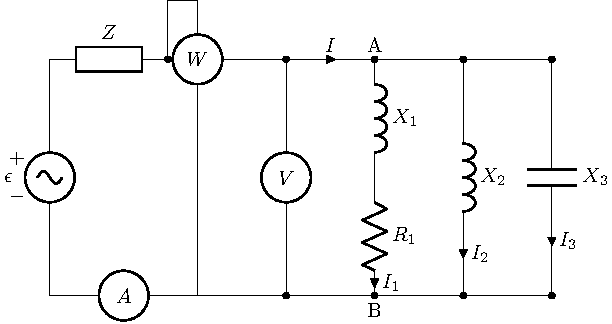
\includegraphics{figuras/BT2_circuitoCapacitivo}
\end{center}

\subsection*{Solución}


El vatímetro está midiendo la potencia activa del circuito paralelo conectado entre A y B. El único elemento que consume potencia activa en ese circuito es la resistencia $R_1$. Por tanto,

\[
  P_{R1} = 200 = I_1^2 R_1 \rightarrow I_1 = \qty[parse-numbers=false]{2\sqrt{5}}{\ampere}
\]

Dado que conocemos la tensión entre A y B, podemos determinar la impedancia de la rama 1:

\[
  Z_1 = \frac{V_{AB}}{I_1} = \qty[parse-numbers=false]{5\sqrt{5}}{\ohm}
\]
y, por tanto, obtenemos $X_1$:

\[
  Z_1 = \sqrt{R_1^2 + X_1^2} \rightarrow X_1 = \qty{5}{\ohm}
\]

\[
  \overline{Z}_1 = 10 + j5 = 5\sqrt{5}\phase{\ang{26.56}} \,\si{\ohm} 
\]

Para obtener las corrientes en forma fasorial necesitamos una referencia de fases, y será la tensión $U_{AB}$:

\[
  \overline{U}_{AB} = 50\phase{\ang{0}}\,\si{\volt}
\]

Además, del circuito AB conocemos la tensión, la corriente y la potencia, luego podemos obtener su factor de potencia:

\[
  \cos\theta_{AB} = \frac{P_{AB}}{I \cdot U_{AB}} = 1
\]

Por tanto,

\[
  \overline{I} = 4\phase{\ang{0}} \,\si{\ampere}
\]


Con $\overline{U}_{AB}$ podemos calcular el ángulo de la corriente $I_1$:

\[
  \overline{I}_1 = \frac{\overline{U}_{AB}}{\overline{Z}_1} = 2\sqrt{5}\phase{\ang{-26.56}} \,\si{\ampere} 
\]

De la misma forma podemos calcular la corriente $I_2$:
\[
  \overline{I}_2 = \frac{\overline{U}_{AB}}{jX_2} = 1\phase{\ang{-90}} \,\si{\ampere} 
\]
  
Mediante la LKC podemos obtener la corriente en la rama 3:

\[
  \overline{I} = \overline{I}_1 + \overline{I}_2 + \overline{I}_3 \rightarrow \overline{I}_3 = \qty[parse-numbers=false]{3\phase{\pi/2}}{\ampere}
\]

Aplicamos el teorema de Boucherot para obtener la reactancia de la rama 3, teniendo que en cuenta que $\cos(\theta_{AB}) = 1 \rightarrow Q_{AB} = 0$:

\begin{align*}
  Q &= Q_1 + Q_2 + Q_3 = 0\\
  Q_1 &= I_1^2 X_1 = \qty{100}{\var}\\
  Q_2 &= I_2^2 X_2 = \qty{50}{\var}\\
  Q_3 &= - I_3^2 X_3
\end{align*}

Por tanto,

\[
   Q_3 = -\qty{150}{\var} \rightarrow X_3 = \qty[parse-numbers=false]{\frac{50}{3}}{\ohm}
\]

Una forma alternativa de calcular $X_3$ es simplemente a partir del cociente entre tensión y corriente: 
\[
    \overline{Z}_3 = \frac{\overline{U}_{AB}}{\overline{I}_3} = j X_3
\]

Para determinar $\overline{Z}$ tenemos en cuenta que la potencia reactiva total es $\qty{80}{\var}$ de tipo capacitivo y que $Q_{AB} = \qty{0}{\var}$:

\[
  Q = Q_Z + Q_{AB} \rightarrow Q_Z = -\qty{80}{\var} 
\]

Por tanto:

\[
  X_Z = \frac{|Q_Z|}{I^2} = \qty{5}{\ohm}
\]

Por otra parte, el enunciado indica que la tensión en esta impedancia está en fase con la intensidad $I_1$. Por tanto, $\theta_{VZ} = \ang{-26.56}$, y $\theta_Z = \theta_{VZ} - \theta_{I} = \ang{-25.56}$. Con este ángulo podemos calcular el valor de la resistencia:

\[
  R_Z = \frac{X_Z}{|\tan\theta_Z|} = \qty{10}{\ohm}
\]

\[
  \overline{Z} =  \qty[parse-numbers=false]{10 - j5}{\ohm}
\]

Finalmente, para calcular la fuerza electromotriz podemos hacerlo de dos formas, mediante potencias o mediante tensiones:

Mediante el teorema de Boucherot calculamos la potencia activa:
\[
P = P_Z + P_{AB} = I^2 R_Z + 200 = \qty{360}{\watt}
\]
Y con la potencia reactiva $Q$ obtenemos la potencia aparente:

\[
  \overline{S} = P + jQ = \qty[parse-numbers=false]{360 -j80}{\voltampere}
\]
y la tensión:

\[
  \overline{\epsilon} = \frac{\overline{S}}{\overline{I}^*} = 90 - j20 = 10\sqrt{85}\phase{\ang{-12.53}} \,\si{\volt}
\]

Podemos llegar a este mismo resultado con un balance de tensiones:

\[
  \overline{\epsilon} = \overline{U}_Z + \overline{U}_{AB} = \overline{Z} \cdot \overline{I} + \overline{V}_{AB}
\]
%%%%%%%%%%%%%%%%%%%%%%%%%%%%%%%%%%%%%%%%%%%%%%%%%%%%%%%%%%%%%%%%%%
\section{Enunciado}
Un motor monofásico de $S = \qty{10}{\kilo\voltampere}$ y $fdp = 0.8$ está alimentado por una fuente de $\qty{230}{\volt}$ a $f = \qty{50}{\hertz}$. 
Calcula:
\begin{enumerate}
\item El valor eficaz de la corriente absorbida por el motor.
\item La potencia aparente del generador.
\item La capacidad del condensador necesario para compensar el factor de potencia a la unidad.
\item El valor eficaz de la corriente absorbida por el conjunto condensador-motor. 
\item La potencia aparente del generador necesario una vez conectado el condensador del tercer apartado.
\item Compara de forma razonada los resultados de los apartados 4 y 5 con los valores calculados en los apartados 1 y 2.
\end{enumerate}
\begin{enumerate}

\subsection*{Solución}

\item El valor eficaz de la corriente absorbida por el motor.


  \begin{align*}
  \overline{S}_m &= \overline{U} \cdot \overline{I}^*\\
%
  I &= \frac{\num{10000}}{230} = \qty{43.5}{\ampere}
\end{align*}

\item La potencia aparente del generador.
Suponemos línea ideal (sin pérdidas):
\[
  S_g = S_m = \qty{10}{\kilo\voltampere} 
\]

\item La capacidad del condensador necesario para compensar el factor de potencia a la unidad.
\begin{align*}
Q_m &= S \cdot \sin(\theta_m) = \qty{6}{\kilo\var}\\
Q_c &= Q_m\\
C &= \frac{Q_m}{\omega \cdot V^2} = \qty{361}{\micro\farad}
\end{align*}

\item El valor eficaz de la corriente absorbida por el conjunto condensador-motor. 
\begin{align*}
Q' &= \qty{0}{\var}\\
S' &= P_m = \qty{8}{\kilo\voltampere}\\
I' &= \frac{S'}{V} = \qty{34.8}{\ampere}
\end{align*}

\item La potencia aparente del generador necesario una vez conectado el condensador del tercer apartado.
\begin{align*}
S'_g &= S' = \qty{8}{\kilo\voltampere}\\
\end{align*}

\item Compara de forma razonada los resultados de los apartados 4 y 5 con los valores calculados en los apartados 1 y 2.

  La compensación de reactiva mediante la inserción del condensador ha reducido la corriente que circula por la línea y la potencia del generador en un 20\%.

\end{enumerate}

%%%%%%%%%%%%%%%%%%%%%%%%%%%%%%%%%%%%%%%%%%%%%%%%%%%%%%%%%%%%%%%%%% 

\section{Enunciado}
                                              
Un generador de corriente alterna monofásica ($f=\qty{50}{\hertz}$) alimenta a dos cargas a través de una línea de cobre. Esta línea, de resistividad $\rho=\qty{21}{\milli\ohm\milli\meter\squared\per\meter}$, tiene una longitud de $\qty{100}{\meter}$ y una sección de $\qty{16}{\milli\meter\squared}$. Las dos cargas, cuya tensión de alimentación es de $\qty{230}{\volt}$, son dos motores, uno con potencia de $\qty{7}{\kilo\watt}$ y f.d.p. de $0.65$, y otro con una potencia de $\qty{5}{\kilo\watt}$ y f.d.p. de $0.85$. Con esta información, se pide calcular:
\begin{itemize}
    \item Triángulo de potencias de cada carga y del conjunto de ambas.
    \item Valor eficaz de las corrientes en cada carga y de la corriente   total.
    \item Triángulo de potencias del generador.
    \item Valor eficaz de la tensión en bornes del generador.
    \item Capacidad del condensador a instalar en bornes de las cargas para mejorar el factor de potencia a $0.95$.
    \item Valor eficaz de la corriente entregada por el generador una vez instalado el condensador.
    \item Triángulo de potencias del generador una vez instalado el condensador.
\end{itemize}

\subsection*{Solución}

Las potencias del motor 1 son:
\begin{align*}
  P_1&=\qty{7000}{\watt}\\ 
  Q_1&=P_1\,\tan(\phi_1)=7000\cdot
                    \tan(\arccos(0.65))=\qty{8183.91}{\var}\\
  S_1&=\dfrac{P_1}{\cos(\phi_1)}=\dfrac{7000}{0.65}=\qty{10769.23}{\voltampere}
\end{align*}

y las del motor 2:
\begin{align*}
  P_2&=\qty{5000}{\watt}\\ 
  Q_2&=P_2\,\tan(\phi_2)=5000\cdot
                    \tan(\arccos(0.85))=\qty{3098.72}{\var}\\
  S_2&=\dfrac{P_2}{\cos(\phi_2)}=\dfrac{5000}{0.85}=\qty{5882.53}{\voltampere}
\end{align*}

Por el teorema de Boucherot, la potencia total de las cargas es:
\begin{align*}
  P_T&=P_1+P_2 = \qty{12000}{\watt}\\
  Q_T&=Q_1+Q_2 = \qty{11282.63}{\var}\\
  S_T&=\sqrt{P_T^2+Q_T^2}=\qty{16471.12}{\voltampere}
\end{align*}

por lo que la instalación conjunta tiene un f.d.p. de:
\begin{equation*}
  \mbox{f.d.p.}_{total}=\dfrac{P_T}{S_T}=\dfrac{12000}{16471.12}=0.7285
\end{equation*}

Usando la definición de potencia activa, se obtienen los valores eficaces de las corrientes:
\begin{align*}
  I_1&=\dfrac{P_1}{U\,\cos(\phi_1)}=\dfrac{7000}{230\cdot
       0.65}=\qty{46.82}{\ampere}\\
  I_2&=\dfrac{P_2}{U\,\cos(\phi_2)}=\dfrac{5000}{230\cdot
       0.85}=\qty{25.58}{\ampere}\\
  I_T&=\dfrac{P_T}{U\,\cos(\phi_T)}=\dfrac{12000}{230\cdot
       0.7285}=\qty{71.62}{\ampere}
\end{align*}

La resistencia de cada conductor de la línea es:
\begin{equation*}
  R_l=\rho\,\dfrac{l}{S}=21\cdot 10^{-3}\cdot
  \dfrac{100}{16}=\qty{0.13}{\ohm}
\end{equation*}

Así, las pérdidas en la línea son:
\begin{equation*}
  P_l= 2 \cdot R_l \cdot I^2=\qty{1346.2}{\watt}
\end{equation*}

y el triángulo de potencias del generador, por el teorema de Boucherot:
\begin{align*}
  P_g&=P_l+P_T= \qty{13346.23}{\watt}\\ Q_g&=Q_T=\qty{11282.63}{\var}\\
  S_g&=\sqrt{P_g^2+Q_g^2}=\qty{17476.26}{\voltampere}
\end{align*} 
por lo que la tensión a la salida del generador es:
\begin{equation*}
  U_g=\dfrac{S_g}{I}=\qty{244.4}{\volt}
\end{equation*}

Para mejorar el factor de potencia, se sabe que la potencia reactiva inicial es $\qty{11282.63}{\var}$. Puesto que se quiere un f.d.p.' de $0.95$, la potencia reactiva final será:
\begin{equation*}
  Q_T'=P_T\,\tan(\phi')=12000\cdot \tan(\arccos(0.95))=\qty{3944.21}{\var}
\end{equation*} 
siendo la potencia reactiva restante la generada por la batería de condensadores ($Q_C=Q_T'-Q_T=3944.21-11282.63=\qty{-7338.42}{\var}$). Por tanto, la capacidad del condensador equivalente a instalar es:
\begin{equation*}
  Q_c=X_c\,I^2=\dfrac{U^2}{X_c} \quad \Rightarrow \quad
  C=\dfrac{Q}{\omega\,U^2}=\dfrac{7338.42}{2\cdot\pi\cdot 50\cdot
    230^2}=\qty{441.57}{\micro\farad}
\end{equation*} 
A este mismo resultado se llegaría a partir de la expresión:
\begin{equation*}
  C=\frac{P_T \left[\tan (\phi) - \tan (\phi')\right]}{\omega
    U^2}=\dfrac{12000\left[\tan (\arccos(0.7285)) - \tan
      (\arccos(0.95))\right]}{2\cdot\pi\cdot 50\cdot 230^2}=\qty{441.66}{\micro\farad}
\end{equation*}

Una vez instalado el condensador, la potencia aparente es:
\begin{equation*}
  S_T'=\sqrt{P_T^2+Q_T'^2}=\sqrt{12000^2+3944.21^2}=\qty{12631.58}{\voltampere}
\end{equation*} 
siendo la corriente total en las cargas (entregada por el generador):
\begin{equation*}
  I'=\dfrac{S'}{U}=\dfrac{12631.58}{230}=\qty{54.92}{\ampere}
\end{equation*} 
Con esta corriente, las pérdidas en la línea se reducen a:
\begin{equation*}
  P_l'=2 \cdot R_l \cdot I'^2= \qty{791.76}{\watt}
\end{equation*} 
y el triángulo de potencias del generador, por el teorema de Boucherot:
\begin{align*}
  P_g'&=P_l'+P_T=\qty{12791.75}{\watt}\\ Q_g'&=Q_T'=\qty{3944.21}{\var}\\
  S_g'&=\sqrt{P_g'^2+Q_g'^2}=\qty{13386.02}{\voltampere}
\end{align*}

%%%%%%%%%%%%%%%%%%%%%%%%%%%%%%%%%%%%%%%%%%%%%%%%%%%%%%%%%%%%%%%%%%
\section{Enunciado}
Un generador de corriente alterna monofásica ($f = \qty{50}{\hertz}$) alimenta
a dos cargas a través de una línea de cobre. Esta línea, de
resistividad $\rho = \qty{0.017}{\ohm\per\milli\meter\squared\per\meter}$, tiene una longitud de
\qty{40}{\meter} y una sección de \qty{6}{\milli\meter\squared}. Las dos cargas, cuya tensión de
alimentación es de \qty{200}{\volt}, son:
\begin{enumerate}
\item Un motor de \qty{7}{\kilo\watt} con f.d.p. {0,7}.
\item Un grupo de lámparas fluorescentes con potencia total \qty{200}{\watt} y
  f.d.p. {0,5}.
\end{enumerate}
Se pide:
\begin{itemize}
\item Esquema del circuito señalando adecuadamente los elementos,
  corrientes y tensiones
\item Potencias activa, reactiva y aparente de cada carga
\item Valor eficaz de las corrientes en cada carga, y de la corriente
  total
\item Potencia activa y reactiva entregada por el generador
\item Valor eficaz de la tensión en bornes del generador
\item Capacidad necesaria a instalar en bornes de las cargas para
  mejorar el factor de potencia de las mismas a la unidad
\item Valor eficaz de la tensión en bornes del generador, y potencia
  aparente entregada por el mismo una vez instalada la capacidad
  determinada en el apartado anterior
\end{itemize}

\subsection*{Solución}

\begin{enumerate}
  
\item El esquema del circuito es el mostrado en la figura.

\begin{center}
  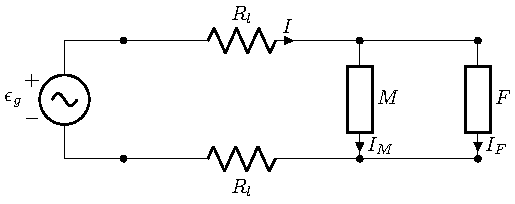
\includegraphics{figuras/circuito_cargas.pdf}
\end{center}
  
\item Potencias activa, reactiva y aparente de cada carga.

\begin{align*}
  P_M &= \qty{7000}{\watt}\\
  Q_M &= \qty{7141.4}{\var}\\
  S_M &= \qty{10000}{VA}\\
  P_F &= \qty{200}{\watt}\\
  Q_F &= \qty{346.4}{\var}\\
  S_F &= \qty{400}{VA}
\end{align*}

\item Valor eficaz de las corrientes en cada carga, y de la corriente
  total.

  \begin{align*}
    I_M &= S_M / V = \qty{50}{\ampere}\\
    I_F &= S_F / V = \qty{2}{\ampere}
  \end{align*}

  Por teorema de Boucherot la potencia total en cargas es:

\begin{align*}
  P_T &= \qty{7200}{\watt}\\
  Q_T &= \qty{7487.8}{\var}\\
  S_T &= \qty{10387.9}{VA}
\end{align*}

Y, por tanto, la corriente total es:
\[
  I = S_T / U = \qty{51.9}{\ampere}
\]

\item Potencia activa y reactiva entregada por el generador.
La resistencia de la línea (una resistencia por cada conductor) es:

\[
R_L = \rho L/S = \qty{0.113}{\ohm}
\]

La potencia activa disipada en la línea es:

\[
P_L = 2 \cdot I^2 R_L = \qty{611.48}{\watt}
\]

Por tanto, la potencia entregada por el generador es:

\begin{align*}
P_g &= P_L + P_T = \qty{7811.5}{\watt}\\
Q_g &= Q_T = \qty{7487.8}{\var}\\
S_g &= \qty{10820.7}{VA}
\end{align*}

\item Valor eficaz de la tensión en bornes del generador.
\[
U_g = S_g / I = \qty{208.3}{\volt}
\]

\item Capacidad necesaria a instalar en bornes de las cargas para
  mejorar el factor de potencia de las mismas a la unidad.

  \[
C = \frac{Q_t}{\omega V^2} = \qty{595.9}{\micro\farad}
\]


\item Valor eficaz de la tensión en bornes del generador, y potencia
  aparente entregada por el mismo una vez instalada la capacidad
  determinada en el apartado anterior.

  Una vez instalado este condensador, la corriente total en las cargas es:

\[
I' = P_T / V = \qty{36}{\ampere}
\]

La potencia disipada en la línea es ahora:

\[
P'_L = 2 \cdot I'^2 R_L = \qty{293.8}{\watt} 
\]

Y la potencia entregada por el generador es:
\begin{align*}
P'_g &= \qty{7493.8}{\watt}\\
Q'_g &= \qty{0}{\var}\\
S'_g &= \qty{7493.8}{VA}
\end{align*}

Por tanto, la tensión en bornes del generador es:

\[
U'_g = S'_g / I' = \qty{208.2}{\volt}
\]

\end{enumerate}
%%%%%%%%%%%%%%%%%%%%%%%%%%%%%%%%%%%%%%%%%%%%%%%%%%%%%%%%%%%%%%%%%% 

\section{Enunciado}


Un generador de corriente alterna ($f = \SI{50}{\hertz}$) alimenta una instalación eléctrica a través de una línea de cobre ($\rho = \SI{0.017}{\ohm\milli\meter\squared\per\meter}$) de $\SI{25}{\milli\meter\squared}$ de sección. La instalación eléctrica está compuesta por un motor de $S_m = \SI{10}{\kilo\voltampere}$ y $\mathrm{fdp} = 0.8$, una instalación de alumbrado fluorescente de $P_f = \SI{800}{\watt}$ y $\mathrm{fdp} = 0.9$, y diversas cargas electrónicas con una potencia conjunta $P_e = \SI{540}{\watt}$ y $\mathrm{fdp} = 0.5$ en retraso.

Suponiendo que las cargas trabajan a su tensión nominal de $\SI{230}{\volt}$ y que están situadas a $\SI{100}{\meter}$ del generador, calcule:

\begin{enumerate}
\item Triángulo de potencias total de las cargas ($P_T$, $Q_T$, $S_T$) y factor de potencia.
\item Valor eficaz de la corriente que circula por la línea.
\item Potencia disipada en la línea.
\item Triángulo de potencias del generador ($P_g$, $Q_g$, $S_g$) y factor de potencia.
\item Valor eficaz de la tensión de salida del generador.
\item Capacidad del banco de condensadores a instalar en bornes de la carga necesario para reducir la corriente que circula por la línea a un valor de $\SI{45}{\ampere}$.
\end{enumerate}

Independientemente del resultado obtenido, suponga que la capacidad instalada es $C = \SI{172}{\micro\farad}$. En estas condiciones, calcule:
\begin{enumerate}[resume]
\item Potencia aparente de las cargas (incluyendo al banco de condensadores)
\item Valor eficaz de la corriente que circula por la línea y potencia disipada en la misma.
\item Triángulo de potencias del generador y factor de potencia.
\item Tensión de trabajo del generador.
\end{enumerate}

\subsection*{Solución}

\begin{enumerate}
\item Triángulo de potencias total de las cargas ($P_T$, $Q_T$, $S_T$) y factor de potencia.

    Motor:
  \begin{align*}
    P_m &= \SI{8000}{\watt}\\
    Q_m &= \SI{6000}{\var}\\
  \end{align*}

  Alumbrado
  \begin{align*}
    P_f &= \SI{800}{\watt}\\
    Q_f &= \SI{387.5}{\var}\\
  \end{align*}

  Cargas Electrónicas
  \begin{align*}
    P_e &= \SI{540}{\watt}\\
    Q_e &= \SI{935.3}{\var}\\
  \end{align*}

  Total (Teorema de Boucherot)
  \begin{align*}
    P_T &= P_m + P_f + P_e = \SI{9340}{\watt}\\
    Q_T &= Q_m + Q_f + Q_e = \SI{7322.8}{\var}\\
  \end{align*}

  Por tanto, $S_T = \SI{11868.4}{\voltampere}$ y
  $\mathrm{fdp}_T = 0.787$.

\item Valor eficaz de la corriente que circula por la línea.
\[
  I = \frac{S_T}{U} = \frac{11868.4}{230} = \SI{51.6}{\ampere}
\]

\item Potencia disipada en la línea.

  \begin{align*}
  R &= \SI{0.068}{\ohm}\\
  P_L &= 2 \cdot I^2 \cdot R = \SI{362.1}{\watt}
  \end{align*}

\item Triángulo de potencias del generador ($P_g$, $Q_g$, $S_g$) y factor de potencia.


  \begin{align*}
    P_g &= P_T + P_L = \SI{9702.1}{\watt}\\
    Q_g &= Q_T = \SI{7322.8}{\var}\\
    S_g &= \SI{12155.4}{\voltampere}\\    
    \mathrm{fdp} &= 0.798
  \end{align*}

\item Valor eficaz de la tensión de salida del generador.

  \[
    U_g = \frac{S_g}{I} = \SI{235.6}{\volt}
  \]

\item Capacidad del banco de condensadores a instalar en bornes de la carga necesario para reducir la corriente que circula por la línea a un valor de $\SI{45}{\ampere}$.

  Si la corriente en línea se reduce a $\SI{45}{\ampere}$ la potencia aparente resultante en cargas (incluyendo al condensador) es $S'_T = 230 \cdot 45 = \SI{10350}{\voltampere}$. Por tanto, $Q'_T = \SI{4459.5}{\var}$. Así, es necesario instalar un banco de condensadores que aporte $Q_c = Q_T - Q'_T = \SI{2863.3}{\var}$.

\[
C = \frac{Q_c}{\omega U^2} = \SI{172.3}{\micro\farad}
\]

  
\end{enumerate}

Independientemente del resultado obtenido, suponga que la capacidad instalada es $C = \SI{172}{\micro\farad}$. En estas condiciones, calcule:
\begin{enumerate}[resume]
\item Potencia aparente de las cargas (incluyendo al banco de condensadores)
\[
S'_T = \sqrt{P^2_T + Q'^2_T} = \SI{10350.1}{\voltampere}
\]

\item Valor eficaz de la corriente que circula por la línea y potencia disipada en la misma.
\[
I' = \frac{S'_T}{U} = \SI{45}{\ampere}
\]

\[
  P'_L = 2 \cdot I'^2 \cdot R = \SI{275.4}{\watt}
\]

\item Triángulo de potencias del generador y factor de potencia.
  \begin{align*}
    P'_g &= P_T + P'_L = \SI{9615.4}{\watt}\\
    Q'_g &= Q'_T = \SI{4459.5}{\var}\\
    S'_g &= \SI{10599.2}{\voltampere}\\    
  \end{align*}

\item Tensión de trabajo del generador.
\[
U'_g = \frac{S'_g}{I'} = \SI{235.5}{\volt}
\]
\end{enumerate}

%%%%%%%%%%%%%%%%%%%%%%%%%%%%%%%%%%%%%%%%%%%%%%%%%%%%%%%%%%%%%%%%%% 
\section{Enunciado}

Calcular la corriente $i(t)$ del circuito de la figura.

\begin{center}
  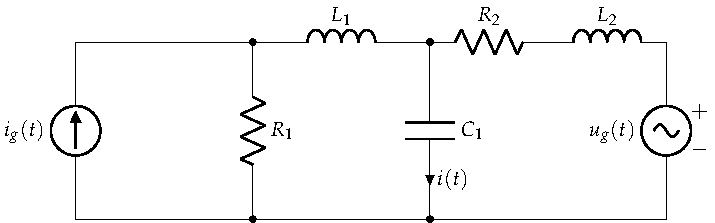
\includegraphics{figuras/BT2_13.pdf}
\end{center}
Datos: $i_g(t) = 10\sqrt{2}\sin(100t)\unit{\ampere}$; $R_1 = R_2 = \qty{1}{\ohm}$; $L_1 = L_2 = \qty{0.01}{\henry}$; $C_1 = \qty{0.01}{\farad}$; $u_g(t) = 10\sqrt{2}\cos(100t)\unit{\volt}$
\subsection*{Solución}

En primer lugar, se deben indicar las dos expresiones de tensión y
corriente en una misma función senoidal. En este caso, se opta por
pasar la corriente a función coseno:
\begin{align*}
  u(t)=\sqrt{2}\,10\,\cos(100\,t) \;\si{\volt}  &\quad\Rightarrow\quad \overline{U}=10\phase{\ang{0}} V\\
  i_g(t)=\sqrt{2}\,10\,\cos(100\,t-\frac{\pi}{2}) \;\si{\ampere} &\quad\Rightarrow\quad \overline{I}_g=10\phase{\ang{-90}} A
\end{align*}
Se transforma la fuente de corriente en una fuente de tensión en serie
con la resistencia $R_1$:
\begin{equation*}
  \overline{U}_{I_g}=\overline{I}_g \cdot R_{1}=(10\phase{\ang{-90}})\cdot 1=10\phase{\ang{-90}} V
\end{equation*}
y estableciendo corrientes de malla como se muestra en la siguiente
figura, se puede plantear el sistema de ecuaciones en forma matricial
tras determinar el valor de las impedancias:
\begin{align*}
  \overline{X}_L&=\mathrm{j}\,\omega\,L=\mathrm{j}\, 100\cdot 0.01= \mathrm{j}\,\Omega\\
  \overline{X}_C&=-\mathrm{j}\,\dfrac{1}{\omega\,C}=-\mathrm{j}\, \dfrac{1}{100\cdot 0.01}= -\mathrm{j}\,\Omega
\end{align*}

\begin{center}
  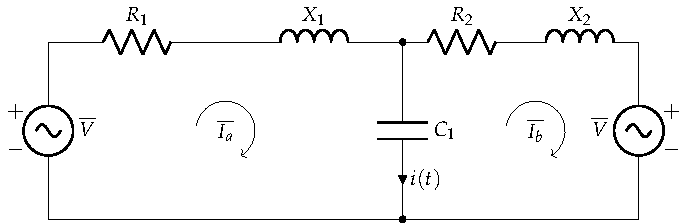
\includegraphics{figuras/BT2_13_mod.pdf}
\end{center}

\begin{equation*}
  \begin{bmatrix}
    1+\mathrm{j}-\mathrm{j} & -(-\mathrm{j})\\
    -(-\mathrm{j}) & 1+\mathrm{j}-\mathrm{j}
  \end{bmatrix}
  \cdot
  \begin{bmatrix}
    \overline{I_a}\\
    \overline{I_b}
  \end{bmatrix}
  =
  \begin{bmatrix}
    10\phase{-90^\circ}\\
    -10\phase{0^\circ}
  \end{bmatrix}
\end{equation*}
cuya solución es:
\begin{align*}
  \overline{I}_a&=0\;\si{\ampere}\\
  \overline{I}_b&=-10\;\si{\ampere}
\end{align*}
Dado que la corriente $i(t)$ se relaciona con las corrientes de malla
por:
\begin{equation*}
  \overline{I}=\overline{I}_a-\overline{I}_b=0-(-10)=10\;\si{\ampere}
\end{equation*}
siendo su expresión temporal:
\begin{equation*}
  i(t)=\sqrt{2}\,10\,\cos(100\,t)\;\si{\ampere}
\end{equation*}

%%%%%%%%%%%%%%%%%%%%%%%%%%%%%%%%%%%%%%%%%%%%%%%%%%%%%%%%%%%%%%%%%%


%%% Local Variables:
%%% mode: latex
%%% TeX-master: "Problemas_TC"
%%% ispell-local-dictionary: "castellano"
%%% End:



\chapter{Corriente alterna trifásica}
\section{Enunciado}
 
El receptor trifásico de la figura tiene secuencia de fases inversa y tensión de línea 200$\sqrt{3}$ V. Su potencia activa es 12 kW, y el vatímetro 2 ($W_2$) indica 6 kW. Hallar:
\begin{itemize}
    \item Valor de la impedancia $\overline{Z}$, en forma compleja.
    \item Fasores correspondientes a las intensidades de línea.
\end{itemize}

\begin{center}
  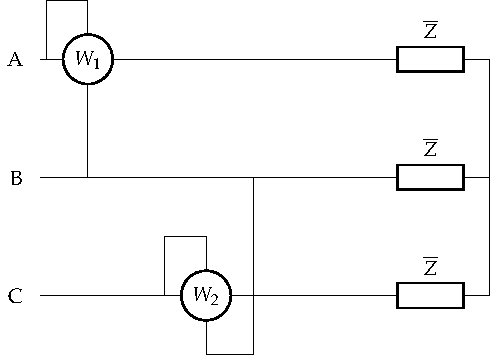
\includegraphics[width=0.5\linewidth]{figuras/ej6_BT3.pdf}
\end{center}

\subsection*{Solución}

El receptor está conectado en estrella a tres hilos (sin neutro). Al ser secuencia de fases inversa, se tiene que al principio de la línea:
\begin{align*}
    &\overline{U}_{AB}=200\sqrt{3}\phase{-120^\circ}\;\text{V} \\
    &\overline{U}_{BC}=200\sqrt{3}\phase{0^\circ}\;\text{V} \\
    &\overline{U}_{CA}=200\sqrt{3}\phase{120^\circ}\;\text{V}  \\
    &\overline{U}A=200\phase{-90^\circ}\;\text{V}\\
    &\overline{U}_B=200\phase{30^\circ}\;\text{V}\\
    &\overline{U}_C=200\phase{150^\circ}\;\text{V}
\end{align*}

La potencia activa del receptor es 12000 W, por lo que:
\begin{equation*}
    P_T=3\cdot R_f\cdot I_f^2=3\cdot \dfrac{U_f^2}{R_f} \quad\rightarrow\quad R_f=3\cdot\dfrac{U_f^2}{P_T}=3\cdot \dfrac{200^2}{12000}=10\;\Omega\text{/fase}
\end{equation*}
Dado que se trata de un receptor equilibrado, por el método de los dos vatímetros, se cumple que:
\begin{equation*}
    P_T=W_1+W_2 \quad\rightarrow\quad W_1=P_T-W_2=12000-6000=6000\;\text{W}
\end{equation*}
Con esto se puede obtener la potencia reactiva consumida por la carga. Al tratarse de una secuencia inversa:
\begin{equation*}
    Q_T=\sqrt{3}\; (W_1-W_2)=\sqrt{3}\cdot (6000-6000)=0\;\text{var}
\end{equation*}
Por lo que la impedancia $\overline{Z}$ es puramente resistiva de valor $\overline{Z}={10\phase{0^\circ}}\Omega/\mathrm{fase}$.

\vspace{3mm}
A partir de la tensión de fase, y aplicando la ley de Ohm, se puede obtener la intensidad de fase que circula por el receptor (igual a la de línea, por estar en estrella)\footnote{Con el módulo de $I_L$, podría determinarse también el valor de $\overline{Z}$ considerando la medida de $W_2$. Según el método de los dos vatímetros, se sabe que $W_2=U_L\,I_L\,\cos(\theta+30^\circ)=200\sqrt{3}\cdot 20\cdot \cos(\theta+30^\circ)=6000\Rightarrow \theta = 0^\circ\Rightarrow\overline{Z}=10\Omega/\mathrm{fase}$}:
\begin{align*}
    \overline{I}_A&=\dfrac{\overline{U}_{A}}{\overline{Z}}=\dfrac{200\phase{-90}}{10}={20\phase{-90^\circ}\;\text{A}}\\
    \overline{I}_B&=\dfrac{\overline{U}_{B}}{\overline{Z}}=\dfrac{200\phase{30}}{10}={20\phase{30^\circ}\;\text{A}}\\
    \overline{I}_C&=\dfrac{\overline{U}_{C}}{\overline{Z}}=\dfrac{200\phase{150}}{10}={20\phase{150^\circ}\;\text{A}}
\end{align*}



%%%%%%%%%%%%%%%%%%%%%%%%%%%%%%%%%%%%%%%%%%%%%%%%%%%%%%%%%%%%%%%%%%%%%%%%%

 \section{Enunciado}
 
En el sistema trifásico de la figura, de secuencia de fases directa y $f=60$ Hz, el receptor equilibrado disipa una potencia total $P_T = \qty{51984}{\watt}$ con un factor de potencia de 0,6 en
retraso. Sabiendo que el amperímetro indica 76$\sqrt{3}$ A,
determinar:
\begin{itemize}
    \item  Lecturas de los vatímetros 1 y 2
    \item  Valor de la impedancia $\overline{Z}$ en forma compleja
    \item Capacidad mínima para mejorar el factor de potencia a 0,95
\end{itemize}

\begin{center}
  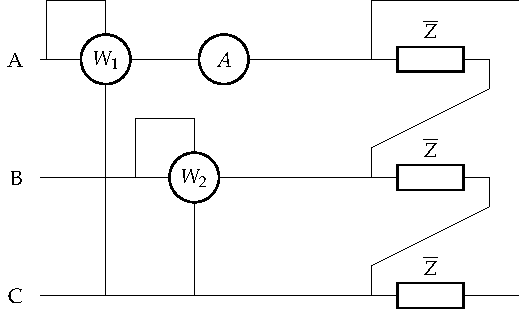
\includegraphics[width=0.53\linewidth]{figuras/ej4_BT3.pdf}
\end{center}


\subsection*{Solución}
Las tres impedancias están conectadas en triángulo. El amperímetro mide el módulo de la corriente de línea $\overline{I}_A$. Dado que se conoce el factor de potencia $\cos(\varphi)=0.6$ (en retraso), se tiene que $\varphi=+53.1301^\circ$. Por el método de los dos vatímetros:
\begin{equation*}
    P_T=W_1+W_2=51\,984=\sqrt{3}\, U_L\, I_L\, \cos{\phi}\quad\rightarrow\quad U_L=\dfrac{P_T}{\sqrt{3}\, I_L\,\cos{\phi}}=\dfrac{51\,984}{\sqrt{3}\cdot 76\sqrt{3}\cdot 0.6}=380\;\text{V}
\end{equation*}
por lo que: 
\begin{align*}
    W_1&=U_L\,I_L\,\cos(\phi-30^\circ)=380\cdot 76\sqrt{3}\cdot\cos(53.1301^\circ-30^\circ)=\qty{46000.65}{\watt}\\
    W_2&=U_L\,I_L\,\cos(\phi+30^\circ)=380\cdot 76\sqrt{3}\cdot\cos(53.1301^\circ+30^\circ)=\qty{5983.35}{\watt}
\end{align*}
  
Considerando la referencia de tensiones para SFD:
\begin{equation*}
    \overline{U}_{AB}=380\phase{120^\circ}\,\si{\volt}\qquad 
    \overline{U}_{BC}=380\phase{0^\circ}\,\si{\volt}\qquad 
    \overline{U}_{CA}=380\phase{-120^\circ}\,\si{\volt}
\end{equation*}
El módulo de las corrientes de fase es:
\begin{equation*}
    I_f=\dfrac{I_L}{\sqrt{3}}=\dfrac{76\sqrt{3}}{\sqrt{3}}=76\,\si{\ampere}
\end{equation*}
y, dado que $\phi=\theta_U-\theta_I\rightarrow \theta_I=\theta_U-\phi$, se tiene que las corrientes de fase son: 
\begin{equation*}
    \overline{I}_{AB}=76\phase{66.87^\circ}\,\si{\ampere}\qquad 
    \overline{I}_{BC}=76\phase{-53.13^\circ}\,\si{\ampere}\qquad 
    \overline{I}_{CA}=76\phase{-173.13^\circ}\,\si{\ampere}
\end{equation*}
Por tanto, el valor de la impedancia $\overline{Z}$ es: 
\begin{equation*}
    \overline{Z}=\dfrac{\overline{U}_{AB}}{\overline{I}_{AB}}=\dfrac{\overline{U}_{BC}}{\overline{I}_{BC}}=\dfrac{\overline{U}_{CA}}{\overline{I}_{CA}}=5\phase{53.1301^\circ}\,\Omega={3+\mathrm{j}\,4}\;\Omega
\end{equation*}

Al indicarse que la capacidad para mejorar el factor de potencia debe ser la {mínima}, se opta por una configuración en {triángulo} para el banco de condensadores. La potencia reactiva inicial $Q_T$ es:
\begin{equation*}
    Q_T=P\cdot \tan(\phi)=51\,984\cdot \tan(53.1301^\circ)=\qty{69312}{\var}
\end{equation*}
El nuevo factor de potencia es $\cos{\phi'}=0.95\rightarrow\phi'=18.1949^\circ$, siendo la potencia reactiva $Q_T'$:
\begin{equation*}
    Q_T'=P\cdot \tan(\phi')=51\,984\cdot \tan(18.1949^\circ)=\qty{17086.34}{\var}
\end{equation*}
Por tanto, la potencia reactiva que genera la batería de condensadores a conectar es: 
\begin{equation*}
    Q_C=Q_T'-Q_T=17\,086.34-69\,312=\qty{-52225.66}{\var}
\end{equation*}
teniendo una capacidad $C$ (conectada en triángulo, $C_{\triangle}$) de:
\begin{equation*}
    C_{\triangle}=\dfrac{|Q_C|}{3\cdot\omega\cdot U^2}=\dfrac{52\,225.66}{3\cdot 2\,\pi\, 60\cdot 380^2}= \qty{319.8}{\micro\farad}
\end{equation*}



%%%%%%%%%%%%%%%%%%%%%%%%%%%%%%%%%%%%%%%%%%%%%%%%%%%%%%%%%%%%%%%%%%%%%%%%%

\section{Enunciado}
 
En el sistema trifásico de la figura, de secuencia de fases inversa y tensión de línea 200$\sqrt{3}$ V, los dos receptores son equilibrados, con impedancias $\overline{Z}_1 = 6+\mathrm{j}\,8\;\Omega$ y $\overline{Z}_2 = 8+\mathrm{j}\,6\;\Omega$. Determinar:
\begin{itemize}
    \item  Lecturas de los amperímetros.
    \item  Lecturas de los vatímetros y la potencia compleja total.
\end{itemize}
\begin{center}
  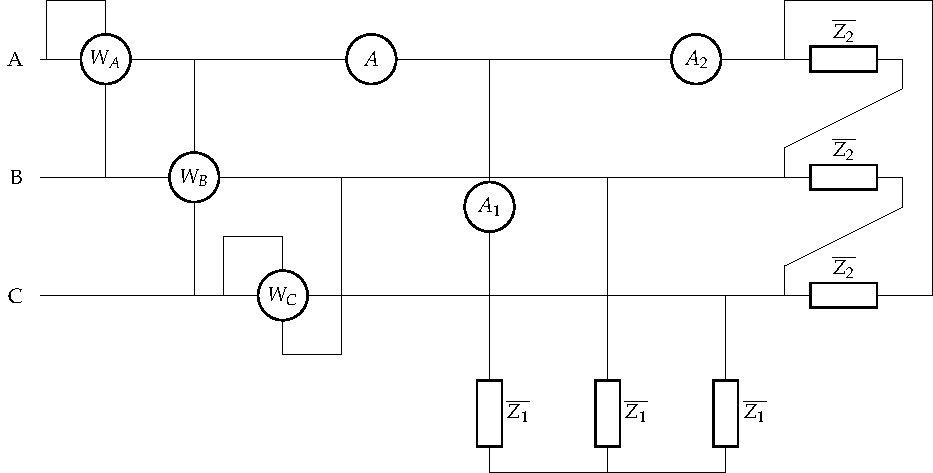
\includegraphics[width=.85\linewidth]{figuras/ej5_BT3.pdf}
\end{center}

\subsection*{Solución}
Las impedancias $\overline{Z}_1$ están conectadas en estrella, mientras que las $\overline{Z}_2$ lo están en triángulo; entre ellas, están conectadas en paralelo. 

\vspace{3mm}
El amperímetro $A_1$ mide la corriente de línea que va a la impedancia $\overline{Z}_{1,A}$ (módulo de $\overline{I}_{1,A}$). Puesto que se tiene la tensión de fase $\overline{U}_{A}$ y el valor de la impedancia de $\overline{Z}_1$, la corriente $\overline{I}_{1,A}$ es:
\begin{equation*}
    I_{1,A} = \frac{U_f}{Z_1} = \qty{20}{\ampere}
\end{equation*}
por lo que el amperímetro $A_1$ marca 20 A. 

\vspace{3mm}
El amperímetro $A_2$ mide la corriente de línea que va a la impedancia $\overline{Z}_{2,A}$ (módulo de $\overline{I}_{2,A}$). La corriente que circula por esta impedancia (corriente de fase) es:
\begin{equation*}
    I_{2f} = \frac{U}{Z_2} = \qty[parse-numbers = false]{20\sqrt{3}}{\ampere}
\end{equation*}

Por tanto, el amperímetro $A_2$, que marca el módulo de la corriente de línea $I_{2,A}$: 
\begin{equation*}
    I_{2,A}= \sqrt{3}\cdot I_{2f} = \qty{60}{\ampere}
\end{equation*}
por lo que el amperímetro $A_2$ marca 60 A.

\vspace{3mm}
El amperímetro $A$ mide la corriente de línea $I_A$. Se puede obtener su valor mediante la LKC, para lo que sería necesario obtener los fasores de las corrientes $I_{1A}$ e $I_{2A}$ o, de forma más sencilla, mediante el Teorema de Boucherot. Las potencias de cada carga y total son:

\begin{itemize}
    \item Carga $\overline{Z}_1$:
    \begin{align*}
        P_1&=3\cdot R_1\cdot I_{f,1}^2=3\cdot 6\cdot 20^2=\qty{7200}{\watt}\\
        Q_1&=3\cdot X_1\cdot I_{f,1}^2=3\cdot 8\cdot 20^2=\qty{9600}{\var}
    \end{align*}
    \item Carga $\overline{Z}_2$:
    \begin{align*}
        P_2&=3\cdot R_2\cdot I_{f,2}^2=3\cdot 8\cdot (20\sqrt{3})^2=\qty{28800}{\watt}\\
        Q_2&=3\cdot X_2\cdot I_{f,2}^2=3\cdot 6\cdot (20\sqrt{3})^2=\qty{21600}{\var}
    \end{align*}
    \item Total:
    \begin{align*}
        P_T&=P_1+P_2=7200+28\,800=\qty{36000}{\watt}\\
        Q_T&=Q_1+Q_2=9600+21\,600=\qty{31200}{\var}\\
        \overline{S}_T&=P_T+j\,Q_T={36\,000+\mathrm{j}\,31\,200 = 47\,638.64\phase{40.9144^\circ} \;\text{VA}}
    \end{align*}
\end{itemize}

Por tanto, teniendo en cuenta que $S_T = \sqrt{3} \, U \cdot I$, obtenemos la corriente de línea (lectura del amperímetro A):
\begin{equation*}
  I = \frac{47\,638.6}{\sqrt{3} \cdot 200\sqrt{3}} = \qty{79.4}{\ampere}
\end{equation*}


El vatímetro $W_A$ mide la corriente de línea $A\;(I_A)$ y la tensión de línea $U_{AB}$; el vatímetro $W_B$ mide la corriente de línea $B\;(I_B)$ y la tensión de línea $U_{AC}=-U_{CA}$; por último, el vatímetro $W_C$ mide la corriente de línea $C\;(I_C)$ y la tensión de línea $U_{BC}$.

\vspace{3mm}
Por el método de los dos vatímetros, $W_A$ y $W_C$ miden la potencia total: 
\begin{align*}
  P_T &= W_A + W_C =\qty{36000}{\watt}\\
  Q_T &= \sqrt{3}\cdot (W_A - W_C) = \qty{31200}{\var}
\end{align*}

Por tanto:
\begin{align*}
  W_A &= \qty{27007.43}{\watt}\\
  W_C &= \qty{8993.58}{\watt}
\end{align*}

Por otra parte, el vatímetro $W_B$ mide la potencia reactiva total entre $\sqrt{3}$:
\begin{equation*}
  W_B = \frac{Q_T}{\sqrt{3}}=\qty{18013.85}{\watt}
\end{equation*}


%%%%%%%%%%%%%%%%%%%%%%%%%%%%%%%%%%%%%%%%%%%%%%%%%%%%%%%%%%%%%%%%%%%%%%%%%

\section{Enunciado}
 
El sistema trifásico de la figura es de 380 V a 50 Hz y secuencia de fases inversa. $\overline{Z}$ es un elemento pasivo ideal, tal que el factor global de potencia es la unidad. El motor es de 1,8 CV, rendimiento 90\% y factor de potencia 0,8. Determinar:
\begin{itemize}
    \item  Impedancia $\overline{Z}$ en forma compleja.
    \item  Intensidad en el motor.
    \item  Fasores intensidad de línea.
    \item  Lectura de los aparatos de medida: V, A, W$_1$, W$_2$ y W$_3$.
\end{itemize}
\begin{center}
  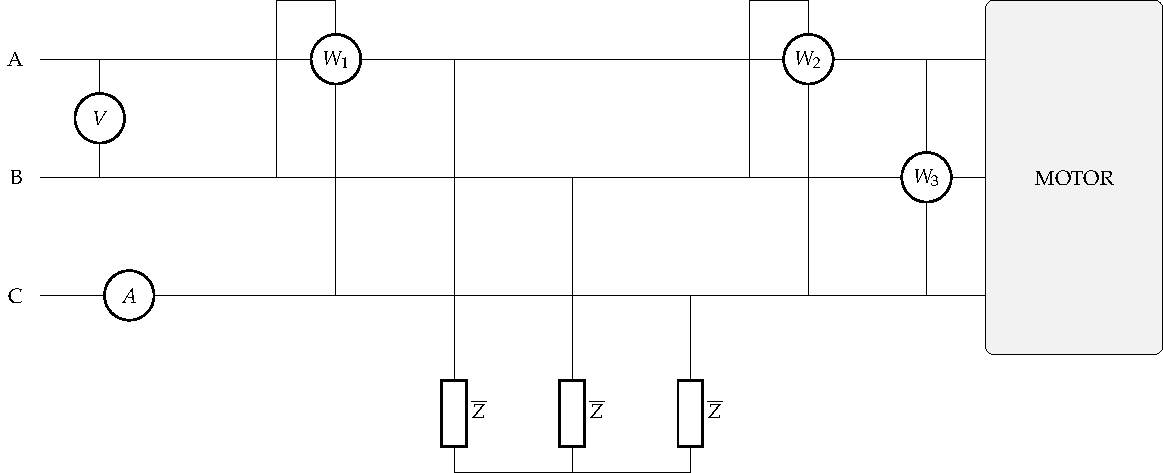
\includegraphics[width=\linewidth]{figuras/ej7_BT3.pdf}
\end{center}

\subsection*{Solución}
El motor tiene una potencia útil de 1.8 CV que, en W:
\begin{equation*}
  P_u=1.8\cdot 746=1342.8\;\text{W}    
\end{equation*}
Su potencia activa, considerando el rendimiento, es:
\begin{equation*}
  P_M=\dfrac{P_u}{\eta}=\dfrac{1342.8}{0.9}=1492\;\text{W}
\end{equation*} 


Al ser secuencia de fases inversa, se tiene que al principio de la
línea:
\begin{align*}
  &\overline{U}_{AC}=380\phase{-120^\circ}\;\text{V} \\
  &\overline{U}_{BC}=380\phase{0^\circ}\;\text{V} \\
  &\overline{U}_{CA}=380\phase{120^\circ}\;\text{V}  \\
  &\overline{U}_A=220\phase{-90^\circ}\;\text{V}\\
  &\overline{U}_B=220\phase{30^\circ}\;\text{V}\\
  &\overline{U}_C=220\phase{150^\circ}\;\text{V}
\end{align*}

Se sabe que el factor de potencia global es 1. Dado que el motor tiene
un comportamiento inductivo, con factor de potencia de $0.8$, y la
impedancia $\overline{Z}$ es un elemento pasivo ideal, {esta debe ser
  una batería de condensadores} conectados en estrella que mejoren el
factor de potencia a 1. La potencia reactiva del motor $Q_M$ es:
\begin{equation*}
  Q_M=P_M\cdot \tan(\phi_M)=1492\cdot \tan(36.8699^\circ)=1119\;\text{var}
\end{equation*}
El factor de potencia global es $\cos{\phi}=1\rightarrow\phi=0^\circ$,
siendo la potencia reactiva $Q_T$:
\begin{equation*}
  Q_T=P_M\cdot \tan(\phi)=1492\cdot \tan(0)=0\;\text{var}
\end{equation*}
Por tanto, la potencia reactiva que genera la batería de condensadores
(impedancia $\overline{Z}$) es:
\begin{equation*}
  Q_Z=Q_T-Q_M=0-1119=-1119\;\text{var}
\end{equation*}
que, al estar conectados en estrella, tienen una impedancia de:
\begin{equation*}
  Q_Z=3\cdot \dfrac{U_f^2}{Z} \quad\rightarrow\quad Z=3\cdot \dfrac{U_f^2}{Q_Z}=3\cdot \dfrac{220^2}{-1119}=-129.76\;\Omega \quad\rightarrow\quad \overline{Z}={-\mathrm{j}\,129.76}\;\Omega\text{/fase}
\end{equation*}

La intensidad en el motor es:
\begin{equation*}
  I_M=\dfrac{P_M}{\sqrt{3}\,U_L\,\cos(\phi_M)}=\dfrac{1492}{\sqrt{3}\cdot 380\cdot 0.8}= \qty{2.83}{\ampere}
\end{equation*}

Dado que los condensadores no consumen potencia activa, las
intensidades de línea se pueden calcular a partir de la potencia
activa consumida por el motor, y el factor de potencia global de la
instalación:
\begin{equation*}
  I_L=\dfrac{P_T}{\sqrt{3}\cdot U_L\cdot \cos{(\phi})}=\dfrac{1492}{\sqrt{3}\cdot 380\cdot 1}=2.27\;\text{A}
\end{equation*}
que, en forma fasorial, teniendo en cuenta que $\phi'=0^\circ$:
\begin{align*}
  \overline{I}_{A}&={2.27\phase{-90^\circ}\;\text{A}}\\
  \overline{I}_{B}&={2.27\phase{30^\circ}\;\text{A}}\\
  \overline{I}_{C}&={2.27\phase{150^\circ}\;\text{A}}
\end{align*}

El voltímetro $V$ mide el módulo de la tensión
$\overline{U}_{AB}\rightarrow V={380}$ {V}. El amperímetro $A$ mide el
módulo de la corriente $\overline{I}_C\rightarrow A={2.27}$ {A}. El
vatímetro $W_1$ mide la corriente $\overline{I}_A$ y la tensión
$\overline{U}_{BC}$, por lo que:
\begin{equation*}
  W_1=U_{BC}\cdot I_A\cdot \cos{(\theta_{{U}_{BC}}-\theta_{{I}_A})}= 380\cdot 2.27\cdot \cos(0-(-90^\circ))={0\;\text{W}}
\end{equation*}

También podemos obtener este valor teniendo en cuenta que, por la
conexión que tiene, y al tratarse de SFI, está midiendo
$-Q_T/\sqrt{3}$. Al tener la instalación en su conjunto un
$\cos(\phi)=0$, la potencia reactiva total es $Q_T=0$, por lo que
$W_1=0$ W.

\vspace{3mm}
El vatímetro $W_2$ mide la corriente $\overline{I}_{A,M}$ y la tensión
$\overline{U}_{BC}$. El ángulo de $\overline{I}_{A,M}$, considerando
que el motor está conectado en estrella, es
$\theta_{{I}_{A,M}}=\theta_{{U}_{A,M}}-\phi_M=-90^\circ-(-36.8699^\circ)=126.8699^\circ$,
por lo que:
\begin{equation*}
  W_2=U_{BC}\cdot I_{A,M}\cdot \cos{(\theta_{{U}_{BC}}-\theta_{{I}_{A,M}})}= 380\cdot 2.83\cdot \cos(0-126.8699^\circ)={-645.24\;\text{W}}
\end{equation*}
Como alternativa, viendo la conexión que tiene, y al tratarse de SFI,
se sabe que está midiendo $-Q_M/\sqrt{3}$. Al tener el motor una
$Q_M=1119$ var, $W_2=-1119/\sqrt{3}=-646.05$ W.

  \vspace{3mm}
Por último, el vatímetro $W_3$ mide el módulo de la corriente
$\overline{I}_{B,M}$ y de la tensión $\overline{U}_{AC}$. El ángulo de
$\overline{I}_{B,M}$, considerando que el motor está conectado en
estrella, es
$\theta_{I_{B,M}}=\theta_{U_{B,M}}-\phi_M=30^\circ-(-36.8699^\circ)=66.8699^\circ$;
y el ángulo de
$\overline{U}_{AC}=-\overline{U}_{CA}=380\phase{-60^\circ}$\,\si{\volt}, por lo
que:
\begin{equation*}
  W_3=U_{AC}\cdot I_{B,M}\cdot \cos{(\theta_{{U}_{AC}}-\theta_{{I}_{B,M}})}= 380\cdot 2.83\cdot \cos(-60^\circ-66.8699^\circ)={645.24\;\text{W}}
\end{equation*}

De otra forma, por la conexión que tiene, y al tratarse de SFI, se
sabe que está midiendo $Q_M/\sqrt{3}$, por lo que
$W_3=1119/\sqrt{3}=646.05$ W.


 \section{Enunciado}

 Una plantación agrícola emplea dos bombas sumergibles para extraer
 agua de un pozo y transportarla a través de un sistema de riego por
 goteo. Estas dos bombas están alimentadas a \SI{400}{\volt} por una
 línea trifásica en secuencia de fases directa y frecuencia
 $\SI{50}{\hertz}$. Una de las bombas funciona con un motor trifásico
 de $\SI{30}{\kilo\watt}$ y factor de potencia de $0.78$. La otra bomba
 trabaja con un motor de $\SI{7.5}{\kilo\watt}$ y factor de potencia
 de $0.67$.  La línea que alimenta estas dos bombas es resistiva, con
 resistividad $\rho = \SI{0.017}{\ohm\milli\meter\squared\per\meter}$,
 longitud de \SI{300}{m} y una sección de
 \SI{35}{\milli\meter\squared}.
 
 \begin{enumerate}
 \item Calcula el triángulo de potencias (potencia activa, reactiva, y
   aparente) de cada carga, y total de las cargas (a la salida de la
   línea).
 \item Calcula el valor eficaz de la corriente de línea de
   cada carga y de la corriente total.
 \item Determina la lectura de los siguientes aparatos de medida
   conectados a la entrada de las cargas:
   \begin{itemize}
   \item Un vatímetro en la fase A, midiendo tensión entre las fases A
     y C.
   \item Un vatímetro en la fase B, midiendo tensión entre las fases B
     y C.
   \item Un vatímetro en la fase C, midiendo tensión entre las fases B
     y A.
   \end{itemize}
 \item Calcula el triángulo de potencias a la entrada de la línea.
 \item Calcula el valor eficaz de la tensión a la entrada de la línea.
 \item Calcula los condensadores que se deben conectar a la salida de
   la línea para mejorar el factor de potencia del sistema hasta la
   unidad. Indica modo de conexión más eficiente.
 \end{enumerate}

Una vez conectados los condensadores del último apartado:
\begin{enumerate}[resume]
\item Calcula el valor eficaz de la corriente de línea total.
\item Calcula el triángulo de potencias a la entrada de la línea.
\item Calcule el valor eficaz de la tensión a la entrada de la línea.
\item Determina la lectura de los vatímetros descritos anteriormente.
\end{enumerate}

\vspace{3mm}

\subsection*{Solución}

\begin{minipage}{0.32\linewidth}         
    
    \vspace{-5mm}

    El esquema del circuito que nos plantean es:

    \vspace{8mm}
    (donde desconocemos si los motores de las bombas están conectados en $\wye$ o $\triangle$)    
\end{minipage}
\hfill%
\begin{minipage}{0.6\linewidth}  

    \vspace{-3mm}
    \begin{center}
        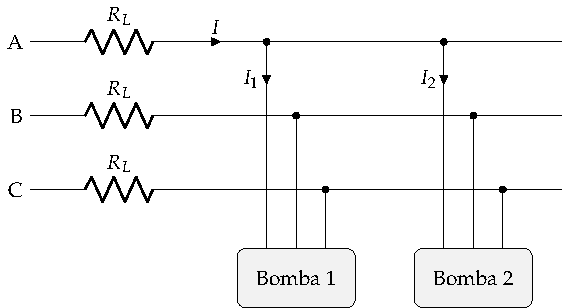
\includegraphics[width=1\textwidth]{figuras/BT3_ej5_bombas.pdf}
    \end{center}   
\end{minipage}

\vspace{4mm}
 Las potencias de cada carga son:

\vspace{-2mm}
\begin{minipage}{0.5\linewidth}         
    \begin{align*}
        P_1 &= \SI{30}{\kilo\watt}\\[4pt]
        Q_1 &= P_1\tan \theta_1 = \SI{24.06}{\kilo\voltampere}_r\\[4pt]
        S_1 &= \sqrt{P_1^2 + Q_1^2} = \SI{38.46}{\kilo\voltampere}
    \end{align*}   
\end{minipage}
\hfill%
\begin{minipage}{0.5\linewidth}  
    \begin{align*}
        P_2 &= \SI{7.5}{\kilo\watt}\\[4pt]
        Q_2 &= P_2 \tan \theta_2 = \SI{8.31}{\kilo\voltampere}_r\\[4pt]
        S_2 &= \sqrt{P_2^2 + Q_2^2} = \SI{11.19}{\kilo\voltampere}
    \end{align*} 
\end{minipage}

\vspace{5mm}
 Aplicando Boucherot, el triángulo de potencias total es:
 \begin{align*}
   P_T &= P_1 + P_2 = \SI{37.5}{\kilo\watt}\\[4pt]
   Q_T &= Q_1 + Q_2 = \SI{32.37}{\kilo\voltampere}_r\\[4pt]
   S_T &= \sqrt{P_T^2 + Q_T^2} = \SI{49.54}{\kilo\voltampere}
 \end{align*}

\vspace{2mm}
 Por tanto, el ángulo de la impedancia global es:

\[
  \tan(\theta) = \frac{Q_T}{P_T} = 0.8632 \quad \rightarrow \quad \theta =
  \ang{40.8}
\]

\vspace{2mm}
Las corrientes en cada carga son:
\begin{align*}
  I_1 &= \frac{S_1}{\sqrt{3} \,U} = \SI{55.51}{\ampere}\\
  I_2 &= \frac{S_2}{\sqrt{3} \,U} = \SI{16.15}{\ampere}
\end{align*}

La corriente total es:
\[
  I = \frac{S_T}{{\sqrt{3} \,U}} = \SI{71.5}{\ampere}
\]

\begin{center}
    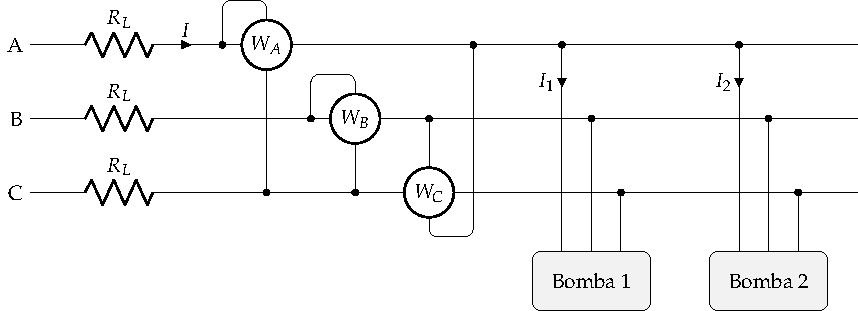
\includegraphics[width=.9\textwidth]{figuras/BT3_ej5_bombas_vatimetros.pdf}
\end{center}

\vspace{2mm}
Denominaremos $W_1$ al vatímetro conectado en la fase A midiendo
tensión entre las fases A y C, y $W_2$ al vatímetro conectado en
la fase B midiendo tensión entre las fases B y C. 

\vspace{3mm}
La conexión de estos 2 vatímetros corresponde al montaje de Aron.

\vspace{4mm}
Teniendo en cuenta que se trata de una SFD: 
\begin{align*}
  W_1 + W_2 &= P_T\\[3pt]
  W_1 - W_2 &= \frac{Q_T}{\sqrt{3}}
\end{align*}

Sumando y restando las dos expresiones anteriores se obtiene, respectivamente:
\begin{align*}
  W_1 &= \frac{1}{2} \, \left(P_T + \frac{Q_T}{\sqrt{3}} \right) = \SI{28.09}{\kilo\watt}\\[3pt]
  W_2 &= \frac{1}{2} \, \left(P_T - \frac{Q_T}{\sqrt{3}} \right) = \SI{9.41}{\kilo\watt}
\end{align*}

También podemos obtener estos resultados con las siguientes ecuaciones:
\begin{align*}
  W_1 &= U I \cos(\ang{30} - \theta) = \SI{28.09}{\kilo\watt}\\[3pt]
  W_2 &= U I \cos(\ang{30} + \theta) = \SI{9.41}{\kilo\watt}
\end{align*}

Por otra parte, el vatímetro de la fase C mide:
\[
  W_{C, BA} = - \frac{Q_T}{\sqrt{3}} = - \SI{18.66}{\kilo\watt}
\]

La resistencia de la línea (una resistencia por cada conductor) es:
\[
R_L = \rho \, \frac{l}{S} = \SI{0.146}{\ohm}
\]

La potencia activa disipada en la línea es:
\[
P_L = 3 \cdot I^2 \, R_L = \SI{2234.8}{\watt}
\]

Por tanto, la potencia a la entrada de la línea es:
\begin{align*}
    P_g &= P_L + P_T = \SI{39.73}{\kilo\watt}\\[3pt]
    Q_g &= Q_T = \SI{32.33}{\kilo\voltampere}_r\\[3pt]
    S_g &= \sqrt{P_g^2 + Q_g^2} = \SI{51.22}{\kilo\voltampere}
\end{align*}

\vspace{2mm}
Y la tensión a la salida del generador (entrada de la línea) es:
\[
U_g = \frac{S_g}{\sqrt{3} \, I} = \SI{413.64}{\volt}
\]

Para mejorar el factor de potencia a la unidad en las cargas, se necesita una batería de condensadores conectados en triángulo en las cargas (a la salida de la línea). Cada uno de los tres condensadores debe tener una capacidad de:
\[
C_{\triangle} = \frac{Q_T}{3 \, \omega \, U^2} = \SI{214.4}{\micro\farad}
\]

\begin{center}
    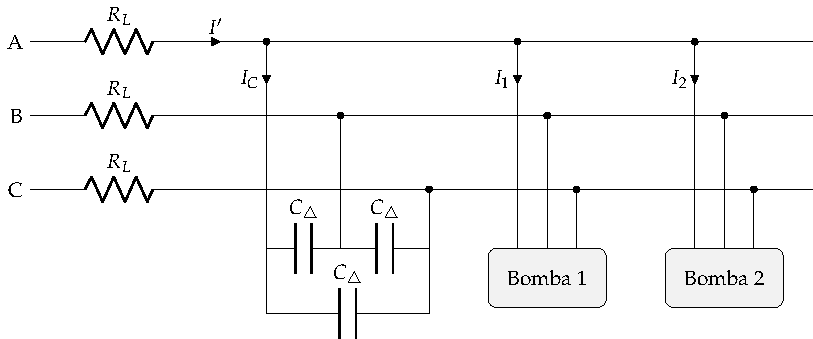
\includegraphics[width=.85\textwidth]{figuras/BT3_ej5_bombas_condensadores.pdf}
\end{center}

Una vez instalada la batería de condensadores, la corriente total a la salida de la línea es:
\[
I' = \frac{P_T}{\sqrt{3} \, U} = \SI{54.13}{\ampere}
\]

La potencia disipada en la línea es ahora:
\[
P'_L = 3 \cdot I'^2 \, R_L = \SI{1282.9}{\watt} 
\]

Por tanto, el triángulo de potencias a la entrada de la línea es:
\begin{align*}
P'_g &= P'_L + P_T = \SI{38.78}{\kilo\watt}\\[3pt]
Q'_g &= Q'_T = \SI{0}{\kilo\voltampere}_r\\[3pt]
S'_g &= \SI{38.78}{\kilo\voltampere}
\end{align*}

Consecuentemente, la tensión a la entrada de la línea es:
\[
U' = \frac{S'_g}{\sqrt{3} \, I'} = \SI{413.63}{\volt}
\]

\begin{center}
    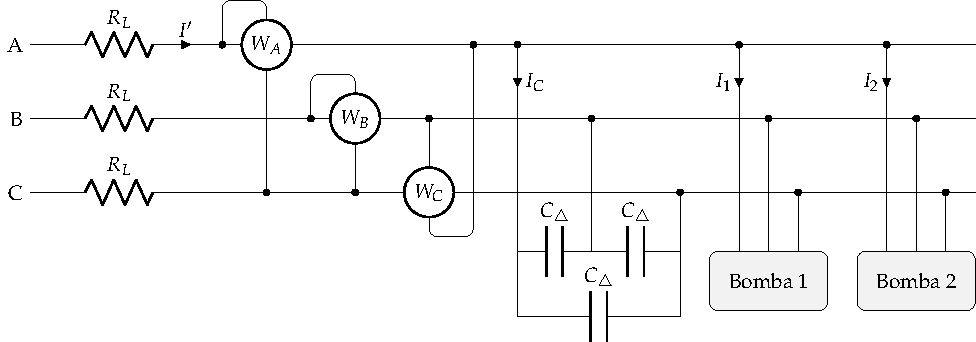
\includegraphics[width=1\textwidth]{figuras/BT3_ej5_bombas_condensadores_vat.pdf}
\end{center}

\vspace{2mm}
Con la inserción de los condensadores, los vatímetros miden:
\[
    W'_{C, BA} = - \frac{Q'_T}{\sqrt{3}} = \SI{0}{\watt}
\]

\vspace{-2mm}
Y dado que $\; W'_1 - W'_2 = \dfrac{Q'_T}{\sqrt{3}} = 0 \,$:

\vspace{2mm}
\[
    W'_1 + W'_2 = P_T 
    \qquad \rightarrow \qquad    
    W'_1 = W'_2 = \frac{1}{2} \; P_T = \SI{18.75}{\kilo\watt}
\]



\section{Enunciado}

El circuito de la figura es de secuencia de fases directa y 50 Hz. Determinar:
\begin{enumerate}
\item Potencias activas y reactivas totales.
\item Capacidad mínima de los condensadores a instalar para mejorar el factor de potencia total hasta la unidad.
\item Intensidades de línea, en forma fasorial, una vez mejorado el factor de potencia.
\end{enumerate}
\begin{minipage}{0.4\linewidth}

  \vspace{-30mm}
  Datos: 

  \begin{align*}
    \overline{Z}_1 &= {100\phase{\ang{60}}}\,\unit{\ohm}\\
      W_1 &= \SI{300}{\watt}\\
      W_2 &= \SI{300}{\watt}\\
      V &= {200\sqrt{3}}\,\unit{\volt}
  \end{align*}
\end{minipage}
\begin{minipage}{0.6\linewidth}
  \begin{center}
    \includegraphics{figuras/ZyZt}
  \end{center}
\end{minipage}

\subsection*{Solución}

Los dos vatímetros miden la potencia de la impedancia $Z_2$:
\begin{align*}
  P_2 &= W_1 + W_2 = \SI{600}{\watt}\\
  Q_2 &= \sqrt{3}\cdot (W_1 - W_2) = \SI{0}{\volt\ampere_r}
\end{align*}

Para calcular la potencia de $Z_1$, debemos obtener la corriente de fase:
\[
  I_{1f} = \frac{U}{Z_1} = {2\sqrt{3}}\,\unit{\ampere}
\]

Por tanto:
\begin{align*}
  P_1 &= 3 \cdot I_{1f}^2 \, R_1 = 3 \cdot (2\sqrt{3})^2 \cdot 100\, \cos(\ang{60}) = \SI{1800}{\watt}\\
  Q_1 &= 3 \cdot I_{1f}^2 \, X_1 = 3 \cdot (2\sqrt{3})^2 \cdot 100\, \sin(\ang{60}) = {1800\sqrt{3}}\,\unit{\volt\ampere_r}
\end{align*}

Aplicando Boucherot:
\begin{align*}
  P &= P_1 + P_2 = \SI{2400}{\watt}\\
  Q &= Q_1 + Q_2 = {1800\sqrt{3}}\,\unit{\volt\ampere_r}
\end{align*}

Para compensar completamente el factor de potencia, se deben instalar tres condensadores en triángulo con capacidad:
\[
  \qquad\qquad\qquad\quad C_\triangle = \frac{Q}{3 \, \omega \, U^2} = \SI{27.57}{\micro\farad} \qquad \text{(en cada fase)}
\]

\vspace{2mm}
Al instalar estos condensadores, la corriente que circula por la línea es:
\[
  P = \sqrt{3} \cdot U \cdot I' \quad \rightarrow \quad I' = \SI{4}{\ampere}
\]

En forma fasorial, teniendo en cuenta que $\theta' = \ang{0}$:
\begin{align*}
  \overline{I}_A &= {4\phase{\ang{90}}}\,\unit{\ampere}\\
  \overline{I}_B &= {4\phase{\ang{-30}}}\,\unit{\ampere}\\
  \overline{I}_C &= {4\phase{\ang{-150}}}\,\unit{\ampere}
\end{align*}





\section{Enunciado}

En la figura, dos vatímetros miden una carga trifásica inductiva
equilibrada, alimentada a una tensión $U = \SI{400}{\volt}$. El
vatímetro $W_B$ indica una lectura de \SI{11320}{\watt}, y el
vatímetro $W_C$ indica una lectura de \SI{1815}{\watt}. A partir de
esta información se pide:

\begin{enumerate}
\item Determinar la secuencia de fases del sistema.
\item Triángulo de potencias de la carga.
\item Impedancia equivalente de la carga en estrella y
  en triángulo.
\item Tensión de alimentación a la entrada de la línea
  $U_1$, sabiendo que la línea de alimentación es resistiva pura con
  valor $R = \SI{0.1}{\ohm}$.
\item Capacidad de los condensadores que se deben
  conectar en bornes de la carga para conseguir mejorar su factor de
  potencia a la unidad. Determinar las nuevas lecturas de los
  vatímetros $W_B$ y $W_C$.
\end{enumerate}

\begin{center}
  \includegraphics[width=0.65\linewidth]{figuras/BT3_10.pdf}
\end{center}

\subsection*{Solución}

El vatímetro $W_C$ está conectado de forma que mide la potencia
reactiva:
\[
  W_C = \mp \frac{Q}{\sqrt{3}}
\]

Dado que el vatímetro está conectado entre B y A, el signo negativo
corresponde a SFD y el positivo a SFI. Dado que la carga es inductiva, consume potencia reactiva, luego $Q > 0$. Como $W_C > 0$, debemos elegir el signo positivo, lo que
implica SFI.

\vspace{2mm}
Al vatímetro $W_B$ podríamos añadirle un hipotético vatímetro
$W_A$ conectado en la fase A, midiendo tensión entre A y C, para
emplear el método de los dos vatímetros:
\begin{align*}
W_B + W_A &= P\\
W_B - W_A &= \frac{Q}{\sqrt{3}} = W_C
\end{align*}

Sumando ambas ecuaciones obtenemos:
\[
  P = 2 \,W_B - W_C = \SI{20825}{\watt}
\]

La potencia reactiva se calcula directamente con el vatímetro $W_C$:
\[
  Q = \sqrt{3} \, W_C = \SI{3143.7}{\var}
\]

Por tanto:
\[
  \overline{S} =
  21\,060.9\phase{\ang{8.58}}\,\unit{VA}
\]

El módulo de la impedancia en triángulo se obtiene con
$Z_{\triangle} = U / I_f$. Teniendo en cuenta que $S = \sqrt{3} \,U \,I$
y que $I = \sqrt{3} \,I_f$, obtenemos $I_f = S / 3U$. Por tanto:
\[
  \overline{Z}_{\triangle} = \frac{3 \, U^2}{S}\phase{\ang{8.58}} =
  {22.8\phase{\ang{8.58}}}\,\unit{\ohm}
\]


Para obtener la impedancia en estrella basta con usar las relaciones
entre tensiones y corrientes de fase y línea:

\vspace{-6mm}
\begin{align*}
  Z_{\wye} &= \frac{U_f}{I} = \frac{1}{\sqrt{3}} \cdot \frac{U}{I}\\
  Z_\triangle &= \frac{U}{I_f} = \sqrt{3} \cdot \frac{U}{I}
\end{align*}

Por tanto, $\overline{Z}_{\wye} = \overline{Z}_{\triangle} / 37.6\phase{\ang{8.58}}\,\unit{\ohm}$.

\vspace{3mm}
La corriente de línea es:
\[
  I = \frac{S}{\sqrt{3} \,U} = \SI{30.4}{\ampere}
\]

La potencia disipada en la línea es:
\[
  P_L = 3 \cdot I^2 \cdot R_L = \SI{277.23}{\watt}
\]

La potencia aparente total a la entrada de la línea es:
\[
  S_T = \sqrt{(P + P_L)^2 + Q^2} = \SI{21335.1}{VA}
\]

Y, por tanto:
\[
  U_1 = \frac{S_T}{\sqrt{3} \,I} = \SI{405.21}{\volt}
\]

Suponiendo $f = \SI{50}{\hertz}$:
\[
  C_{\triangle} = \frac{Q}{3 \,\omega \,U^2} = \SI{20.85}{\micro\farad}
\]

Ahora, dado que $Q' = \SI{0}{\var}$, las lecturas serán $W'_C = \SI{0}{\watt}$ y
$W'_B = P/2 = \SI{10412.5}{\watt}$.



\section{Enunciado}

Del circuito de la figura se sabe que tiene una secuencia de fases
directa ABC. El amperímetro indica $\SI{5}{\ampere}$, el voltímetro
$\SI{400}{\volt}$, y los vatímetros $W_a$ y $W_c$ muestran una lectura
idéntica. Se pide:

\begin{enumerate}
\item Valor de la impedancia Z en forma compleja.
\item Expresión fasorial de todas las intensidades del circuito.
\item Lecturas de los vatímetros $W_a$ y $W_c$.
\end{enumerate}

Dato: $\; \overline{Z}_L = \SI[parse-numbers = false]{1 + j}{\ohm}$

\begin{center}
  \includegraphics[width = 0.5\textwidth]{figuras/BT3_12}
\end{center}


\subsection*{Solución}

Al ser un circuito equilibrado, las intensidades de fase, que
circulan por las impedancias del triángulo, tienen un valor de
$\SI[parse-numbers=false]{5/\sqrt{3}}{\volt}$. La impedancia Z
tendrá un módulo de valor:
\[
  Z = \frac{U_L}{I_f} = \frac{400}{5/\sqrt{3}} =
  \SI[parse-numbers=false]{80\sqrt{3}}{\ohm}
\]

Los vatímetros $W_a$ y $W_c$ están conectados según el montaje de Aron. Dado que indican el mismo valor, el
circuito tiene característica resistiva pura. Por tanto, la
potencia reactiva consumida por la reactancia inductiva de las
líneas será igual pero de tipo contrario que la potencia reactiva
aportada por la reactancia capacitiva de la impedancia Z:
\begin{align*}
  Q_{\textrm{línea}} = 3 \cdot Q_{Z_L} = 3 \cdot I_L^2 \cdot X_L = 3 \cdot 5^2 \cdot 1 &= \SI{75}{\var}\\[3pt]
  Q_Z &= -\SI{75}{\var} \quad\rightarrow\quad
  X_Z = \dfrac{Q_Z}{3\cdot I_f^2} = \SI{3}{\ohm}
\end{align*}

Por tanto:
\[
  R_Z = \sqrt{Z^2 - X_Z^2} = \SI{138.5}{\ohm} \quad\rightarrow\quad \overline{Z} = \SI[parse-numbers=false]{138.5 - j\,3}{\ohm}
\]

\vspace{2mm}
Tomando como referencia las tensiones de secuencia directa ABC
en el triángulo de impedancias Z, se obtienen las siguientes
intensidades de fase:
\begin{align*}
  \overline{I}_{AB} &= \frac{\overline{U}_{AB}}{\overline{Z}} = \frac{400\phase{\ang{120}}}{138.5 - j\,3} = {2.89\phase{121.24^\circ}} = {\frac{5 \sqrt3}{3}\phase{121.24^\circ}}\,\unit{\ampere}\\[5pt]
  \overline{I}_{BC} &= \frac{\overline{U}_{BC}}{\overline{Z}} = \frac{400\phase{\ang{0}}}{138.5 - j\,3} = {2.89\phase{1.24^\circ}} = {\frac{5 \sqrt3}{3}\phase{1.24^\circ}}\,\unit{\ampere}\\[5pt]
  \overline{I}_{CA} &= \frac{\overline{U}_{CA}}{\overline{Z}} = \frac{400\phase{\ang{-120}}}{138.5 - j\,3} = {2.89\phase{-118.76^\circ}} = {\frac{5 \sqrt3}{3}\phase{-118.76^\circ}}\,\unit{\ampere}
\end{align*}

A partir de estas corrientes de fase, se obtienen las corrientes de línea aplicando 1LK:
\begin{align*}
  \overline{I}_{A} &= \overline{I}_{AB} - \overline{I}_{CA} = {5\phase{91.24^\circ}}\,\unit{\ampere}\\[5pt]
  \overline{I}_{B} &= \overline{I}_{BC} - \overline{I}_{AB} = {5\phase{-28.76^\circ}}\,\unit{\ampere}\\[5pt]
  \overline{I}_{C} &= \overline{I}_{CA} - \overline{I}_{BC} = {5\phase{-148.76^\circ}}\,\unit{\ampere}
\end{align*}

\vspace{2mm}
Dado que ambos vatímetros marcan el mismo valor, el circuito es
de carácter resistivo. Este valor se corresponde con la mitad de la potencia
activa total consumida por el circuito. Calculamos esta potencia con Boucherot:
\begin{align*}
  P_{Z_L} &= 3 \cdot I_L^2 \cdot R_L = 3 \cdot 5^2 \cdot 1\\[1pt]
  P_Z &= 3 \cdot I_f^2 \cdot R = 3 \cdot \left(\frac{5}{\sqrt3}\right)^2 \cdot 138.5\\[3pt]
  P &= P_{Z_L} + P_{Z} = \SI{3537.5}{\watt}
\end{align*}

\[
  W_a = W_c = \frac{1}{2} \; P = \SI{1768.8}{\watt}
\]



\section{Enunciado}

En el circuito de la figura se debe determinar:

\begin{center}
  \includegraphics[width=0.95\textwidth]{figuras/BT3_11.pdf}
\end{center}

\begin{enumerate}
\item Lectura del vatímetro $W_c$.
\item Lectura del amperímetro.
\item Factor de potencia total de las cargas (en retraso o
  adelanto).
\item Lectura de los vatímetros $W_a$ y $W_b$.
\item Lectura del voltímetro.
\item Valor de los condensadores conectados en $A_1B_1C_1$ para
  que el f.d.p. en ese punto sea la unidad.
\item Lecturas de los cinco aparatos de medida tras el apartado
  anterior.
\end{enumerate}

Datos:
\begin{itemize}
\item Secuencia de fases directa, $f = \SI{50}{\hertz}$, ($A_1B_1C_1$)
  $U_1 = \SI{420}{\volt}$.
\item $Z_1$: motor de 10 CV, con $\eta = 0.83$, y f.d.p. de $0.9$.
\item $Z_2$: conjunto de iluminación fluorescente, con
  $P = \SI{2400}{\watt}$, y f.d.p. de $0.85$.
\item $R_L = \SI{1}{\ohm}$.
\end{itemize}

\subsection*{Solución}

A partir de los datos del enunciado, teniendo en cuenta que las dos
cargas son inductivas, obtenemos:
\begin{align*}
  P_1 &= \SI{8867.5}{\watt}\\
  Q_1 &= \SI{4294.7}{\var}\\
  P_2 &= \SI{2400}{\watt}\\
  Q_2 &= \SI{1487.4}{\var}\\
\end{align*}
Por tanto, el triángulo de potencias de las cargas ($A_1B_1C_1$) es:
\begin{align*}
  P &= \SI{11267.5}{\watt}\\
  Q &= \SI{5782.1}{\var}\\
  S &= \SI{12664.5}{VA}\\
\end{align*}

Dado que se trata de un sistema de SFD, la lectura del vatímetro $W_c$
es:
\begin{equation*}
  W_c = - \frac{Q}{\sqrt{3}} = \SI{-3338.3}{\watt}
\end{equation*}

La lectura del amperímetro es:
\begin{equation*}
  A = \frac{S}{\sqrt{3} \,U} = \SI{17.41}{\ampere}
\end{equation*}

El factor de potencia de las cargas es:
\begin{equation*}
  fdp = \cos{\arctan{\frac{Q}{P}}} = 0.89
\end{equation*}

La potencia disipada en la línea es:
\begin{equation*}
  P_L = 3 \cdot I^2 \cdot R_L = \SI{909.32}{\watt}
\end{equation*}

Y, por tanto, el triángulo de potencias total es:
\begin{align*}
  P_T = P + P_L &= \SI{12176.8}{\watt}\\
  Q_T = Q &= \SI{5782.1}{\var}\\
  S_T &= \SI{13479.9}{VA}
\end{align*}

Teniendo en cuenta que:
\begin{align*}
  W_A + W_B &= P_T\\
  W_A - W_B &= \frac{Q_T}{\sqrt{3}}
\end{align*}

obtenemos
\begin{align*}
  W_A &= \SI{7757.6}{\watt}\\
  W_B &= \SI{4419.27}{\watt}
\end{align*}

La tensión a la entrada de la línea es:
\begin{equation*}
  U' = \frac{S_T}{\sqrt{3} \,I} = \SI{447.02}{\volt}
\end{equation*}

Los condensadores necesarios (conectados en triángulo) deben tener una
capacidad de:
\begin{equation*}
  C = \frac{Q_T}{3 \,U^2 \,\omega} = \SI{34.78}{\micro\farad}
\end{equation*}

Con estos condensadores conectados, las lecturas de los aparatos de
medida son:
\begin{align*}
  W_c &= 0\\
  A &= \SI{15.5}{\ampere}\\
  P_L &= \SI{720.75}{\watt}\\
  P_T &= \SI{11988.25}{\watt}\\
  W_A = W_B &= \SI{5994.1}{\watt}\\
  U' &= \SI{446.5}{\volt}\\  
\end{align*}



\section{Enunciado}

Una línea ideal trifásica de 4 hilos alimenta a dos cargas a una
tensión de $\SI{400}{\volt}$, en secuencia de fases inversa (SFI) y
frecuencia $\SI{50}{\hertz}$.

\vspace{3mm}
Las cargas tienen las siguientes características:
\begin{itemize}
\item Un motor trifásico de $\SI{70}{\kilo\watt}$ y f.d.p. de $0.8$.
\item Un conjunto equilibrado de 90 lámparas fluorescentes. Las
  características de cada lámpara son: potencia de $\SI{12}{\watt}$,
  f.d.p. de $0.7$ en retraso, tensión $\SI{230}{\volt}$.
\end{itemize}

Con esta información se pide:
\begin{enumerate}
\item Conectar adecuadamente los siguientes aparatos de medida antes
  de las cargas.
  \begin{itemize}
  \item Un voltímetro que mida la tensión de línea (etiquetado como
    $V_L$) y otro voltímetro que mida la tensión de fase (etiquetado
    como $V_F$).
  \item Un vatímetro que permita calcular la potencia reactiva total
    del sistema (etiquetado como $W_r$).
  \item Dos vatímetros que, de forma conjunta, permitan calcular la
    potencia activa total del sistema (etiquetados como $W_X$ y
    $W_Y$).
  \end{itemize}
\item Calcular el valor eficaz de la corriente de línea
  total.
\item Calcular la lectura de cada uno de los aparatos
  de medida del primer apartado.
\item Calcular los condensadores necesarios para
  mejorar el factor de potencia hasta $0.9$, indicando cómo se deben
  conectar.
\item Una vez conectados los condensadores del anterior
  apartado, determinar la corriente de línea y la lectura de todos los
  aparatos de medida del apartado 2.
\end{enumerate}

\subsection*{Solución}

El motor consume una potencia activa de $P_m = 70\,\mathrm{kW}$. Su
potencia reactiva es
$Q_m = P_m \cdot \tan(\theta_m) = 52.5\,\mathrm{kvar}$.  Las lámparas
consumen una potencia activa de $P_f = 90 \cdot 12 =
1080\,\mathrm{W}$. Su potencia reactiva (inductiva) es
$Q_f = 1101.8\,\mathrm{var}$.  Aplicando Boucherot, la potencia activa
total es $P = P_m + P_f = 71.08\,\mathrm{kW}$ y la potencia reactiva
total es $Q = Q_m + Q_f = 53.6\,\mathrm{kvar}$. Con estas magnitudes
podemos calcular el factor de potencia global, $\cos(\theta) =
0.798$. Finalmente, la corriente de línea es:
\[
  I = \frac{P}{\sqrt3 \cdot U \cdot \cos(\theta)} = 128.5\,\mathrm{A}
\]


Teniendo en cuenta que es un sistema equilibrado y que es SFI:
\begin{itemize}

\item Para medir la tensión de línea hay que conectar un voltímetro
  entre dos fases. La medida será $V_{L} = 400\,\mathrm{V}$. Para medir
  la tensión de fase hay que conectar un voltímetro entre una fase y
  el neutro, cuya medida será $V_{AN} = 400 / \sqrt{3} = 230.9\,\mathrm{V}$.

\item Hay que conectar un vatímetro midiendo tensión entre dos fases y
  la corriente por la tercera. Para que la medida coincida en signo
  con la de la potencia reactiva, la conexión entre fases debe ser BA,
  CB, o AC. Así, por ejemplo, un vatímetro midiendo tensión entre A y
  C, y corriente por B medirá $W_r = Q / \sqrt{3} = \qty{30947}{\watt}$

\item Hay que usar el método de Aron. Una posibilidad es conectar un
  vatímetro midiendo tensión entre las fases A y C, y corriente en A
  ($W_X$), y otro vatímetro midiendo tensión entre las fases B y C, y
  corriente por B ($W_Y$). Para obtener la potencia activa total del
  sistema basta con sumar las dos medidas: $W_{X} + W_{Y} =
  P$. Además, podemos usar la diferencia para obtener la
  reactiva. Teniendo en cuenta que se trata de una SFI,
  $W_Y - W_X = Q/\sqrt{3}$. Por tanto, $W_X = \SI{20666.5}{\watt}$,
  $W_Y = \SI{51013.5}{\watt}$.

\end{itemize}


Serán necesarios tres condensadores conectados en triángulo en
paralelo con las cargas. Deben suministrar una potencia reactiva
$Q_c = P \cdot (\tan(\theta) - \tan(\theta')) = \SI{19176.2}{var}$

\vspace{2mm}
Por tanto, la capacidad de cada condensador es:
\[
  C = \frac{Q_c}{3 \cdot \omega \cdot U^2} = \SI{127.2}{\micro\farad}
\]

El sistema incluyendo los condensadores consume la misma potencia
activa. Por tanto, la corriente es ahora:
\[I' = \frac{P}{\sqrt{3} \cdot U \cdot cos(\theta')} = \SI{114}{A}\]

La potencia reactiva es ahora:
\[
  Q' = P \cdot \tan(\theta') = \SI{34425.62}{var}
\]

Los aparatos de medida descritos antes miden ahora:
\begin{itemize}
\item La medida de los voltímetros no cambia.
\item $W_X = \SI{25602.2}{W}$
\item $W_Y = \SI{45477.8}{W}$
\item $W_R = \SI{19875.6}{W}$
\end{itemize}


\section{Enunciado}

En el sistema de la figura de secuencia de fases directa y frecuencia
$f=\qty{60}{\hertz}$, se dispone de un receptor equilibrado con una
potencia total $P_T=\qty{51984}{\watt}$ y factor de potencia de $0.6$ en
retraso. Sabiendo que el amperímetro marca
$\qty[parse-numbers=false]{76\sqrt{3}}{\ampere}$, determinar:
\begin{enumerate}
    \item Medida de los vatímetros 1 y 2.
    \item Valor de la impedancia $\overline{Z}$ en forma módulo-argumento.
    \item Valor de la capacidad mínima para mejorar el factor de potencia
    a $0.95$ en retraso.
    \item Valor de la impedancia equivalente en estrella.
\end{enumerate}

\begin{center}
    \includegraphics[width=.5\linewidth]{figuras/dosvat_triangulo.pdf}
\end{center}


\subsection*{Solución}

Para resolver este problema, antes de calcular
nada, podemos extraer la siguiente información del enunciado:
\begin{itemize} % para incluir viñetas
\item Se tiene una sola carga trifásica equilibrada de valor $Z$ y con
  $\cos{\phi}=0,6\rightarrow \qty{53.13}{\degree}$ en retraso. Esto
  significa que la impedancia $\overline{Z}$ es de carácter inductivo
  y su potencia reactiva será positiva.
\item Se tiene una secuencia de fases directa ABC. Esto significa que
  el sistema de alimentación tiene las siguientes tensiones de línea:
  $\overline{U}_{AB}={U_{AB}\phase{\ang{120}}}\,\unit{\volt}$,
  $\overline{U}_{BC}={U_{BC}\phase{\ang{0}}}\,\unit{\volt}$
  y
  $\overline{U}_{CA}={U_{CA}\phase{\ang{-120}}}\,\unit{\volt}$. Así
  pues, las tensiones de fase son:
  $\overline{U}_{A}={U_{A}\phase{\ang{90}}}\,\unit{\volt}$,
  $\overline{U}_{B}={U_{B}\phase{\ang{-30}}}\,\unit{\volt}$
  y
  $\overline{U}_{C}={U_{C}\phase{\ang{-150}}}\unit{\volt}$.
\item Anotamos la frecuencia de red de valor $\qty{60}{\hertz}$ por si
  hemos de calcular alguna reactancia inductiva y/o capacitiva.
\item La potencia activa total que demanda el triángulo de impedancia
  $\overline{Z}$ es de valor $P_T=\qty{51984}{\watt}$. De este valor,
  sacamos como conclusión que cada impedancia $\overline{Z}$ del
  triángulo consume un tercio de dicha potencia activa, al ser un
  receptor equilibrado.
\item El vatímetro $W_2$ está conectado midiendo la intensidad
  $\overline{I}_{BC}$ y la tensión $\overline{U}_{BC}$, es decir, nos
  da el valor de la potencia activa que disipa la fase BC del
  triángulo, cuyo valor ya sabemos que es:
  \[
    W_2=\dfrac{P_T}{3}=\dfrac{51\,984}{3}=\qty{17328}{\watt}
  \]
\item El amperímetro dispuesto en la línea A mide el valor eficaz de
  $\qty[parse-numbers=false]{76\sqrt{3}}{\ampere}$. Esto significa que,
  al tener un receptor equilibrado conectado en triángulo, las
  intensidades por las otras dos líneas B y C tienen el mismo valor de
  intensidad de valor eficaz de
  $\qty[parse-numbers=false]{76\sqrt{3}}{\ampere}$.
\item También, al ser un receptor equilibrado conectado en triángulo,
  las intensidades $\overline{I}_{AB}$, $\overline{I}_{BC}$ e
  $\overline{I}_{CA}$ que circulan dentro del triángulo, toman por
  valor eficaz:
  \[
    I_L = \dfrac{76\sqrt{3}}{\sqrt{3}}=\qty{76}{\ampere}
  \]
\item Los argumentos de las intensidades dentro de triángulo se pueden
  obtener del propio enunciado. Cada intensidad $\overline{I}_{AB}$,
  $\overline{I}_{BC}$ e $\overline{I}_{CA}$ retrasa
  $\ang{53,13}$ a las tensiones $\overline{U}_{AB}$,
  $\overline{U}_{BC}$ y $\overline{U}_{CA}$ correspondientes, es
  decir, la intensidad $\overline{I}_{AB}$ tiene un argumento de valor
  $120^\circ-53,13^\circ=\ang{66,87}$, la intensidad $\overline{I}_{BC}$
  tiene un argumento de valor $0^\circ-53,13^\circ=\ang{-53,13}$ y la
  intensidad $\overline{I}_{CA}$ tiene un argumento de valor
  $-120^\circ-53,13^\circ=\ang{-153,13}$.
\item Los argumentos de las intensidades de línea también se pueden
  obtener del propio enunciado. Cada intensidad $\overline{I}_A$,
  $\overline{I}_B$ e $\overline{I}_C$ retrasa $\ang{53,13}$ a
  las tensiones del sistema de alimentación $\overline{U}_A$,
  $\overline{U}_B$ y $\overline{U}_C$ correspondientes, es decir, la
  intensidad $\overline{I}_A$ tiene un argumento de valor
  $90^\circ-53,13^\circ=\ang{36,87}$, la intensidad $\overline{I}_B$ tiene
  un argumento de valor $-30^\circ-53,13^\circ=\ang{-83,13}$ y la
  intensidad $\overline{I}_C$ tiene un argumento de valor
  $-150^\circ-53,13^\circ=\ang{-203,13}$.
\end{itemize}

Tras estas consideraciones, se pueden iniciar los cálculos necesarios
para responder a las preguntas del problema:
\begin{enumerate}
\item Medida de los vatímetros 1 y 2:
    
  La lectura del vatímetro 1, según está conectado, es la siguiente:
  \[ [W_1]=\Re(\overline{U}_{AC}\cdot \overline{I} _A)=U_{AC}\cdot I_A\cdot
    \cos(\langle \overline{U}_{AC}, \overline{I}_A \rangle)
  \]

  Se desconoce el módulo de la tensión $\overline{U}_{AC}$. Se calcula
  a partir del vatímetro 2, cuya lectura es de
  $[W_2]=\qty{17328}{\watt}$:
  \begin{align*}
 [W_2] &=\Re(\overline{U}_{BC} \cdot \overline{I}_{BC})=U_{BC}\cdot
    I_{BC}\cdot \cos(\langle \overline{U_{BC}},
         \overline{I_{BC}}\rangle)\\[3pt]
    17\,328&=U_{BC}\cdot 76\cdot
    0.6 \quad\Rightarrow\quad U_{BC}=\qty{380}{\volt}
  \end{align*}
  Por tanto, al ser un sistema equilibrado ($U_{AB}=U_{BC}=U_{CA}$), y
  sabiendo que
  $\overline{U}_{AC}=-\overline{U}_{CA}=U_{CA}\phase{-120^\circ+180^\circ}=380\phase{\ang{60}}\;\si{\volt}$,
  la lectura del vatímetro 1:
  \[ [W_1]=\Re(\overline{U}_{AC}\cdot \overline{I}_A)=U_{AC}\cdot I_A\cdot
    \cos(\langle \overline{U}_{AC}, \overline{I}_A \rangle)=380\cdot
    76\sqrt{3}\cdot \cos(\langle60^\circ;36.87^\circ\rangle)=\qty{46001}{\watt}
  \]

\item Valor de la impedancia $\overline{Z}$ en forma módulo-argumento:

  Al conocer ya el valor de la tensión a la que está alimentada y la
  intensidad que circula por ella, se obtiene su valor fácilmente a
  partir de la ley de Ohm:
  \[
    \overline{Z}=\dfrac{\overline{U}_{AB}}{\overline{I}_{AB}}=\dfrac{380\phase{120^\circ}}{76\phase{66.87^\circ}}={5\phase{\ang{53.13}}}\,\unit{\ohm}
  \]

\item Valor de la capacidad mínima para mejorar el factor de potencia
  a $0.95$ en retraso.




\item Valor de la impedancia equivalente en estrella.


\end{enumerate}

\section{Enunciado}
Un sistema trifásico a cuatro hilos de $\qty{200}{\volt}$, $\qty{50}{\hertz}$ y secuencia de fases directa está constituido por un motor a cuatro hilos de $\qty{3200}{\watt}$ de potencia y factor de potencia de $0.9$, y un triángulo de impedancias $20\phase{\ang{30}}\,\unit{\ohm}$. Con esta información, se debe determinar:

\begin{enumerate}
\item Impedancia equivalente del motor.
\item Impedancia equivalente de todo el sistema.
\end{enumerate}

\subsection*{Solución}

\begin{enumerate}
\item Para calcular la impedancia del motor, necesitamos obtener la corriente que lo alimenta. Dado que tenemos la potencia activa y su factor de potencia, el cálculo es inmediato:
  \[
    P_m = \sqrt{3} \cdot U_ \cdot I_m \cdot \cos(\theta_m) \quad\rightarrow\quad I_m = \qty{10.26}{\ampere}
  \]
  
Donde el ángulo se ha obtenido del factor de potencia: $\theta_m = \arccos(0.9) = \ang{25.84}$.
  Con estos valores podemos calcular la impedancia equivalente en triángulo:
  \[
    \overline{Z}_{m\triangle} = \frac{U}{I_{mf}}\phase{\theta_m} = \frac{200}{10.26/\sqrt{3}}\phase{\ang{25.84}} = 33.76\phase{\ang{25.84}}\,\unit{\ohm}
  \]

  O en estrella:
\[
  \overline{Z}_{m\wye} = \frac{U_f}{I_{m}}\phase{\theta_m} = \frac{200/\sqrt{3}}{10.26}\phase{\ang{25.84}} = 11.25\phase{\ang{25.84}}\,\unit{\ohm}
  \]
 
\item Para calcular la impedancia equivalente del conjunto necesitamos obtener la corriente total del sistema y, por tanto, el triángulo de potencias total. En primer lugar, el motor:
  \begin{align*}
    P_m &= \qty{3200}{\watt}\\
    Q_m &= P_m \tan(25.84^\circ) = \qty{1549.83}{\var}
  \end{align*}

  A continuación, la impedancia. Primer debemos obtener la corriente de esta impedancia:
  \begin{align*}
    I_{z,f} &= \frac{U}{Z_\triangle} = \qty{10}{\ampere}\\[3pt]
    I_z &= \sqrt{3}\cdot I_{z,f} = 10\sqrt{3}\,\unit{\ampere}
  \end{align*}
  
  Y ya podemos obtener las potencias de esta impedancia:
  \begin{align*}
    P_z &= \sqrt{3}\cdot U \cdot I_z \cdot \cos(\ang{30}) = \qty{5196.2}{\watt}\\[3pt]
    Q_z &= P_m \, \tan(\ang{30}) = \qty{3000}{\var}
  \end{align*}

  Aplicando Boucherot:
  \begin{align*}
    P &= P_m + P_z = \qty{8396.2}{\watt}\\
    Q &= Q_m + Q_z = \qty{4549.8}{\var}\\
    S & = \sqrt{P^2 + Q^2} = \qty{9549.7}{\voltampere}
  \end{align*}

  Con estos resultados obtenemos la corriente total y el ángulo de la impedancia equivalente:
  \begin{align*}
    I &= \frac{S}{\sqrt{3} \,U} = \qty{27.6}{\ampere}\\
    \theta &= \arctan \frac{Q}{P} = \ang{28.45}
  \end{align*}

  Por tanto:
  \begin{align*}
    \overline{Z}_{\triangle} &= \frac{U}{I_{f}}\phase{\theta} = 12.57\phase{\ang{28.45}}\,\unit{\ohm}\\[3pt]
    \overline{Z}_{\wye} &= \frac{U_f}{I}\phase{\theta} = 4.19\phase{\ang{28.45}}\,\unit{\ohm}
  \end{align*}

  Otra opción para resolver este segundo aparto consiste simplemente en calcular la asociación paralelo de $\overline{Z}_{m\triangle}$ con el receptor de $20\phase{\ang{30}}\,\si{\ohm}$ en triángulo:
  \[
    \overline{Z}_{\triangle} = \frac{\overline{Z}_{m\triangle} \cdot 20\phase{\ang{30}}}{\overline{Z}_{m\triangle} + 20\phase{\ang{30}}} = 12.57\phase{\ang{28.45}}\,\unit{\ohm}
  \]
  
\end{enumerate}

\section{Enunciado}

En el circuito de la figura la tensión es $275\sqrt{3}\,\unit{\volt}$. Los motores 1 y 2 tienen factores de potencia $0.96$ y $0.8$, respectivamente. El vatímetro $W_a$ da una lectura de $2420\sqrt{3}\,\unit{\watt}$. Al medir las intensidades de los motores se comprueba que son iguales en ambos. Con esta información se debe determinar:

\begin{enumerate}
\item Secuencia de fases del sistema.
\item Lectura del vatímetro $W_b$.
\item Impedancias de cada uno de los motores e impedancia equivalente del conjunto.
\end{enumerate}

\begin{center}
  \includegraphics[width=.65\linewidth]{figuras/BT3_13}
\end{center}

\subsection*{Solución}

\begin{enumerate}
\item El sistema está equilibrado y es inductivo (dado que un motor es una carga inductiva). Por tanto, la reactiva total es positiva. Por otra parte, la lectura de $W_a$ corresponde a::
  \[
    W_a = \pm \frac{Q}{\sqrt{3}}
  \]

  Dado que la lectura del vatímetro es positiva y la potencia reactiva total también es positiva, hay que elegir el signo positivo. Este vatímetro está conectado entre B y C, luego se trata de una $\boxed{\, \mathrm{SFD} \,} \;$ ($\mathrm{BC} \in \mathrm{SFD}$).
  
\item Con la lectura del vatímetro $W_a$ tenemos la potencia reactiva total del sistema. Por Boucherot sería:
  \[
    Q = Q_1 + Q_2 = \sqrt{3} \cdot U \cdot I_1 [\sen(\theta_1) + \sen(\theta_2)] \; , \quad \textrm{donde} \;\; \theta_1 = \arccos(\mathrm{fdp}_1) \, , \; \theta_2 = \arccos(\mathrm{fdp}_2)
  \]
  donde se ha tenido en cuenta que las corrientes de los dos motores son iguales, $I_1 = I_2$. De esta expresión podemos obtener el valor de estas corrientes:
  \[
    I_1 = I_2 = \frac{Q}{\sqrt{3} \cdot U \cdot [\sen(\theta_1) + \sen(\theta_2)]} = \qty{10}{\ampere}
  \]

  Con una operación similar para la potencia activa:
  \[
    P = P_1 + P_2 = \sqrt{3} \cdot U \cdot I_1 [\cos(\theta_1) + \cos(\theta_2)] = \qty{14520}{\watt}
  \]

  Con este resultado podemos calcular la lectura del vatímetro $W_b$. Este vatímetro forma parte de un montaje Aron. Si añadimos un vatímetro ficticio en la fase A, $W_x$, tendríamos:
  \begin{align*}
    W_x + W_b &= P\\
    W_x - W_b &= Q/\sqrt{3} = W_a
  \end{align*}

  Por tanto:
  \[
    W_b = 1/2 \cdot (P - W_a) = \qty{5164.2}{\watt}
  \]
  
\item Las impedancias de los dos motores podemos calcularlas con la tensión del sistema y las corrientes que los alimentan, calculadas en el apartado anterior, $I_1 = I_2 = \qty{10}{\ampere}$:
    \begin{align*}
      \overline{Z}_{1\wye} &= \frac{U_f}{I_1}\phase{\theta_1} = \frac{U_L / \sqrt3}{I_1}\phase{\theta_1} = 27.5\phase{\ang{16.26}}\,\unit{\ohm}\\
      \overline{Z}_{2\wye} &= \frac{U_f}{I_2}\phase{\theta_2} = \frac{U_L / \sqrt3}{I_2}\phase{\theta_2} = 27.5\phase{\ang{36.87}}\,\unit{\ohm}
  \end{align*}

  Para calcular la impedancia equivalente del conjunto necesitamos la corriente total y el ángulo, que se obtienen del triángulo de potencias:
  \begin{align*}
    S &= \sqrt{P^2 + Q^2} = \qty{16233.9}{\voltampere}\\
    I &= \frac{S}{\sqrt{3} \cdot U} = \qty{19.7}{\ampere}\\
    \theta &= \arctan{\frac{Q}{P}} = \ang{26.56}
  \end{align*}
  Por tanto:
  \[
    \overline{Z}_{\wye} = \frac{U_f}{I}\phase{\theta} = 13.97\phase{\ang{26.56}}\,\unit{\ohm}
  \]

  A este mismo resultado se puede llegar calculando la impedancia equivalente del paralelo de $\overline{Z}_{1\wye}$ y $\overline{Z}_{2\wye}$:

  \[
    \overline{Z}_{\wye} = \frac{\overline{Z}_{1\wye} \cdot \overline{Z}_{2\wye}}{\overline{Z}_{1\wye} + \overline{Z}_{2\wye}} = 13.97\phase{\ang{26.56}}\,\unit{\ohm}
  \]
\end{enumerate}

%%% Local Variables:
%%% mode: latex
%%% TeX-master: "Problemas_TC"
%%% ispell-local-dictionary: "castellano"
%%% End:


\chapter{Teoremas fundamentales}

\section{Enunciado}
Del circuito de la figura, obtener:
\begin{itemize}
\item Expresiones analíticas de las intensidades $i_1(t)$ e $i_2(t)$
\item Potencia disipada por todas las resistencias
\end{itemize}
Datos: $e_g(t)=50\sqrt{2} \cos(1000\,t)$ V; $i_g(t)=10$ A;
$R_1=R_2=2\Omega$; $R_3=7\Omega$; $L_1=L_2=1$ mH; $L_3=2$ mH

\begin{center}
  \includegraphics{figuras/BT2_18.pdf}
\end{center}

\subsection*{Solución}

En el circuito hay dos fuentes funcionando a diferentes frecuencias. Por tanto, hay que resolver mediante el principio de superposición.

\textbf{Circuito cuando solo actúa $i_g(t)$}
    
La fuente $e_g(t)$ se cortocircuita y se deja únicamente la fuente
$i_g(t)$. Al ser una fuente de continua, las bobinas se
cortocircuitan. Queda un circuito de dos mallas, donde se sabe que
$I_3'=10$ A. Resolviendo el circuito (por leyes básicas, mallas o
nudos), se obtiene que:
\begin{align*}
  I_1'&=-5\,A\\
  I_2'&=5\,A
\end{align*}
    
Las potencias en este caso:
\begin{align*}
  P_{R1}'&=R_1\,I_1'^2=2\cdot (-5)^2=50\,W\\
  P_{R2}'&=R_2\,I_2'^2=2\cdot 5^2=50\,W\\
  P_{R3}'&=R_3\,I_3'^2=7\cdot 10^2=700\,W\\
\end{align*}
    
\textbf{Circuito cuando solo actúa $e_g(t)$}
    
La fuente $i_g(t)$ queda como un circuito abierto; por tanto, queda un
circuito de una malla e $I_3''=0$ A. Se calculan las reactancias de
las bobinas $L_1$ y $L_2$, sabiendo que $\omega=1000$ rad/s:
\begin{equation*}
  \overline{X_{L1}}=\overline{X_{L2}}=\mathrm{j}\omega L=\mathrm{j}\, 1000\cdot 0.001 = \mathrm{j}\Omega
\end{equation*}
Por la ley de Ohm, tomando valores eficaces, se obtiene el valor de
$\overline{I_1''}=\overline{I_2''}$:
\begin{equation*}
  \overline{I_1''}=\overline{I_2''}=\dfrac{\overline{U}}{\overline{Z_{eq}}}=\dfrac{50\phase{0^\circ}}{2+\mathrm{j}+2+\mathrm{j}}=\underbrace{5\sqrt{5}}_{11.18}\phase{-26.57^\circ} A
\end{equation*}
    
Las potencias en este caso:
\begin{align*}
  P_{R1}''&=R_1\,I_1''^2=2\cdot (5\sqrt{5})^2=250\,W\\
  P_{R2}''&=R_2\,I_2''^2=2\cdot (5\sqrt{5})^2=250\,W\\
  P_{R3}''&=R_3\,I_3''^2=7\cdot 0^2=0\,W\\
\end{align*}
    
\textbf{Expresiones temporales}
    
Por tanto, las expresiones de $i_1(t)$, $i_2(t)$ e $i_3(t)$ son:
\begin{align*}
  i_1(t)&= -5+5\sqrt{10}\cos(1000t-0.46) A \\
  i_2(t)&= 5+5\sqrt{10}\cos(1000t-0.46) A \\
  i_3(t)&= 10 A 
\end{align*}
    
\textbf{Cálculo de $P_T$}
    
La potencia activa total consumida por las resistencias es:
\begin{align*}
  P_T&=R_1\,(I_1'^2+I_1''^2)+R_2\,(I_2'^2+I_2''^2)+R_3\,(I_3'^2+I_3''^2)=\\
     &=2\cdot((-5)^2+(5\sqrt{5})^2)+2\cdot(5^2+(5\sqrt{5})^2)+7\cdot (10^2+0^2)={1300\,W}
\end{align*}
que coincide con el valor obtenido al sumar las potencias de cada
circuito (debido a la ortogonalidad de las señales implicadas):
\begin{equation*}
  P_T=P_{R1}'+P_{R2}'+P_{R3}'+P_{R1}''+P_{R2}''+P_{R3}''=50+50+700+250+250+0=1300\,W
\end{equation*}

%%%%%%%%%%%%%%%%%%%%%%%%%%%%%%%%%%%%%%%%%%%%%%%%%%%%%%%%%%%%%%%%%%

\section{Enunciado}
En el circuito de la figura determina:
\begin{itemize}
\item $u_R(t)$ y $u_L(t)$
\item Balance de potencias
\end{itemize}
Datos:
\begin{equation*}
  e_a(t) = \qty[parse-numbers=false]{3\sqrt{2} \sin(10^3 t)}{\volt}; e_b(t) = \qty[parse-numbers=false]{30\sqrt{2} \sin(10^4 t)}{\volt}; R = \qty{30}{\ohm}; L = \qty{3}{\milli\henry} 
\end{equation*}

\begin{center}
  \includegraphics{figuras/superposicion2_ej.pdf}
\end{center}

\subsection*{Solución}

Dado que las fuentes trabajan a frecuencias diferentes, hay que resolver mediante superposición.

Activamos una de las fuentes:
\begin{center}
\includegraphics{figuras/superposicion2_A}
\end{center}

La resistencia está cortocircuitada. Por tanto:

\begin{align*}
  u_{Ra}(t) &= \qty{0}{\volt}\\
  u_{La}(t) &= \epsilon_a(t)\\  
\end{align*}

En este circuito la potencia disipada por la resistencia es $P_{Ra} = \qty{0}{\watt}$ y, en consecuencia, la potencia entregada por el generador es $P_{\epsilon_a} = \qty{0}{\watt}$.

Hacemos el análisis con la otra fuente:

\begin{center}
\includegraphics{figuras/superposicion2_B}
\end{center}

En este circuito:

\begin{align*}
  u_{Rb}(t) &= \epsilon_b(t)\\
  u_{Lb}(t) &= -\epsilon_b(t)\\  
\end{align*}

El balance de potencias es:

\begin{equation*}
  P_{Rb} = \frac{\epsilon_b^2}{R_b} = \qty{30}{\watt} = P_{\epsilon_b}\\
\end{equation*}

Por tanto:

\begin{align*}
  u_R(t) &= u_{Ra}(t) + u_{Rb}(t) = 30\sqrt{2}\sin(10^4 t)\\
  u_L(t) &= u_{La}(t) + u_{Lb}(t) = 3\sqrt{2}\sin(10^3 t) - 30\sqrt{2}\sin(10^4 t)\\
\end{align*}

Además, dado que las dos señales de los generadores son ortogonales, podemos sumar las potencias calculadas en cada circuito:

\begin{align*}
  P_R &= P_{Ra} + P_{Rb} = \qty{30}{\watt}\\
  P_\epsilon &= P_{\epsilon_a} + P_{\epsilon_b} = \qty{30}{\watt}\\
\end{align*}

%%%%%%%%%%%%%%%%%%%%%%%%%%%%%%%%%%%%%%%%%%%%%%%%%%%%%%%%%%%%%%%%%%

\section{Enunciado}
El circuito de la figura se encuentra en régimen permanente. Determinar analíticamente la expresión de $i(t)$, así como las potencias entregadas por los generadores y disipadas por las resistencias $R_1$ y $R_2$.

Datos:
\begin{align*}
  e_1(t) = \qty[parse-numbers=false]{50 \sin(1000 t)}{\volt};
  e_2(t) = \qty{30}{\volt};
  R_1 = \qty{6}{\ohm};
  R_2 = \qty{6}{\ohm};
  L = \qty{8}{\milli\henry};
  C = \qty{10}{\micro\farad}
\end{align*}

\begin{center}
  \includegraphics{figuras/superposicion1_ej.pdf}
\end{center}

 \subsection*{Solución}

Aplicamos superposición.

Analizamos con la fuente de corriente alterna:

\begin{center}
\includegraphics{figuras/superposicion1_AC}
\end{center}

La rama $R_2 - C$ está cortocircuitada y, por tanto, podemos prescindir de ella:

\begin{align*}
  \overline{Z}_1 &= R_1 + jX_L = 6 + 8j\si{\ampere}\\
  \overline{I}_1 &= \overline{\epsilon}_1 / \overline{Z}_1 = 5\sqrt{2}/2\phase{\ang{-53.13}}\si{\ampere}
\end{align*}

En el dominio del tiempo obtenemos:

\begin{equation*}
  i_1(t) = 5\sin(1000t - 0.9273)\si{\ampere}
\end{equation*}

En cuanto al balance de potencias:

\begin{align*}
  P_{R11} &= I_1^2 R_1 = \qty{75}{\watt}\\
  P_{R21} &= \qty{0}{\watt}\\
  P_{\epsilon_1} &= \Re(\overline{\epsilon}_1 \cdot \overline{I}_1^*) = \qty{75}{\watt}
\end{align*}

Analizamos con la fuente de corriente continua:

\begin{center}
\includegraphics{figuras/superposicion1_DC}
\end{center}

En este circuito sustituimos la bobina por un cortocircuito y el condensador por un circuito abierto. En consecuencia:

\begin{equation*}
  i_2(t) = \epsilon_2(t) / R_1 = \qty{5}{\ampere}
\end{equation*}

En cuanto al balance de potencias:

\begin{align*}
  P_{R12} &= I_2^2 \cdot R_1 = \qty{150}{\watt}\\
  P_{R22} &= \qty{0}{\watt}\\
  P_{\epsilon2} &= \epsilon_2 \cdot I_2 = \qty{150}{\watt}
\end{align*}

Por tanto:

\begin{equation*}
  i(t) = i_1(t) + i_2(t) = 5 + 5\sin(1000t - 0.9273)\si{\ampere}
\end{equation*}

Además, como las señales son ortogonales, podemos hacer el balance de potencias conjunto con los dos circuitos:

\begin{align*}
  P_{R1} &= P_{R11} + P_{R12} = \qty{225}{\watt}\\
  P_{R2} &= P_{R21} + P_{R22} = \qty{0}{\watt}\\
  P_{\epsilon} &= P_{\epsilon1} + P_{\epsilon2} = \qty{225}{\watt}\\
\end{align*}
%%%%%%%%%%%%%%%%%%%%%%%%%%%%%%%%%%%%%%%%%%%%%%%%%%%%%%%%%%%%%%%%%%

\section{Enunciado}
Obtener el generador equivalente de Thévenin del circuito de la figura
respecto de A y B. A partir de este generador, calcula la resistencia
a colocar en AB para obtener la máxima potencia, calculando esta
potencia y la potencia entregada por el generador $\epsilon$.

Datos:
$\epsilon = \qty{54}{\volt};\quad R_1 = R_4 = \qty{8}{\ohm};\quad R_2
= R_3 = \qty{10}{\ohm}$

\begin{center}
  \includegraphics{figuras/Thevenin2}
\end{center}

    
\subsection*{Solución}
Para obtener la tensión $U_{AB}$ aplicamos divisor de tensión en ambas
ramas:

\begin{align*}
  U_A &= \epsilon \cdot \frac{R_2}{R_1 + R_2}\\
  U_B &= \epsilon \cdot \frac{R_4}{R_3 + R_4}\\
  U_{AB} &= \epsilon \cdot (\frac{R_2}{R_1 + R_2} -  \frac{R_4}{R_3 + R_4}) = \qty{6}{\volt} = \epsilon_{th}
\end{align*}

Para calcular la resistencia equivalente apagamos la fuente de
tensión. En el circuito resultante obtenemos:

\begin{equation*}
  R_{th} = (R_1 || R_2) + (R_3 || R_4) = 80/9\si{\ohm}
\end{equation*}

Para obtener la máxima potencia hay que conectar una resistencia
$R_L = R_{th}$. Con esta resistencia el balance de potencias es:

\begin{align*}
  P_L &= \frac{\epsilon_{th}^2}{4R_{th}} = \qty{1.0125}{\watt}\\
  P_\epsilon &= 2 \cdot P_L = \qty{2.025}{\watt}
\end{align*}

%%%%%%%%%%%%%%%%%%%%%%%%%%%%%%%%%%%%%%%%%%%%%%%%%%%%%%%%%%%%%%%%%% 

\section{Enunciado}
Determinar el equivalente Thévenin del circuito de la figura entre los
nudos $A-B$. ¿Qué resistencia habría que conectar en dichos terminales
para transferir la máxima potencia? ¿Cuál sería dicha potencia?

\begin{center}
  \includegraphics{figuras/BT1_17.pdf}
\end{center}

Datos: $R_1 = R_2 = \qty{4}{\ohm}$; $R_3 = \qty{2}{\ohm}$; $E = \qty{10}{\volt}$; $I_g = \qty{8}{\ampere}$

\subsection*{Solución}
Se transforma la fuente de corriente en paralelo con la resistencia de
$2\Omega$ en una fuente de tensión en serie con dicha resistencia,
como en la figura:
\begin{equation*}
  U_{I_g}=I_g\cdot R_2=8\cdot 2=16\, V
\end{equation*}

\begin{center}
  \includegraphics{figuras/BT1_17_mallas.pdf}
\end{center}


\textbf{Cálculo de $\epsilon_{th}$}

Hay que determinar la tensión $U_{AB}$. Considerando el nudo de la
izquierda como masa, y dado que por la resistencia de $2\Omega$ no
circula corriente (circuito abierto entre $A-B$), la tensión en $B$
es:
\begin{equation*}
  U_B=16\,V
\end{equation*}
Aplicando la ley de Ohm a la malla superior:
\begin{equation*}
  I=\dfrac{10}{4+4}=\qty{1.25}{\ampere}
\end{equation*}
por lo que la tensión en el punto $A$:
\begin{equation*}
  U_A=4\cdot 1.25=5\,V
\end{equation*}
Así, la tensión $U_{AB}=\epsilon_{th}$:
\begin{equation*}
  U_{AB}=U_A-U_B=\epsilon_{th}=5-16=-11\,V
\end{equation*}

\textbf{Cálculo de $R_{th}$}

Al no haber fuentes dependientes, se puede obtener esta resistencia
como la $R_{eq}$ vista desde los terminales $A-B$, anulando las
fuentes:
\begin{equation*}
  R_{eq}=R_{th}=2+\dfrac{4\cdot 4}{4+4}=4\Omega
\end{equation*}

\textbf{Equivalente Thévenin} El equivalente de Thévenin queda como se
muestra a continuación:

\begin{center}
  \includegraphics{figuras/BT1_17_th.pdf}
\end{center}

Aplicando el T. Máx. Trans. Potencia, la resistencia a conectar es:
\begin{equation*}
  R_L=R_{th}=4\Omega
\end{equation*}
siendo la máxima potencia transferida:
\begin{equation*}
  P_{max}=\dfrac{\epsilon_{th}^2}{4\,R_{th}}=\dfrac{(-11)^2}{4\cdot 4}=7.56\,W
\end{equation*}

%%%%%%%%%%%%%%%%%%%%%%%%%%%%%%%%%%%%%%%%%%%%%%%%%%%%%%%%%%%%%%%%%%

\section{Enunciado}
Obtener el generador equivalente de Thévenin del circuito de la figura respecto de A y B.

Datos: $I_g=\qty{10}{\ampere}; R_1=\qty{1}{\ohm}; \alpha=5$
\begin{center}
  \includegraphics{figuras/Thevenin1.pdf}
\end{center}

\subsection*{Solución}
Por una parte:
\begin{equation*}
  U_{AB} = \alpha U + U = (1 + \alpha) U=(1+5)U=6\,U
\end{equation*}
Además:
\begin{equation*}
  U = I_g \cdot R_1=10\cdot 1 = 10\,V
\end{equation*}
Por tanto, el generador de Thévenin tiene una fem de:
\begin{equation*}
  U_{AB} = 6\, U= 6\cdot 10=60 V = \epsilon_{th}
\end{equation*}

Para calcular la impedancia, se apaga la fuente independiente. Como la
fuente dependiente permanece, es necesario aplicar un generador de
prueba a la salida:

\begin{center}
  \includegraphics{figuras/Thevenin1_fuenteprueba.pdf}
\end{center}

\begin{align*}
  \epsilon_0 &= \alpha U + U = U(1+\alpha)=6\,U\\
  U &= I_0\,R_1=I_0\cdot 1=I_0
\end{align*}
Por tanto,

\begin{equation*}
  R_{th} = \dfrac{\epsilon_0}{I_0}=\dfrac{6\,U}{U} = 6 \Omega
\end{equation*}

%%%%%%%%%%%%%%%%%%%%%%%%%%%%%%%%%%%%%%%%%%%%%%%%%%%%%%%%%%%%%%%%%%

\section{Enunciado}

En el circuito de la figura, calcular:
\begin{itemize}
\item La corriente del generador equivalente de Norton respecto de A y
  B, $I_N$.
\item La resistencia del generador equivalente de Norton respecto de A
  y B, $R_N$.
\item La resistencia de carga que se debe conectar entre A y B para
  conseguir la máxima potencia disponible, y el valor de esta
  potencia.
\end{itemize}

Datos: $R = {1}{\Omega};\; \epsilon_g = {10}{V};\; \alpha = \qty{1}{\ohm}; \beta = 1$

\begin{center}
  \includegraphics{figuras/norton.pdf}
\end{center}

\subsection*{Solución}
Para calcular el equivalente de Norton cortocircuitamos la salida del circuito. Podemos escribir las siguientes ecuaciones:

\begin{minipage}{0.5\linewidth}
  \includegraphics[width=.9\linewidth]{figuras/norton_corto.pdf}
\end{minipage}
\begin{minipage}{0.5\linewidth}
  \begin{align*}
    U_R &= R \cdot I_{sc}\\
    I_g+ I_R &= I_{sc}\\
    U_{CD} &= \epsilon_g - 2 \cdot R \cdot I_g\\
    U_{CD} &= \beta \cdot U_r - I_R \cdot R\\
    U_{CD} &= U_R + \alpha \cdot I_R
  \end{align*}
\end{minipage}

Combinando estas ecuaciones obtenemos:

\begin{equation*}
  I_{sc} = 10/3\si{\ampere} = I_N
\end{equation*}

Para obtener la resistencia equivalente apagamos la fuente independiente y conectamos un generador de prueba en AB:


\begin{minipage}{0.5\linewidth}
  \includegraphics[width=.9\linewidth]{figuras/norton_fuenteprueba.pdf}
\end{minipage}
\begin{minipage}{0.5\linewidth}
  \begin{align*}
    U_R &= -I_0 \cdot R\\
    I_2 + I_R + I_0 &= 0\\
    U_{CD} &= -2R\cdot I_2\\
    U_{CD} &= \beta \cdot U_R - I_R \cdot R\\
    U_{CD} &= U_R + \alpha \cdot I_R + \epsilon_0
  \end{align*}
\end{minipage}

Combinando estas ecuaciones obtenemos:

\begin{equation*}
  R_{th} = \frac{\epsilon_0}{I_0} = \qty{2}{\ohm}
\end{equation*}

Por tanto, habrá que conectar una resistencia de $\qty{2}{\ohm}$ para obtener la máxima potencia disponible.

\section{Enunciado}
Obtén el generador equivalente de Thévenin del circuito de la figura respecto de A y B.

\begin{center}
\includegraphics{figuras/Thevenin4}
\end{center}

Datos:
\begin{equation*}
  \overline{\epsilon_g} = \qty[parse-numbers=false]{12 - 16j}{\volt};
  \overline{Z}_1 = \qty[parse-numbers=false]{1 - j}{\ohm};
  \overline{Z}_2 = \qty[parse-numbers=false]{1 + j}{\ohm};
  \overline{Z}_3 = \qty[parse-numbers=false]{5 + 3j}{\ohm}
  \alpha = 2
\end{equation*}


\subsection*{Solución}

Dejamos el circuito en abierto y calculamos la tensión en AB:

\begin{align*}
  \overline{U}_{AB} &= \overline{\epsilon}_g + (1 + \alpha) \overline{I} \cdot \overline{Z}_2\\
  \overline{U}_{AB} &= - \overline{I} \cdot \overline{Z}_3
\end{align*}

Combinando estas ecuaciones obtenemos la tensión:

\begin{equation*}
  \overline{\epsilon}_{th} = \overline{U}_{AB} = \frac{\overline{\epsilon}_g}{1 + (1 + \alpha) \frac{\overline{Z}_2}{\overline{Z}_3}} = 6 - 10j = 11.66\phase{\ang{-59.04}}\si{\volt}
\end{equation*}

Para obtener la impedancia apagamos las fuentes independientes. Como hay fuentes dependientes debemos aplicar una fuente de prueba a la salida del circuito, con fuerza electromotriz $\overline{\epsilon}_0$ y corriente inyectada $\overline{I}_0$.

\begin{minipage}{0.5\linewidth}
  \begin{center}
    \includegraphics{figuras/Thevenin4_fuenteprueba}
  \end{center}
\end{minipage}
\begin{minipage}{0.5\linewidth}
  \begin{align*}
    \overline{\epsilon}_0 &= [(1 + \alpha) \overline{I} + \overline{I}_0] \cdot \overline{Z}_2\\
    \overline{\epsilon}_0 &= - \overline{I}\cdot \overline{Z}_3
  \end{align*}
\end{minipage}

Combinando ambas expresiones obtenemos:

\begin{equation*}
  \overline{Z}_{th} = \frac{\overline{\epsilon}_0}{\overline{I}_0} = \frac{\overline{Z}_2 \cdot \overline{Z}_3}{(1 + \alpha) \overline{Z}_2 + \overline{Z}_3} = 0.64 + 0.52j\si{\ohm}
\end{equation*}

Para obtener la máxima potencia disponible hay que conectar una impedancia:
\begin{equation*}
\overline{Z}_L = \overline{Z}^*_{th} = 0.64-0.52j\si{\ohm}
\end{equation*}

Esta impedancia disipará una potencia:
\begin{equation*}
P_L = \frac{\epsilon_{th}^2}{4 \cdot R_{th}} = \qty{53.11}{\watt}
\end{equation*}

%%%%%%%%%%%%%%%%%%%%%%%%%%%%%%%%%%%%%%%%%%%%%%%%%%%%%%%%%%%%%%%%%%

\section{Enunciado}

Obtén el generador equivalente de Thévenin del circuito de la figura respecto de A y B. A partir de este generador, calcula la impedancia a colocar en AB para obtener la máxima potencia, calculando esta potencia.

\begin{minipage}{0.5\textwidth}
\begin{center}
\includegraphics{figuras/Thevenin5}
\end{center}
\end{minipage}
\begin{minipage}{0.5\textwidth}
  \begin{align*}
    \overline{\epsilon_1} &= \SI[parse-numbers=false]{10\phase{0}}{\volt}\\
    \overline{\epsilon_2} &= \SI[parse-numbers=false]{10j}{\volt}\\
    \overline{Z}_1 &= \SI[parse-numbers=false]{4 - 3j}{\ohm}\\
    \overline{Z}_2 &= \SI[parse-numbers=false]{3 + 4j}{\ohm}\\
    \alpha &= 2
  \end{align*}
\end{minipage}
\subsection*{Solución}

La tensión en circuito abierto es:

\begin{equation*}
  \overline{U}_{AB} = \alpha \overline{I} \cdot \overline{Z}_1 + \overline{\epsilon}_1 + \overline{\epsilon}_2
\end{equation*}
siendo $\epsilon_1 = \overline{Z}_2 \cdot \overline{I}$. Por tanto,

\begin{equation*}
  \epsilon_{th}  = \alpha \cdot \overline{\epsilon}_1 \cdot \frac{\overline{Z}_1}{\overline{Z}_2} + \overline{\epsilon}_1 + \overline{\epsilon}_2 = 10 - 10j \si{\volt}
\end{equation*}

Para obtener la impedancia apagamos las fuentes independientes. Al apagar la fuente $\epsilon_1$, la impedancia $Z_2$ queda cortocircuitada y, por tanto, $I = 0$. En consecuencia, la fuente dependiente también queda apagada y obtenemos:

\begin{equation*}
  \overline{Z}_{th} = \overline{Z}_1 = 4 - 3j \si{\ohm}
\end{equation*}

Para obtener la máxima potencia debemos conectar la impedancia:

\begin{equation*}
  \overline{Z}_{L} = \overline{Z}^*_{th} = 4 + 3j \si{\ohm}
\end{equation*}

El balance de potencias es:

\begin{align*}
  P_L &= \frac{\epsilon_{th}^2}{4 \cdot R_{th}} = \SI{12.5}{\watt}\\
  P_{\epsilon} &= 2 \cdot P_L = \SI{25}{\watt} 
\end{align*}

%%%%%%%%%%%%%%%%%%%%%%%%%%%%%%%%%%%%%%%%%%%%%%%%%%%%%%%%%%%%%%%%%%

%%% Local Variables:
%%% mode: latex
%%% TeX-master: "Problemas_TC"
%%% ispell-local-dictionary: "castellano"
%%% End:


\chapter{Análisis transitorio}

\section{Enunciado}
En el circuito de la figura, el interruptor ha estado abierto durante un tiempo
prolongado, y en el instante $t = 0$ se cierra. Se debe determinar el valor de las tensiones y corrientes del circuito en $t = 0^+$.

\begin{minipage}{0.5\linewidth}
  \center{\includegraphics{figuras/BT4_CondicionesIniciales_bobcon.pdf}}
\end{minipage}
\begin{minipage}{0.5\linewidth}
  \center{Datos:}
  \begin{align*}
    R_1 &= 3\,\unit{\ohm}\\
    R_2 &= 5\,\unit{\ohm}\\
    R_3 &= 2\,\unit{\ohm}\\
    L &= 0.2\,\unit{\henry}\\
    C &= 0.5\,\unit{\milli\farad}\\
    \epsilon(t) &= 20\cos(t)\,\unit{\volt}
  \end{align*}
\end{minipage}

\subsection*{Solución}

En $t < 0$, dado que el interruptor ha estado abierto, la bobina y el condensador están descargados. Por tanto, $i_2(0^-) = \qty{0}{\ampere}$ y $u_C(0^-) = \qty{0}{\volt}$.

\smallskip
\begin{minipage}{0.5\linewidth}
En $t > 0$, al cerrarse el interruptor, la fuente de tensión alimenta al circuito. En el instante de cierre, $\epsilon(0^+) = \qty{20}{\volt}$. Por otra parte, aplicando el principio de continuidad en la bobina y el condensador, tenemos:
\begin{align*}
  i_2(0^+) &= i_2(0^-) = \qty{0}{\ampere}\\
  u_C(0^+) &= u_C(0^-) = \qty{0}{\volt}
\end{align*}
Estos resultados implican que, en ese instante, la bobina se comporta como un circuito abierto y el condensador como un cortocircuito. 
\end{minipage}
\begin{minipage}{0.5\linewidth}
  \center{\includegraphics[scale=0.95]{figuras/BT4_CondicionesIniciales_bobcon0+.pdf}}
\end{minipage}
\smallskip

En estas condiciones calculamos el resto de variables en $t = 0^+$:
\begin{align*}
  i_1(0^+) = i_3(0^+) &= \frac{\epsilon(0^+)}{R_1 + R_3} = \qty{4}{\ampere}\\
  u_1(0^+) &= R_1 \cdot i_1(0^+) = \qty{12}{\volt}\\
  u_2(0^+) &= R_2 \cdot i_2(0^+) = \qty{0}{\volt}\\
  u_3(0^+) &= R_3 \cdot i_3(0^+) = \qty{8}{\volt}\\
  u_L(0^+) &= u_3(0^+) = \qty{8}{\volt}
\end{align*}

\section{Enunciado}
El interruptor de la figura lleva cerrado un tiempo que se puede
  considerar infinito. En el instante $t=0$, se abre, permaneciendo en
  esta posición definitivamente. Calcular la expresión de la
  intensidad $i(t)$ desde $t=0$ en adelante.  
  
  Datos:\;
  $E = \qty{1}{\volt}$;\; $R_1 = \qty{1}{\ohm}$;\;
  $R_2 = R_3 = \qty{2}{\ohm}$;\; $C = \qty{4}{\milli\farad}$

\begin{center}
  \includegraphics{figuras/BT4_01.pdf}
\end{center}

\subsection*{Solución}

\begin{enumerate}
    \item El circuito para $t<0$ tiene el interruptor cerrado. Al estar alimentado por CC, el condensador se comporta como un circuito abierto, por lo que el valor de $u_C(0^-)$ es:
    \begin{align*}
        &I=\dfrac{E}{R_{eq}}=\dfrac{1}{1+2}=\dfrac{1}{3}\,\si{\ampere}\\
        &U_{R2}=R_2\cdot I=2\cdot\dfrac{1}{3}=\dfrac{2}{3}\,\si{\volt}\
        &u_C(0^-)=U_{R2}=\dfrac{2}{3}\,\si{\volt}
    \end{align*}
    Por continuidad, se deduce que $u_C(0^-)=u_C(0^+)=\dfrac{2}{3} \,\si{\volt}$
    \item Para $t>0$, el interruptor se abre, por lo que la resistencia central de $2\Omega$ queda sin alimentación ($i=0$). La resistencia de Thévenin vista desde los extremos del condensador, cuando se anula la fuente de tensión, es:
    \begin{equation*}
        R_{th}=1+2=3\,\Omega
    \end{equation*}
    siendo la constante de tiempo:
    \begin{equation*}
        \tau=R_{th}\;C=3\cdot4\cdot10^{-3}=0.012\,\si{\second}
    \end{equation*}
    Para la respuesta en régimen permanente, se sustituye de nuevo el condensador por un circuito abierto (por estar alimentado en CC), siendo entonces:
    \begin{equation*}
        u_\infty(t)=E=1\,\si{\volt}
    \end{equation*}
    \item La expresión completa de $u_C(t)$ es:
    \begin{equation*}
        u_C(t)=\left(\dfrac{2}{3}-1 \right)\,\mathrm{e}^{-\frac{t}{0.012}}+1=1-\dfrac{1}{3}\,\mathrm{e}^{-\frac{t}{0.012}}\,\si{\volt}
    \end{equation*}
\end{enumerate}
Puesto que se pide el valor de $i(t)$, que es la corriente que circula por la rama del condensador, la relación entre tensión y corriente de éste:
\begin{align*}
    &i_C(t)=C\,\diff{\,u_C(t)}{t}\\
    &\diff{\,u_C(t)}{t}=-\dfrac{1}{3}\,\dfrac{-1}{0.012}\; \mathrm{e}^{-\frac{t}{0.012}}=\dfrac{250}{9}\; \mathrm{e}^{-\frac{t}{0.012}} \,\si{\volt\per\second}\\
    & i_C(t)=C\,\diff{\,u_C(t)}{t}=0.004\cdot \dfrac{250}{9}\; \mathrm{e}^{-\frac{t}{0.012}}=\dfrac{1}{9}\; \mathrm{e}^{-\frac{t}{0.012}} \,\si{\ampere}
\end{align*}

\section{Enunciado}
El circuito de la figura se encuentra en régimen permanente. En
  el instante $t=0$ se abre el interruptor. Calcular $u_1$ y $u_2$
  para $t>0$.

  Datos:\; $E = \qty{15}{\volt}$;\; $R_1 = \qty{200}{\ohm}$;\;
  $R_2 = \qty{100}{\ohm}$;\; $C_1 = \qty{2}{\micro\farad}$;\;
  $C_2 = \qty{4}{\micro\farad}$

\begin{center}
  \includegraphics{figuras/BT4_02.pdf}
\end{center}

\subsection*{Solución}

\begin{enumerate}
    \item El circuito para $t<0$ tiene el interruptor cerrado. Al estar alimentado por CC, los condensadores se comportan como circuitos abiertos, por lo que:
    \begin{align*}
        &I=\dfrac{E}{R_{eq}}=\dfrac{15}{200+100}=0.05\,\si{\ampere}\\
        &U_{R100}=R_{100}\cdot I=100\cdot 0.05=5\,\si{\volt}\\
        &u_{C1}(0^-)=u_{C2}(0^-)=U_{R100}=5\,\si{\volt}
    \end{align*}
    Por continuidad, se deduce que $u_{C1}(0^-)=u_{C1}(0^+)=u_{C2}(0^-)=u_{C2}(0^+)=5\,\si{\volt}$
    \item Para $t>0$, el interruptor se abre, quedando dos circuitos independientes. 
    \begin{enumerate}
        \item \textbf{Circuito de la izquierda}\\
        La resistencia de Thévenin vista desde los extremos del condensador, cuando se anula la fuente de tensión, es:
    \begin{equation*}
        R_{th1}=200\,\Omega
    \end{equation*}
    siendo la constante de tiempo:
    \begin{equation*}
        \tau_1=R_{th1}\;C_1=200\cdot 2\cdot10^{-6}=0.0004\,\si{\second}
    \end{equation*}
    Para la respuesta en régimen permanente, se sustituye de nuevo el condensador por un circuito abierto (por estar alimentado en CC), siendo entonces:
    \begin{equation*}
        u_{\infty1}(t)=E=15\,\si{\volt}
    \end{equation*}
    \item \textbf{Circuito de la derecha}\\
        La resistencia de Thévenin vista desde los extremos del condensador es:
    \begin{equation*}
        R_{th2}=100\,\Omega
    \end{equation*}
    siendo la constante de tiempo:
    \begin{equation*}
        \tau_2=R_{th2}\;C_2=100\cdot 4\cdot10^{-6}=0.0004\,\si{\second}
    \end{equation*}
    Para la respuesta en régimen permanente, al no haber ninguna fuente de alimentación:
    \begin{equation*}
        u_{\infty2}(t)=0\,\si{\volt}
    \end{equation*}
    \end{enumerate}
    \item Las expresiones completas de $u_1(t)$ y $u_2(t)$ son:
    \begin{align*}
        u_1(t)&=\left(5-15 \right)\,\mathrm{e}^{-2500\,t}+15=15-10\,\mathrm{e}^{-2500\,t}\,\si{\volt}\\
        u_2(t)&=\left(5-0 \right)\,\mathrm{e}^{-2500\,t}+0=5\,\mathrm{e}^{-2500\,t}\,\si{\volt}
    \end{align*}
\end{enumerate}


\section{Enunciado}
El interruptor del circuito de la figura lleva cerrado un timepo
  que se considera infinito. En el instante $t=0$, se abre y permanece
  en dicha posición definitivamente. Hállese la expresión de $u(t)$ e
  $i(t)$ para $t>0$.

  Datos:\; $E = \qty{36}{\volt}$;\; $R_1 = \qty{2}{\ohm}$;\;
  $R_2 = \qty{4}{\ohm}$; $R_3 = \qty{3}{\ohm}$;\;
  $C = \qty{3}{\milli\farad}$; $L = \qty{6}{\milli\henry}$

\begin{center}
  \includegraphics{figuras/BT4_03.pdf}
\end{center}

\subsection*{Solución}

\begin{enumerate}
    \item El circuito para $t<0$ tiene el interruptor cerrado. Al estar alimentado por CC, el condensador se comporta como circuito abierto y la bobina como cortocircuito, por lo que la resistencia de $3\Omega$ queda cortocircuitada:
    \begin{align*}
        &I=\dfrac{E}{R_{eq}}=\dfrac{36}{2+4}=6\,\si{\ampere}\\
        &i(0^-)=I=6\,\si{\ampere}\\
        &u(0^-)=E-I\,R_2=36-6\cdot 2=24\,\si{\volt}
    \end{align*}
    Por continuidad, se deduce que $i(0^-)=i(0^+)=6$ A y $u(0^-)=u(0^+)=24\,\si{\volt}$
    \item Para $t>0$, el interruptor se abre, quedando dos circuitos independientes. 
    \begin{enumerate}
        \item \textbf{Circuito de la izquierda}\\
        La resistencia de Thévenin vista desde los extremos del condensador, cuando se anula la fuente de tensión, es:
    \begin{equation*}
        R_{th1}=2\,\Omega
    \end{equation*}
    siendo la constante de tiempo:
    \begin{equation*}
        \tau_1=R_{th1}\;C=2\cdot 3\cdot10^{-3}=0.006\,\si{\second}
    \end{equation*}
    Para la respuesta en régimen permanente, se sustituye de nuevo el condensador por un circuito abierto (por estar alimentado en CC), siendo entonces:
    \begin{equation*}
        u_{\infty}(t)=E=36\,\si{\volt}
    \end{equation*}
    \item \textbf{Circuito de la derecha}\\
        La resistencia de Thévenin vista desde los extremos de la bobina es:
    \begin{equation*}
        R_{th2}=3\,\Omega
    \end{equation*}
    siendo la constante de tiempo:
    \begin{equation*}
        \tau_2=\dfrac{L}{R_{th2}}=\dfrac{6\cdot 10^{-3}}{3}=0.002\,\si{\second}
    \end{equation*}
    Para la respuesta en régimen permanente, al no haber ninguna fuente de alimentación:
    \begin{equation*}
        i_{\infty}(t)=0\,\si{\ampere}
    \end{equation*}
    \end{enumerate}
    \item Las expresiones completas de $u(t)$ e $i(t)$ son:
    \begin{align*}
        u(t)&=\left(24-36 \right)\,\mathrm{e}^{-166.67\,t}+36=36-12\,\mathrm{e}^{-166.67\,t}\,\si{\volt}\\
        i(t)&=\left(6-0 \right)\,\mathrm{e}^{-500\,t}+0=6\,\mathrm{e}^{-500\,t}\,\si{\ampere}
    \end{align*}
\end{enumerate}


\section{Enunciado}
El circuito de la figura lleva en esa posición un tiempo que se
  puede considerar infinito. En el instante $t=0$, ambos interruptores
  cambian su posición. Calcular la expresión de $u(t)$ para $t>0$.

  Datos:\; $E_1 = \qty{40}{\volt}$;\; $R_1 = \qty{20}{\ohm}$;\;
  $R_2 = \qty{60}{\ohm}$;\; $R_3 = \qty{3}{\ohm}$;\;
  $R_4 = \qty{6}{\ohm}$;\; $C = \qty{0.5}{\milli\farad}$;\;
  $e_2(t) = 120 \, \cos(1000t)\unit{\volt}$

\begin{center}
  \includegraphics{figuras/BT4_04.pdf}
\end{center}

\subsection*{Solución}

\begin{enumerate}
    \item El circuito para $t<0$ tiene el interruptor de la izquierda cerrado y el de la derecha abierto. Por tanto, el condensador está alimentado por CC, comportándose como un circuito abierto:
    \begin{align*}
        &I=\dfrac{E_{CC}}{R_{eq}}=\dfrac{40}{20+60}=0.5\,\si{\ampere}\\
        &U_{R60}=I\,R_{60}=0.5\cdot 60=30\,\si{\volt}\\
        &u(0^-)=U_{R60}=30\,\si{\volt}
    \end{align*}
    Por continuidad, se deduce que $u(0^-)=u(0^+)=30\,\si{\volt}$ 
    \item Para $t>0$, el interruptor de la izquierda se abre y se cierra el de la derecha, quedando el condensador alimentado por la fuente de CA. 
    La resistencia de Thévenin vista desde los extremos del condensador, cuando se anula la fuente de tensión, es:
    \begin{equation*}
        R_{th}=\dfrac{6\cdot 3}{6+3}=2\,\Omega
    \end{equation*}
    siendo la constante de tiempo:
    \begin{equation*}
        \tau=R_{th}\cdot C=2\cdot0.5\cdot10^{-3}=0.001\,\si{\second}
    \end{equation*}
    Para la respuesta en régimen permanente, se trabaja con fasores (considerando el valor eficaz), teniendo un circuito formado por dos resistencias (6 y 3 $\Omega$) y un condensador ($\overline{X}_C=\frac{1}{\mathrm{j}\,\omega\,C}=\frac{1}{\mathrm{j}\,1000\cdot 0.5\cdot 10^{-3}}=-\mathrm{j}\,2\,\Omega$). La tensión del condensador:
    \begin{align*}
        &\overline{Z}_{eq}=6+\dfrac{3\,(-\mathrm{j}2)}{3\,-\mathrm{j}2}=7.06\phase{-11.31^\circ}\,\Omega\\
        &\overline{I}_T=\dfrac{\overline{E}_{CA}}{\overline{Z}_{eq}}=\dfrac{\frac{120}{\sqrt{2}}\phase{0^\circ}}{7.06\phase{-11.31^\circ}}=12.02\phase{11.31^\circ} \,\si{\ampere}\\
        &\overline{U}_{\textrm{paralelo}}=\overline{U}_C=\overline{I}_T\cdot\overline{Z}_{\textrm{paralelo}}=12.02\phase{11.31^\circ}\cdot \dfrac{3\,(-\mathrm{j}2)}{3\,-\mathrm{j}2}=20\phase{-45^\circ}\,\si{\volt}\\
        &u_\infty(t)=20\sqrt{2}\,\cos\left(1000\,t-\frac{\pi}{4}\right)\,\si{\volt} \quad\rightarrow\quad u_\infty(0^+)=20\,\si{\volt}
    \end{align*}
    \item La expresión completa de $u(t)$ es:
    \begin{equation*}
        u(t)=\left(30-20 \right)\,\mathrm{e}^{-1000\,t}+20\sqrt{2}\,\cos\left(1000\,t-\frac{\pi}{4}\right)=10\,\mathrm{e}^{-1000\,t}+20\sqrt{2}\,\cos\left(1000\,t-\frac{\pi}{4}\right)\,\si{\volt}
    \end{equation*}
\end{enumerate}


\section{Enunciado}
En el circuito de la figura se abre el interruptor después de un
  tiempo suficientemente grande para considerar que el circuito
  funcionaba en régimen permanente. Expresar las formas de onda de
  $i_1$, $i_2$ y $u_L$ para $t>0$.

  Datos:\; $e(t)=220\sqrt{2}\,\cos(100\pi\,t)\,\unit{\volt}$;\;
  $L = \qty{0.2}{\henry}$;\; $R_1 = \qty{25}{\ohm}$;\;
  $R_2 = \qty{275}{\ohm}$
  
\begin{center}
  \includegraphics{figuras/BT4_05.pdf}
\end{center}

\subsection*{Solución}


\begin{enumerate}
    \item El circuito para $t<0$ tiene el interruptor cerrado:
    \begin{align*}
        &\overline{X}_L=\mathrm{j}\,\omega\,L=\mathrm{j}\,2\cdot\pi\cdot 50\cdot 0.2=\mathrm{j}\,20\pi\,\Omega\\
        &\overline{I}_1=\dfrac{\overline{E}}{R_{25}+\overline{X}_L}=\dfrac{220\phase{0}}{25+\mathrm{j}\,20\pi}=3.25\phase{-68.303^\circ}\,A \quad\rightarrow\quad i_1(t)=3.25\sqrt{2}\,\cos(100\pi\,t-1.192)\,\si{\ampere}
    \end{align*}
    Por tanto, en $t=0^-$ la corriente en la bobina es $i_1(0^-)=1.7\,\si{\volt}=i_1(0^+)$, por continuidad.
    \item Para $t>0$, el interruptor se abre, quedando el circuito sin alimentación externa. La resistencia de Thévenin vista desde los extremos de la bobina es:
    \begin{equation*}
        R_{th}=275+25=300\,\Omega
    \end{equation*}
    siendo la constante de tiempo:
    \begin{equation*}
        \tau=\dfrac{L}{R_{th}}=\dfrac{0.2}{300}=0.00067\,\si{\second}
    \end{equation*}
    Para la respuesta en régimen permanente, al no haber fuente de alimentación:
    \begin{equation*}
        i_{\infty1}=0
    \end{equation*}
    \item La expresión completa de $i_1(t)$ es:
    \begin{equation*}
        i_1(t)=\left(1.7-0 \right)\,\mathrm{e}^{-1500\,t}+0=1.7\,\mathrm{e}^{-1500\,t}\,\si{\ampere}
    \end{equation*}
\end{enumerate}
La tensión en la bobina se puede determinar a partir de su relación con la corriente:
\begin{align*}
    &u_L(t)=L\,\diff{\,i(t)}{t}\\
    &\diff{\,i(t)}{t}=1.7\cdot (-1500)\,\mathrm{e}^{-1500\,t}=-2550\,\mathrm{e}^{-1500\,t}\,\si{\ampere\per\second}\\
    & u_L(t)=L\,\diff{\,i(t)}{t}=0.2\cdot (-2550)\,\mathrm{e}^{-1500\,t}=-510\,\mathrm{e}^{-1500\,t}\,\si{\volt}
\end{align*}
y, al estar únicamente la malla de resistencias y bobina:
\begin{equation*}
    i_2(t)=-1.7\,\mathrm{e}^{-1500\,t}\,\si{\ampere}
\end{equation*}


\section{Enunciado}
En el circuito de la figura, en $t = 0$ se cierra el
  interruptor. Obtener la expresión analítica de la intensidad $i(t)$,
  para $t > 0$.

  Datos:\; $E = \qty{10}{\volt}$;\; $L = \qty{0.2}{\henry}$;\;
  $I_g = \qty{1}{\ampere}$;\; $R_1 = \qty{10}{\ohm}$;\;
  $\alpha = \qty{3}{\ohm}$

\begin{center}
  \includegraphics{figuras/BT4_06.pdf}
\end{center}

\subsection*{Solución}

\begin{enumerate}
    \item El circuito para $t<0$ tiene el interruptor abierto, por lo que:
    \begin{align*}
        i(0^-)=0\,\si{\ampere}
    \end{align*}
    Por continuidad, $i(0^-)=i(0^+)=0\,\si{\ampere}$ 
    \item Para $t>0$, el interruptor se cierra. Para calcular la resistencia de Thévenin apagamos los generadores independientes y conectamos un generador de prueba en los terminales de la bobina. Obtenemos:
    \begin{align*}
      \epsilon_0 &= 3\cdot i_r + 10 \, I_0\\
      i_r &= - I_0\\
      R_{th} &= \frac{\epsilon_0}{I_0} = \qty{7}{\ohm}
    \end{align*}
    siendo la constante de tiempo:
    \begin{equation*}
        \tau=\dfrac{L}{R_{th}}=\dfrac{0.2}{7}=0.0286\,\si{\second}
    \end{equation*}
    Para la respuesta en régimen permanente, la bobina sería un cortocircuito (por ser CC), por lo que:
    \begin{align*}
      -10 + 3 \cdot i_r &= 10 \cdot i_r \quad\rightarrow\quad i_r = -\frac{10}{7}\,\unit{\ampere}\\
      i_{\infty} &= I_g + i_r = -\frac{3}{7}\,\unit{\ampere}
    \end{align*}
    
    \item La expresión completa de $i(t)$ es:
    \begin{equation*}
        i(t)=\left(0-\left(-\dfrac{3}{7}\right) \right)\,\mathrm{e}^{-35\,t}+\left(-\dfrac{3}{7}\right)=\dfrac{3}{7}\,(\mathrm{e}^{-35\,t}-1)\;\si{\ampere}
    \end{equation*}
\end{enumerate}



\section{Enunciado}

El interruptor de la figura ha estado cerrado por un tiempo prolongado y en $t = 0$ se abre.

\begin{minipage}{0.5\linewidth}
  \center{\includegraphics{figuras/BT4_CondicionesIniciales_bobina.pdf}}
\end{minipage}
\begin{minipage}{0.5\linewidth}
  \hspace{20mm} Datos:
  \begin{align*}
    R_1 &= \SI{5}{\ohm}\\
    R_2 &= \SI{5}{\ohm}\\
    R_3 &= \SI{2}{\ohm}\\
    L &= \SI{3.5}{\milli\henry}\\
    \epsilon_1 &= \SI{24}{\volt}\\
    \epsilon_2 &= \SI{12}{\volt}
  \end{align*}
\end{minipage}

\medskip

Con esta información, se debe calcular:
\begin{enumerate}
\item Valores de $i_1(0^+)$, $i_2(0^+)$, $i_L(0^+)$, $u_L(0^+)$ y
  $u_{AB}(0^+)$.
\item Expresión de $i_L(t)$ para $t > 0$.
\item Expresiones de $u_L(t)$ y $u_{AB}(t)$ para $t > 0$.
\end{enumerate}

\subsection*{Solución}

En el circuito en $t <0$, la bobina se comporta como un
cortocircuito. Resolviendo por mallas el circuito resultante, obtenemos
los valores para $t = 0^-$:

\vspace{-4mm}
\begin{align*}
  i_L(0^-) &= \qty{4}{\ampere}\\
  i_1(0^-) &= \qty{3.2}{\ampere}\\
  i_2(0^-) &= \qty{0.8}{\ampere}
\end{align*}

En la bobina podemos plantear la condición de continuidad,
$i_L(0^-) = i_L(0^+)$, que nos permite obtener los valores para
$t = 0^+$, una vez abierto el interruptor:

\vspace{-4mm}
\begin{align*}
  i_L(0^+) &= \qty{4}{\ampere}\\
  i_1(0^+) &= i_L(0^+)\\
  i_2(0^+) &= \qty{0}{\ampere}\\
  u_L(0^+) &= \epsilon_1 - i_1(0^+) \cdot R_1 - i_L(0^+) \cdot R_3 = -\qty{4}{\volt}\\
  u_{AB}(0^+) &= \epsilon_1 - i_1(0^+) \cdot R_1 = \qty{4}{\volt}
\end{align*}

Analizamos ahora el circuito para $t > 0$, en el que el interruptor
está abierto. La resistencia vista por la bobina es
$R_{th} = R_1 + R_3 = \qty{7}{\ohm}$. Por tanto:

\begin{equation*}
  \tau = \frac{L}{R_{th}} = \qty{500}{\micro\second}
\end{equation*}

Obtenemos la respuesta forzada analizando el circuito en régimen
permanente, en el que la bobina se comportará como un cortocircuito:

\begin{equation*}
  i_{L,\infty}(t) = \frac{\epsilon_1}{R_1 + R_3} = \qty{3.43}{\ampere}
\end{equation*}

\vspace{2mm}
Obtenemos la respuesta natural apagando la fuente $\epsilon_1$. La ec. diferencial correspondiente a este circuito es:

\[
  (R_1 + R_3) \cdot i_{L,n}(t) \,+\, L \; \diff{\,i_{L,n}(t)}{t} \, = \,  0
\]

\vspace{2mm}
Cuya solución es de la forma:

\begin{equation*}
  i_{L,n}(t) = K \cdot e^{-t/\tau} = K \cdot e^{-2000 \cdot t}
\end{equation*}

\vspace{2mm}
Para obtener la constante $K$, recurrimos a la condición inicial
$i_L(0^+) = \qty{4}{\ampere}$:

\begin{equation*}
  K = i_L(0^+) - i_{L,\infty}(0^+) = 4 - 3.43 = \qty{0.57}{\ampere}
\end{equation*}

Por tanto:

\begin{equation*}
  i_L(t) = i_{L,n}(t) + i_{L,\infty}(t) = 3.43 + 0.57 \cdot e^{-2000 \cdot t} \;\unit{\ampere}
\end{equation*}

\vspace{2mm}
Con este resultado podemos obtener las tensiones en el circuito:

\begin{equation*}
  u_L(t) = L \cdot \diff{\, i_L}{t} = 3.5\cdot 10^{-3} \cdot 0.57 \cdot 2\cdot 10^{3} \cdot e^{-2000 \cdot t} = - 4 \cdot e^{-2000 \cdot t} \;\unit{\volt}
\end{equation*}

\begin{equation*}
  u_{AB}(t) =  u_L(t) + R_3 \cdot i_L(t) = 6.86 - 2.86 \cdot e^{-2000 \cdot t} \;\unit{\volt}
\end{equation*}

\vspace{2mm}
Comprobamos que estas expresiones concuerdan con los resultados
obtenidos para $u_L(0^+)$ y $u_{AB}(0^+)$.

\section{Enunciado}

El interruptor del circuito de la figura lleva abierto un tiempo
indefinido. En el instante $t= 0$ se cierra este interruptor. Hay que
obtener:
\begin{enumerate}
\item Valores de las tensiones $u_1(0^+)$, $u_2(0^+)$, $u_3(0^+)$ y
  $u_c(0^+)$.
\item Expresión temporal de la tensión $u_c(t)$ para $t > 0$.
\item Expresiones temporales de $u_2(t)$ y $u_3(t)$ para $t > 0$.
\end{enumerate}

\begin{minipage}{0.5\linewidth}
  \center{\includegraphics{figuras/BT4_CondicionesIniciales_condensador.pdf}}
\end{minipage}
\begin{minipage}{0.5\linewidth}
  \hspace{20mm} Datos:
    \begin{align*}
    e(t) &= 10\,\unit{\volt}\\
    R_1 &= R_2 = 2 \,\unit{\ohm}\\
    R_3 &= 4 \,\unit{\ohm}\\
    C &= 1 \,\unit{\farad}
  \end{align*}
\end{minipage}

\subsection*{Solución}

\begin{enumerate}
\item

  En $t < 0$, dado que el interruptor lleva abierto un tiempo largo, la fuente
  está aislada del circuito, por lo que el condensador se comporta como un circuito
  abierto.

  \vspace{3mm}
  En estas condiciones
  $u_c(0^-) = \qty{0}{\volt}$. Debido a la condición de
  continuidad, $u_c(0^+) = u_c(0^-) = \qty{0}{\volt}$.

\begin{minipage}{0.4\linewidth}
  Con este resultado podemos determinar el resto de tensiones del
  circuito en $t = 0^+$, teniendo en cuenta que el
  interruptor está cerrado y el condensador es equivalente a un
  cortocircuito ($u_c(0^+) = \qty{0}{\volt}$).
\end{minipage}
\hfill
\begin{minipage}{0.55\linewidth}
  \center{\includegraphics{figuras/BT4_CondicionesIniciales_condensador0+.pdf}}
\end{minipage}

En este circuito, $R_2$ y $R_3$ están en paralelo entre sí, siendo
$R_{23} = \frac{R_2 \cdot R_3}{R_2 + R_3}$. Esta resistencia paralelo
está en serie con $R_1$, formando un divisor de tensión. Por tanto:
\begin{align*}
  u_2(0^+) = u_3(0^+) &= e(t) \cdot \frac{R_{23}}{R_1 + R_{23}} = \qty{4}{\volt}\\
  \textrm{Por 2LK:}\qquad u_1(0^+) &= e(t) - u_2(0^+) = \qty{6}{\volt}
\end{align*}

\item

  Analizamos ahora el circuito para $t > 0$, obteniendo la respuesta forzada y la respuesta natural:


  \begin{minipage}{0.5\linewidth}
    Planteamos el equivalente de Thévenin (apagando la fuente de tensión) para calcular la resistencia vista por el condensador:

  \[
    R_{th} = R_3 + \frac{R_1 \cdot R_2}{R_1 + R_2} = \qty{5}{\ohm}
  \]

  Por tanto:
  \begin{equation*}
    \tau = \frac{C}{G_{th}} = \qty{5}{\second}
  \end{equation*}
\end{minipage}
\begin{minipage}{0.5\linewidth}
  \center{\includegraphics{figuras/BT4_CondicionesIniciales_condensador_Rth.pdf}}
\end{minipage}

Obtenemos la respuesta forzada analizando el circuito en régimen
permanente, en el que el condensador se comportará como un circuito
abierto:

\begin{equation*}
  u_{C,\infty}(t) = e(t) \cdot \frac{R_2}{R_1 + R_2} = \qty{5}{\volt}
\end{equation*}

Obtenemos la respuesta natural resolviendo la ec. homogénea (apagando la fuente $e(t)$). Su solución es:
\begin{equation*}
  u_{C,n}(t) = A \cdot e^{-t/\tau} = A \cdot e^{-0.2\, t}
\end{equation*}

Para obtener la constante $A$, recurrimos a la condición inicial
$u_C(0^+) = \qty{0}{\volt}$:

\begin{equation*}
  A = u_{C,n}(t=0^+) = u_C(0^+) - u_{C,\infty}(0^+) = 0 - 5 = \qty{-5}{\volt}
\end{equation*}

Por tanto:
\begin{equation*}
  u_C(t) = u_{C,n}(t) + u_{C,\infty}(t) = 5 \cdot (1 - e^{-0.2\, t}) \;\unit{\volt}
\end{equation*}

\vspace{2mm}
\item Con este resultado podemos obtener la corriente que circula por
  el condensador:

\begin{equation*}
  i_C(t) = C \cdot \diff{\,u_C}{t} = (-5)\cdot(-0.2)\cdot e^{-0.2\, t} = e^{-0.2\, t} \,\unit{\ampere}
\end{equation*}

y a partir de esta, las tensiones en las resistencias:
\begin{align*}
  u_{R3}(t) &=  R_3 \cdot i_C(t) = 4 \cdot e^{-0.2\, t} \;\unit{\volt}\\[3pt]
  u_{R2}(t) &=  u_{R3}(t) + u_C(t) = 5 - e^{-0.2\, t} \;\unit{\volt}
\end{align*}
    
  
\end{enumerate}

\section{Enunciado}

Calcular la corriente $i(t)$ para $t > 0$.

\begin{minipage}{0.5\textwidth}
  \includegraphics{figuras/FM_4_2}
\end{minipage}
\hfill
\begin{minipage}{0.5\textwidth}
  Datos:
  \begin{align*}
    \epsilon &= \SI{24}{\volt}\\
    R_1 &= \SI{8}{\ohm}\\
    R_2 &= \SI{4}{\ohm}\\
    R_3 &= \SI{4}{\ohm}\\
    L &= \SI{15}{\henry}
  \end{align*}
\end{minipage}

\subsection*{Solución}

Calculamos las condiciones iniciales ($t = 0^-$). Dibujamos el circuito para $t < 0$ y obtenemos:

\vspace{4mm}
\begin{minipage}{0.5\textwidth}
  \centering{\includegraphics{figuras/FM_4_2_t0-}}
\end{minipage}
\begin{minipage}{0.2\textwidth}
  \begin{equation*}
    i(t) = \frac{\epsilon}{R_2 + R_3}
  \end{equation*}
\end{minipage}

\vspace{4mm}
Por tanto, $i(0^-) = \SI{3}{\ampere}$. Al tratarse de una bobina,
$i(0^+) = i(0^-) = \SI{3}{\ampere}$.

\vspace{2mm}
A continuación dibujamos el circuito para $t > 0$ para obtener la
respuesta natural y la respuesta forzada.

\vspace{2mm}
Para obtener la respuesta natural, apagamos las fuentes. En este
circuito obtenemos:

\vspace{2mm}
\begin{minipage}{0.5\textwidth}
  \centering \includegraphics{figuras/FM_4_2_natural}
\end{minipage}
\begin{minipage}{0.4\textwidth}
  \begin{align*}
    R_{th} &= R_3 + (R_1 \parallel R_2) = \frac{20}{3}\,\si{\ohm}\\[3pt]
    \tau &= \frac{L}{R_{th}} = \frac{9}{4}\,\si{\second}\\[3pt]
    i_n(t) &= A \cdot e^{-\frac{t}{\tau}} = A \cdot e^{-4t/9}
  \end{align*}
\end{minipage}

\vspace{4mm}
Queda por determinar la constante de integración.

\vspace{3mm}
Para obtener la respuesta forzada volvemos a activar las fuentes. En
este circuito obtenemos:

\vspace{2mm}
\begin{minipage}{0.5\textwidth}
  \centering \includegraphics{figuras/FM_4_2_forzada}
\end{minipage}
\begin{minipage}{0.4\textwidth}
  \begin{align*}
    I_g &= \frac{\epsilon}{R_2 + (R_1 \parallel R_3)}\\[3pt]
    i_\infty(t) &= I_g \cdot \frac{G_3}{G_3 + G_1} = \SI{2.4}{\ampere}
  \end{align*}
\end{minipage}

\vspace{4mm}
Con estos dos resultados podemos obtener la respuesta completa:
\begin{align*}
  i(t) &= i_n(t) + i_\infty(t)\\[3pt]
  i(t) &= A \cdot e^{-4t/9} + 2.4 \;\si{\ampere}
\end{align*}

Para determinar la constante de integración recurrimos a las
condiciones iniciales:
\begin{align*}
  i(0^+) &= A + 2.4 \\
  i(0^+) &= 3 \\
  A &= 0.6
\end{align*}

Por tanto:
\begin{equation*}
  i(t) = 0.6 \cdot e^{-4t/9} + 2.4 \,\si{\ampere}
\end{equation*}

\section{Enunciado}

Calcular la tensión en bornes del condensador para $t > 0$.

\vspace{3mm}
\begin{minipage}{0.5\textwidth}
  \includegraphics[scale=0.85]{figuras/FM_4_3}
\end{minipage}
\hfill
\begin{minipage}{0.5\textwidth}
  Datos:
  \begin{align*}
    \epsilon &= \SI{20}{\volt}\\
    I_g &= \SI{4}{\ampere}\\
    R_1 &= \SI{6}{\ohm}\\
    R_2 &= \SI{4}{\ohm}\\
    R_3 &= \SI{12}{\ohm}\\
    C &= \SI[parse-numbers=false]{1/16}{\farad}      
  \end{align*}

\end{minipage}

\subsection*{Solución}

Calculamos las condiciones iniciales ($t = 0^-$). Dibujamos el circuito para $t < 0$ y obtenemos:

\vspace{3mm}
\begin{minipage}{0.3\textwidth}
  \includegraphics{figuras/FM_4_3_t0-}
\end{minipage}
\begin{minipage}{0.7\textwidth}
  \begin{equation*}
    u_C(t) = I_g \cdot R_1 
  \end{equation*}
\end{minipage}

\vspace{2mm}
Por tanto, $u_c(0^-) = \SI{24}{\volt}$. Al tratarse de un condensador,
$u_C(0^+) = u_C(0^-) = \SI{24}{\volt}$.

\vspace{3mm}
A continuación dibujamos el circuito para $t > 0$ para obtener la
respuesta natural y la respuesta forzada.

\vspace{3mm}
Para obtener la respuesta natural apagamos las fuentes. En este
circuito obtenemos:

\vspace{2mm}
\begin{minipage}{0.3\textwidth}
  \includegraphics{figuras/FM_4_3_natural}
\end{minipage}
\begin{minipage}{0.7\textwidth}
  \begin{align*}
    R_{th} &= R_2 + R_3 = \SI{16}{\ohm}\\
    \tau &= C/G_{th} = \SI{1}{\second}\\
    u_{Cn}(t) &= A \cdot e^{-\frac{t}{\tau}} = A \cdot e^{-t}
  \end{align*}
\end{minipage}

\vspace{4mm}
Queda por determinar la constante de integración.

\vspace{3mm}
Para obtener la respuesta forzada, volvemos a activar las fuentes. En
este circuito obtenemos:

\begin{minipage}{0.3\textwidth}
  \includegraphics{figuras/FM_4_3_forzada}
\end{minipage}
\begin{minipage}{0.7\textwidth}
  \begin{equation*}
    u_{c\infty}(t) = \epsilon = \SI{20}{\volt}
  \end{equation*}
\end{minipage}

\vspace{3mm}
Con estos dos resultados podemos obtener la respuesta completa:
\begin{align*}
  u_C(t) &= u_{Cn}(t) + u_{c\infty}(t)\\
  u_C(t) &= A \cdot e^{-t} + 20
\end{align*}

\vspace{2mm}
Para determinar la constante de integración recurrimos a las
condiciones iniciales:
\begin{align*}
  u_C(0^+) &= A + 20\\
  u_C(0^+) &= 24\\
  A &= \SI{4}{\volt}
\end{align*}

Por tanto:
\begin{equation*}
  u_C(t) = 4 \cdot e^{-t} + 20 \;\si{\volt}
\end{equation*}

\section{Enunciado}

Determina las corrientes $i_L(t)$ e $i_1(t)$ para $t > 0$.

\begin{minipage}{0.7\textwidth}
  \includegraphics{figuras/HKD84}
\end{minipage}
\hfill
\begin{minipage}{0.3\textwidth}
  Datos:
  \begin{align*}
    \epsilon &= \SI{18}{\volt}\\
    R_1 &= \SI{120}{\ohm}\\
    R_2 &= \SI{60}{\ohm}\\
    R_3 &= \SI{90}{\ohm}\\
    R_4 &= \SI{50}{\ohm}\\
    L_1 &= \SI{1}{\milli\henry}\\
    L_2 &= \SI{2}{\milli\henry}\\
    L_3 &= \SI{3}{\milli\henry}
  \end{align*}
\end{minipage}

\subsection*{Solución}

Calculamos las condiciones iniciales ($t = 0^-$). 
Dibujamos el circuito para $t < 0$:

\begin{center}
  \includegraphics[scale=0.9]{figuras/HKD84_t0-}
\end{center}

\vspace{2mm}
Obtenemos:
\begin{equation*}
  i_L(t) = \frac{\epsilon}{R_4} = \SI{360}{\milli\ampere}
\end{equation*}

\vspace{3mm}
Al tratarse de una bobina,
$i_L(0^+) = i_L(0^-) = \SI{360}{\milli\ampere}$.

\vspace{3mm}
En este circuito podemos calcular
$i_1(0^-) = \frac{\epsilon}{R_3} = \SI{200}{\milli\ampere}$. Este
valor nos servirá de referencia cuando calculemos $i_1(t)$.

\vspace{3mm}
A continuación dibujamos el circuito para $t > 0$ para obtener la
respuesta natural y la respuesta forzada. En el circuito resultante no
hay fuentes, por lo que únicamente tendremos respuesta natural.

\begin{center}
  \includegraphics[scale=0.9]{figuras/HKD84_natural}
\end{center}

\vspace{-2mm}
  \begin{align*}
    L_{eq} &= L_1 + L_2||L_3 = \SI{2.2}{\milli\henry}\\
    R_{th} &= (R_1 + R_2) || R_3 + R_4  = \SI{110}{\ohm}\\
    \tau &= L_{eq}/R_{th} = \SI{20}{\micro\second}\\
    i_{Ln}(t) &= A \cdot e^{-\frac{t}{\tau}} = A \cdot e^{-5 \cdot 10^{4} \cdot t}
  \end{align*}

  Queda por determinar la constante de integración. Dado que la
  respuesta forzada es 0 podemos calcular directamente esta constante
  con la respuesta natural y las condiciones iniciales:
\begin{align*}
  i_L(t) &= i_{Ln}(t) = A \cdot e^{-5 \cdot 10^{4} \cdot t}\\
  i_L(0^+) &= A = 0.36
\end{align*}

Por tanto:
\begin{equation*}
  i_L(t) = 0.36 \cdot e^{-5 \cdot 10^{4} \cdot t}\;\si{\ampere}
\end{equation*}

\vspace{2mm}
Para calcular la corriente $i_1(t)$ usamos un divisor de corriente a
partir de $i_L(t)$:
\begin{equation*}
  i_1(t) = -i_L(t) \cdot \frac{1/R_3}{1/R_3 + 1/(R_1 + R_2)} = -0.24 \cdot e^{-5 \cdot 10^{4} \cdot t}\;\si{\ampere}
\end{equation*}

\vspace{3mm}
En el primer apartado habíamos obtenido
$i_1(0^-) = \SI{200}{\milli\ampere}$. Con esta ecuación obtenemos
$i_1(0^+) = -\SI{240}{\milli\ampere}$. Los valores no coinciden porque
en una resistencia no hay condición de continuidad.

\section{Enunciado}

El circuito de la figura ha alcanzado el régimen permanente con el
interruptor cerrado. El interruptor se abre en $t = 0$. Calcula las
expresiones de la tensión en bornes del condensador y de la corriente
por la bobina para $t > 0$.

\vspace{4mm}

\begin{minipage}{0.6\textwidth}
  \includegraphics[scale=1]{figuras/FM_4_8}
\end{minipage}
\hfill
\begin{minipage}{0.4\textwidth}
  Datos:
  \begin{align*}
    \epsilon_g &= \SI{10}{\volt}\\
    R_1 &= \SI{10}{\ohm}\\
    R_2 &= \SI{5}{\ohm}\\
    L &= \SI{2.5}{\henry}\\
    C &= \SI{0.2}{\farad}      
  \end{align*}
\end{minipage}

\subsection*{Solución}

Calculamos las condiciones iniciales ($t = 0^-$). Dibujamos el circuito para $t < 0$ y obtenemos:

\vspace{3mm}
\begin{minipage}{0.3\textwidth}
  \includegraphics{figuras/FM_4_8_t0-}
\end{minipage}
\begin{minipage}{0.7\textwidth}
  \begin{align*}
    u_C(t) &= \SI{10}{\volt}\\
    i_L(t) &= \frac{\epsilon_g}{R_1} = \SI{1}{\ampere}
  \end{align*}
\end{minipage}

\vspace{4mm}
Por tanto, $u_C(0^+) = u_C(0^-) = \SI{10}{\volt}$ \;y\;
$i_L(0^+) = i_L(0^-) = \SI{1}{\ampere}$.

\vspace{3mm}
A continuación dibujamos el circuito para $t > 0$ para obtener la
respuesta natural y la respuesta forzada. En el circuito resultante no
hay fuentes, por lo que no habrá respuesta forzada.

\vspace{3mm}
\begin{minipage}{0.3\textwidth}
  \includegraphics{figuras/FM_4_8_natural}
\end{minipage}
\begin{minipage}{0.7\textwidth}
  \begin{align*}
    \alpha &= \frac{R}{2L} = \SI{3}{\second}^{-1}\\
    \omega_0 &= \frac{1}{\sqrt{LC}} = \sqrt{2}\,\si{\radian\per\second}
  \end{align*}
\end{minipage}

\vspace{3mm}
Dado que $\alpha > \omega_0$, se trata de un transitorio
sobreamortiguado:

\begin{align*}
  s_1 &= -\alpha + \sqrt{\alpha^2 - \omega_0^2} = \SI{-0.354}{\second}^{-1}\\
  s_2 &= -\alpha - \sqrt{\alpha^2 - \omega_0^2} = \SI{-5.645}{\second}^{-1}\\
  i_L(t) &= A_1 \cdot e^{-0.354 \cdot t} + A_2 \cdot e^{-5.645 \cdot t}
\end{align*}

\vspace{3mm}
Para determinar las constantes de integración recurrimos a las
condiciones iniciales:

\vspace{3mm}
\begin{minipage}{0.3\textwidth}
  \includegraphics[scale=1]{figuras/FM_4_8_natural}
\end{minipage}
\begin{minipage}{0.7\textwidth}
  \begin{align*}
    u_R(t) + u_L(t) &= u_C(t)\\
    u_L(0^+) &= u_C(0^+) - u_R(0^+)\\
    u_R(0^+) &= (R_1 + R_2) \cdot i_L(0^+) = \SI{15}{\volt}\\
    u_L(0^+) &= 10 - 15 = \SI{-5}{\volt}
  \end{align*}
\end{minipage}

\vspace{5mm}
Por tanto:
\begin{align*}
  i_L(0^+) &= \SI{1}{\ampere}\\[3pt]
  \diff{i_L(t)}{t}[t = 0^+] &= \frac{1}{L} \cdot u_L(0^+) = \SI{-2}{\ampere\per\second}
\end{align*}

\vspace{2mm}
Con estos resultados, particularizamos la ecuación de $i_L(t)$ para
$t = 0$ y así planteamos las ecuaciones para obtener $A_1$ y $A_2$:
\begin{align*}
  i_L(0^+) &= A_1 + A_2 = 1\\[3pt]
  \diff{\, i_L(t)}{t}[t = 0^+] &= A_1 \cdot s_1 + A_2 \cdot s_2 = -2
\end{align*}

Por tanto:
\begin{align*}
  A_1 &= \qty{0.689}{\ampere}\\
  A_2 &= \qty{0.311}{\ampere}
\end{align*}

Finalmente:
\begin{equation*}
  i_L(t) = 0.689 \cdot e^{-0.354 \cdot t} + 0.311 \cdot e^{-5.645 \cdot t}\;\si{\ampere}\\
\end{equation*}

\vspace{3mm}
Para obtener la tensión en el condensador recurrimos a la LKV:
\begin{align*}
  u_C(t) &= u_R(t) + u_L(t) = \\
         &= (R_1 + R_2) \cdot i_L(t) + L \; \diff{\, i_L(t)}{t} = \\
         &= 9.728 \cdot e^{-0.354 \cdot t} + 0.275 \cdot e^{-5.645 \cdot t} \;\si{\volt}
\end{align*}

\section{Enunciado}
En el circuito de la figura, calcular la tensión $u_C(t)$ para $t > 0$.

\begin{minipage}{0.5\linewidth}
  \begin{center}
    \includegraphics{figuras/FM_4_9.pdf}
  \end{center}
\end{minipage}
\begin{minipage}{0.5\linewidth}
  \center{Datos:}
  \begin{align*}
    \epsilon_g &= \SI{4}{\volt}\\
    R_1 &= \SI{2}{\ohm}\\
    R_2 &= \SI{2}{\ohm}\\
    L &= \SI{1}{\henry}\\
    C &= \SI{0.25}{\farad}      
  \end{align*}
\end{minipage}

\subsection*{Solución}

Calculamos las condiciones iniciales ($t = 0^-$). Dibujamos el
circuito para $t < 0$ y obtenemos:

\vspace{3mm}
\begin{minipage}{0.3\textwidth}
  \includegraphics[scale=0.9]{figuras/FM_4_9_t0-}
\end{minipage}
\begin{minipage}{0.7\textwidth}
  \begin{align*}
    i_L(t) &= \frac{\epsilon_g}{R_1 + R_2} = \SI{1}{\ampere}\\[10pt]
    u_C(t) &= R_1 \cdot i_L(t) = \SI{2}{\volt}    
  \end{align*}
\end{minipage}

\vspace{3mm}
Por tanto, $u_C(0^+) = u_C(0^-) = \SI{2}{\volt}$ \; y
\;
$i_L(0^+) = i_L(0^-) = \SI{1}{\ampere}$.

\vspace{3mm}
A continuación dibujamos el circuito para $t > 0$, para obtener la
respuesta natural y la respuesta forzada. En el circuito resultante no
hay fuentes, por lo que no habrá respuesta forzada.

\vspace{3mm}
\begin{minipage}{0.3\textwidth}
  \includegraphics[scale=0.9]{figuras/FM_4_9_natural}
\end{minipage}
\begin{minipage}{0.7\textwidth}
  \begin{align*}
    \alpha &= \frac{G}{2C} = \SI{1}{\second}^{-1}\\
    \omega_0 &= \frac{1}{\sqrt{LC}} = 2\si{\radian\per\second}
  \end{align*}
\end{minipage}

\bigskip

Dado que $\alpha < \omega_0$, se trata de un transitorio
subamortiguado:
\begin{align*}
  \omega_d &= \sqrt{\omega_0^2 - \alpha^2} = \sqrt{3}\;\si{\radian\per\second}\\
  u_C(t) &= [B_1 \cdot \cos(\sqrt{3} \cdot t) + B_2 \cdot \sin(\sqrt{3} \cdot t)] \cdot e^{-t}
\end{align*}

\vspace{2mm}
Para determinar las constantes de integración recurrimos a las
condiciones iniciales:

\vspace{3mm}
\begin{minipage}{0.3\textwidth}
  \includegraphics[scale=0.9]{figuras/FM_4_9_natural}
\end{minipage}
\begin{minipage}{0.7\textwidth}
  \begin{align*}
    i_C(0^+) &= i_L(0^+) - i_R(0^+)\\
    i_R(0^+) &= G_1 \cdot u_C(0^+) = \SI{1}{\ampere}\\
    i_C(0^+) &= 1 - 1 = \SI{0}{\ampere}
  \end{align*}
\end{minipage}

\vspace{5mm}
Por tanto:
\begin{align*}
  u_C(0^+) &= \SI{2}{\volt}\\[3pt]
  \diff{u_C(t)}{t}[t = 0^+] &= \frac{1}{C} \cdot i_C(0^+) = \SI{0}{\volt\per\second}
\end{align*}

Con estos resultados, particularizamos la ecuación de $u_C(t)$ para
$t = 0$ y así planteamos las ecuaciones para obtener $B_1$ y $B_2$:
\begin{align*}
  u_C(0^+) &= B_1 = \SI{2}{\volt}\\[3pt]
  \diff{u_C(t)}{t}[t = 0^+] &= \Big[-e^{-t} \cdot (2\cos(\sqrt{3}t) + B_2\sin(\sqrt{3}t)) +\\
           & \qquad + e^{-t} \cdot (-2\sqrt{3}\sin(\sqrt{3}t) + \sqrt{3} B_2\cos(\sqrt{3}t)) \Big]_{t = 0^+}=\\
           &= 0
\end{align*}

Por tanto:
\begin{align*}
  B_1 &= 2\\
  B_2 &= \frac{2\sqrt{3}}{3}
\end{align*}

Finalmente:
\begin{equation*}
u_C(t)= \mathrm{e}^{-t}\left[2\,\cos(\sqrt{3}\,t)+\dfrac{2}{\sqrt{3}}\,\sin(\sqrt{3}\,t)\right]=\dfrac{4\sqrt{3}}{3}\,\mathrm{e}^{-t}\,\sin\left(\sqrt{3}\,t+\dfrac{\pi}{6}\right) \;\si{\volt}
\end{equation*}


\section{Enunciado}
En el circuito de la figura el interruptor ha estado cerrado durante un tiempo elevado, y en $t = 0$ se abre. En estas condiciones se debe determinar:

\begin{enumerate}
\item Tipo de transitorio presente en el circuito.

\item Condiciones iniciales de las siguientes variables del circuito: $u_C(0^+)$, $i_L(0^+)$, $i_C(0^+)$, $u_L(0^+)$.
\item Valores en régimen permanente de las siguientes variables del circuito: $u_C(\infty)$, $i_L(\infty)$, $i_C(\infty)$, $u_L(\infty)$.
\item Expresión de la corriente $i_L(t)$ para  $t > 0$.
\item Expresión de la tensión $u_C(t)$ para  $t > 0$.
\end{enumerate}

\begin{minipage}{0.3\linewidth}
  Datos:


  \begin{align*}
    E_g &= \SI{500}{\volt}\\   
    R_{1} &= \SI{375}{\ohm}\\ 
    R_{2} &=\SI{125}{\ohm}\\ 
    L_1 &= \SI{40}{\milli\henry}\\ 
    C &= \SI{1}{\micro\farad}
  \end{align*}
\end{minipage}
\begin{minipage}{0.7\linewidth}
  \includegraphics{figuras/E1_RLC.pdf}
\end{minipage}

\subsection*{Solución}

\begin{enumerate}

\item Tipo de transitorio

La siguiente figura representa el circuito para $t > 0$.

\includegraphics{figuras/E1_RLC_0+.pdf}

Al apagar las fuentes en este circuito comprobamos que se trata de un RLC serie. Por tanto podemos calcular:
\begin{align*}
  \alpha &= \frac{R_1}{2L_1} = \SI{4687.5}{\second}^{-1}\\[3pt]
  \omega_0 &= \frac{1}{\sqrt{L_1C}} = \SI{5000}{\radian\per\second}\\[3pt]
  \xi &= \frac{\alpha}{\omega_0} = 0.9375\\[3pt]
  \omega_d &= \sqrt{\omega_0^2 - \alpha^2} = \SI{1740}{\radian\per\second}
\end{align*}

\vspace{1mm}
Dado que $\alpha < \omega_0$ ($\xi < 1$), el transitorio es subamortiguado.

\vspace{2mm}

\item Condiciones iniciales

  La siguiente figura representa el circuito para $t < 0$ en régimen permanente, con las variables particularizadas para $t = 0^-$.

  \includegraphics{figuras/E1_RLC_0-.pdf}

\vspace{3mm}
  En este circuito, teniendo en cuenta las condiciones de continuidad, se puede deducir que:
  \begin{align*}
    i_L(0^+) = i_L(0^-) &= \SI{1}{\ampere}\\
    u_C(0^+) = u_C(0^-) &= \SI{125}{\volt}
  \end{align*}

  Además, considerando el circuito en $t=0^+$:
  \[
    E_g = u_R(0^+) + u_L(0^+) + u_C(0^+)
  \]

  Por tanto:
  \[
    u_L(0^+) = E_g - R_1 \cdot i_L(0^+) - u_C(0^+) = \SI{0}{\volt} 
  \]

    \vspace{2mm}
  Finalmente, $\quad i_C(0^+) = i_L(0^+) = \SI{1}{\ampere}$.
  
  \vspace{2mm}

\item Valores en régimen permanente.

  El circuito en régimen permanente está abierto debido al condensador. Por tanto:
  \begin{align*}
    u_c(\infty) & = \SI{500}{\volt}\\
    u_L(\infty) & = \SI{0}{\volt}\\
    i_c(\infty) & = \SI{0}{\ampere}\\
    i_L(\infty) & = \SI{0}{\ampere}
  \end{align*}

    
\item Expresión de $i_L(t)$

  La expresión genérica de la corriente es:
  \[
    i_L(t) = i_L(\infty) + e^{-\alpha t} \left(A_1 \sen(\omega_d t) + A_2 \cos(\omega_d t)\right)
  \]

  siendo $\omega_d = \sqrt{\omega_o^2 - \alpha^2} = \SI{1740}{\radian\per\second}$.

  \vspace{3mm}
  Teniendo en cuenta las condiciones iniciales y el valor en régimen permanente obtenemos:
  \begin{align*}
    i_L(0^+) = 1 &= A_2\\
    \diff{\, i_L(t)}{t}[t = 0^+] = \frac{1}{L} \; u_L(0^+) = 0 &= -\alpha A_2 + A_1 \omega_d
  \end{align*}

  La solución de este sistema es:
  \begin{align*}
    A_1 &= \frac{\alpha}{\omega_d} = \qty{2.7}\ampere\\
    A_2 &= \qty{1}{\ampere}\\
  \end{align*}
  
  Por tanto:
  \begin{align*}
        i_L(t) &= e^{-\alpha \cdot t} \left(\frac{\alpha}{\omega_d} \sen(\omega_d t) + \cos(\omega_d t)\right)\\
    i_L(t) &= e^{-4687.5 \cdot t} \left(2.7 \sen(1740\cdot t) + \cos(1740 \cdot t)\right)\\
               &= 2.88 \cdot e^{-4687.5 \cdot t} \cdot \sen(1740\cdot t + 0.3547) \;\si{\ampere}
  \end{align*}

\vspace{2mm}

\item Expresión de $u_C(t)$

  A partir de la expresión anterior podemos calcular la correspondiente a la tensión en el condensador, teniendo en cuenta que:
  \begin{align*}
    u_C(t) &= E_g - R_1 \cdot i_L(t) - L_1 \; \diff{\; i_L(t)}{t} \\[10pt]
    u_C(t) &= 500 - e^{-4687.5 \cdot t} \left[435.9 \sen(1740\cdot t) + 375 \cos(1740 \cdot t)\right]\\[5pt]
           &= 500 - 575.01 \cdot e^{-4687.5 \cdot t} \cdot  \sen(1740\cdot t + 0.7104)\;\si{\volt}
  \end{align*}

  Este resultado se puede comprobar mediante las condiciones iniciales:
    \begin{align*}
    u_C(0^+) &= \qty{125}{\volt}\\[4pt]
    \diff{\, u_C(t)}{t}[t = 0^+] &= \frac{1}{C} \; i_C(0^+) = 10^6\,\si{\volt\per\second}\\
  \end{align*}

\end{enumerate}

%%% Local Variables:
%%% mode: latex
%%% TeX-master: "Problemas_TC"
%%% ispell-local-dictionary: "castellano"
%%% End:




% \chapter{Técnicas generales de análisis}

% \include{7-trafos}

% \chapter{Elementos activos}

\backmatter


\end{document}

%%% Local Variables:
%%% mode: latex
%%% TeX-master: t
%%% ispell-local-dictionary: "castellano"
%%% End:
